\documentclass{optica-article}

\journal{opticajournal}

\articletype{Research Article}
\DefineSpuriousJournalWord{on}
\DefineJournalAbbreviation{Reports}{Rep}
\DefineJournalAbbreviation{Sensors}{Sens}

\usepackage{lineno}
\usepackage{textcomp}
\usepackage{placeins}
\usepackage{graphicx}
\usepackage{float}
\usepackage{subcaption}

\linenumbers

\begin{document}

\title{Characterising measurements of vessel diameter in optical coherence tomography angiography and correcting underestimations caused by shear-induced artefacts}

\author{Yash Patel,\authormark{1} Prajakta Belekar,\authormark{1} Georg Ladurner,\authormark{1} Sybren Worm,\authormark{1} Lucas May,\authormark{1} Maria Varaka,\authormark{1} Theresa Rohrmoser,\authormark{1} Fernando Garc\'{i}a-Ram\'{i}rez,\authormark{1} Ren\'{e} M. Werkmeister,\authormark{1} Bernhard Baumann,\authormark{1,2} and Conrad W. Merkle\authormark{1,*}}

\address{\authormark{1}Center for Medical Physics and Biomedical Engineering, Medical University of Vienna, Währinger Gürtel 18-20/4L, 1090 Vienna, Austria\\
\authormark{2}Institute of Biomedical Physics, Medical University of Innsbruck, Müllerstraße 44, 6020 Innsbruck, Austria}

\email{\authormark{*}conrad.merkle@meduniwien.ac.at}

\begin{abstract*} 

Optical coherence tomography angiography (OCTA) metrics are widely used to assess the retinal vasculature, and vessel diameter has been linked to a range of vascular diseases. However, shear-induced alignment of red blood cells at vessel edges reduces backscattering and suppresses the OCTA signal, which can lead to systematic underestimation of vessel diameter. In this study, we established ground-truth diameters in the in vivo mouse retina using Intralipid contrast enhancement, compared conventional binary-mask-based calculation against model-based profile fitting, and used flicker stimulation to evaluate the performance of each method. We additionally investigated these methods on maximum and mean intensity projection data to determine the best configuration. Before contrast enhancement, a generalised Gaussian fit to the maximum intensity projection underestimated diameter by approximately 35\%, but retained the strongest linear relationship with ground truth of all methods tested, making it correctable by calibration. Post-contrast, the same fit applied to the mean intensity projection was the most reliable in our evaluation. In a test of flicker stimulation induced vasodilation, model-based fitting detected the expected vasodilation, whereas binary-mask-based calculation was more affected by intensity fluctuations and instead reported vasoconstriction. These findings characterise OCTA diameter underestimation and establish model-based fitting as a practical means of correcting it.

\end{abstract*}

\section{Introduction}

Different retinal diseases have been shown to preferentially affect different vascular plexuses, with glaucoma altering the superficial vascular plexus~\cite{takusagawaProjectionResolvedOptical2017} while diabetic retinopathy~\cite{hwangVisualization3Distinct2016} and retinal vein occlusion~\cite{coscasOpticalCoherenceTomography2016} affect the deeper plexuses more severely. These vascular changes are commonly quantified using vessel density~\cite{durbinQuantificationRetinalMicrovascular2017,yarmohammadiPeripapillaryMacularVessel2017,tzaridisQuantificationRetinalChoriocapillaris2019,kwapongRetinalMicrovascularImpairment2018}, which is a measure of the proportion of the plexus occupied by visible vessels in the projected angiogram~\cite{sampsonTowardsStandardizingRetinal2022,untrachtTowardsStandardisingRetinal2024}. However, certain density measurements such as vessel area density are influenced not only by the number and distribution of vessels, but also by the vessel diameter since the projected area of a vessel scales with its measured calibre~\cite{sampsonTowardsStandardizingRetinal2022,kimQuantifyingMicrovascularDensity2016}. Vessel diameter is therefore an important biomarker, providing information about local and systemic vascular health. Thickening of the arteriolar wall has been shown to narrow the vessel lumen in proliferative diabetic retinopathy~\cite{uenoAssociationChangesRetinal2021}. Retinal arteriolar narrowing has been shown to precede and predict the onset of systemic hypertension~\cite{ikramRetinalVesselDiameters2006}. In glaucoma suspects, reduced vessel diameter has been shown to track both retinal ganglion cell dysfunction and visual field loss~\cite{tirsiRetinalVesselDiameter2025}. Diameter changes are also informative beyond the eye, where a meta-analysis of observational studies found smaller retinal arteriolar calibre to be associated with coronary heart disease~\cite{liangRetinalVascularCaliber2022}. Combined with measurements of blood flow, diameter can also be used to investigate local blood pressure~\cite{mynardMeasurementAnalysisInterpretation2020,seabraSilicoBloodPressure2022}. Therefore, it is imperative that accurate measurements of vessel diameter be used when making these extrapolations or when modelling behaviours of flow in digital twins~\cite{hernandezLinkingVascularStructure2024,hernandezMicrovascularRetinalDigital2026}. Optical imaging techniques are often used to measure vessel diameter due to their high resolution, but accurate measurement of vessel size is more difficult than it first appears.

Optical coherence tomography (OCT) is a non-invasive optical imaging method, which uses interferometry to measure the transit time of light that is backscattered from a sample, thereby producing depth-resolved images of tissue~\cite{huangOpticalCoherenceTomography1991,fercherVivoOpticalCoherence1993}. Optical coherence tomography angiography (OCTA) is an extension of OCT that visualises vascular perfusion using the motion contrast from red blood cells (RBCs)~\cite{makitaOpticalCoherenceAngiography2006,srinivasanRapidVolumetricAngiography2010,taoSinglepassVolumetricBidirectional2008,wangThreeDimensionalOptical2007}. Over the years, OCTA has demonstrated widespread acceptance and use for clinical evaluations of vascular features in relation to disease~\cite{javedOpticalCoherenceTomography2023}. OCT angiograms can be used to evaluate characteristics on the scale of vascular layers by measuring vascular density or non-perfusion zones~\cite{tanApproachesQuantifyOptical2020,hwangVisualization3Distinct2016,coscasOpticalCoherenceTomography2016,takusagawaProjectionResolvedOptical2017,zabelComparisonRetinalMicrovasculature2019,tanApplicationOpticalCoherence2021}, or it can be used to gauge vessel size~\cite{yaoComparisonRetinalVessel2021} or tortuosity~\cite{leeQUANTIFICATIONRETINALVESSEL2018}. Methods have also been developed to extract blood velocity information from the OCTA scans~\cite{choiUltrahighSpeedSweptSourceOptical2015,wangAutocorrelationOpticalCoherence2010,srinivasanOCTMethodsCapillary2012}.

Analysis of OCTA datasets is typically achieved by performing a maximum intensity projection of a 3D vascular network to compress it into 2D before binarising the resulting angiogram using a global or local binarisation method~\cite{sampsonTowardsStandardizingRetinal2022,untrachtTowardsStandardisingRetinal2024}. Global methods apply a single threshold across the whole angiogram, whereas local, adaptive or dynamic, methods vary the threshold across the image according to the local signal, which can compensate for spatially varying signal-to-noise ratio~\cite{binottiAutomatedImageThreshold2022,chuQuantificationChoriocapillarisPhansalkar2020,kimQuantifyingMicrovascularDensity2016,untrachtTowardsStandardisingRetinal2024}. From this binarised angiogram, various vascular metrics can then be quantified. Importantly, there are many methods for performing this binarisation step and the choice of method can significantly affect the reported vascular metrics, with no clear consensus for a one size fits all approach~\cite{mehtaImpactBinarizationThresholding2019,rabioloComparisonMethodsQuantify2018,borrelliOPTICALCOHERENCETOMOGRAPHY2021,freedmanImpactImageProcessing2022,arrigoImpactDifferentThresholds2021}. Similarly, there are vascular enhancement algorithms to highlight structures that resemble vessels before quantification, but these methods also risk affecting the apparent size of the vessels in the network~\cite{freedmanImpactImageProcessing2022,hongIntrasessionRepeatabilityQuantitative2020,hongEffectVesselEnhancement2020}.

Furthermore, OCTA is prone to artefacts, arising both from the imaging protocol, such as motion and segmentation errors, and from the blood or blood flow~\cite{anvariArtifactsOpticalCoherence2021}. Among the flow-related artefacts, projection and tail artefacts have been widely studied~\cite{spaideImageArtifactsOptical2015,liBloodVesselTail2022} and compensation strategies have been developed~\cite{zhangProjectionresolvedOpticalCoherence2016,zhouAdaptiveDynamicAnalysisbased2023,stefanDeepLearningToolbox2020}. In this study, we wanted to investigate how a different type of artefact impacts OCTA images. When viewed in cross-section, large vessels often demonstrate an hourglass appearance with stronger scattering in the centre than at the sides. This appearance is due to orientation effects of RBCs, which align with the blood flow, causing a reduced scattering cross-section at the sides of the vessels~\cite{cimallaShearFlowinducedOptical2011}. We hypothesise that these artefacts may lead to underestimation of measurements of vessel diameter. To compensate for these artefacts, OCT contrast agents such as Intralipid have previously been used to increase intravascular intensity signals, particularly in regions where RBC scattering is diminished~\cite{panUltrasensitiveDetection3D2014,merkleDynamicContrastOptical2016,merkleLaminarMicrovascularTransit2016,zhuVisibilityMicrovesselsOptical2020,bernucciInvestigationArtifactsRetinal2018,tangNormalizedFieldAutocorrelation2019,glandorfBesselBeamOptical2024}. OCT contrast agents provide some of the benefits of other angiography techniques, such as fluorescence angiography or X-ray angiography which use a tracer to fill the vascular lumen~\cite{hammerLineScanningLaser2006,hammerAngiographyMultifunctionalLine2012,garroneQuantitativeCoronaryAngiography2009}. These methods are not subject to the RBC orientation artefact, however, they lack the depth resolution provided by OCT.

In this study we examine different methods of measuring vessel diameter from in vivo OCT scans of mouse retinal vasculature, and we use a contrast agent to obtain ground truth vessel diameter measurements for comparison. In addition to traditional binarisation-based methods, we also employ model-based methods for quantifying vessel diameter. Traditional Gaussian models have been employed for vessel diameter measurements in techniques such as fluorescein angiography~\cite{zhouDetectionQuantificationRetinopathy1994}, fundus photography~\cite{lowellMeasurementRetinalVessel2004}, and OCT~\cite{leahyMapping3DConnectivity2015}, but we expand this by also investigating the generalised Gaussian model. As part of this study, we measure how much diameter is underestimated from en face projections and evaluate how reliably it can be compensated through calibration. Flicker stimulation is well established to evoke vasodilation in the retina~\cite{garhoferDiffuseLuminanceFlicker2004,sharifizadFactorsDeterminingFlickerinduced2016,michelsonFlickeringLightIncreases2002,aschingerEffectofDiffuse2017,kornfieldRegulationBloodFlow2014,shihQuantitativeRetinalChoroidal2013,sonOpticalCoherenceTomography2016}. After identifying the best methods for quantifying diameter and compensating for underestimations, we finally evaluated a test scenario using flicker stimulation to induce a measurable change in diameter to evaluate the performance of different methods.

\section{Methods and Materials}
\subsection{Imaging system}
\label{subsec:imaging_system}
All imaging was performed using a custom-built polarisation-sensitive spectral-domain OCT ophthalmoscope, described in detail previously~\cite{fialovaPolarizationPropertiesSingle2016}. The spectrum was centred at $\lambda=840$~nm with a spectral bandwidth of 100~nm at full width half maximum (FWHM), providing an axial resolution of approximately 5.1~µm in air and 3.8~µm in tissue (assuming a refractive index of 1.35). A sensitivity of 96~dB was achieved at an A-scan rate of 80~kHz and 2.85~mW of power measured at the cornea. A beam diameter of $D = 0.5$~mm was used to avoid vignetting effects at the pupil plane ~\cite{merkleHighresolutionDepthresolvedVascular2021}. For an aberration-free mouse eye of focal length $f = 2.6$~mm~\cite{gengOpticalPropertiesMouse2011,schmuckerParaxialSchematicEye2004}, this beam diameter gave a theoretical lateral resolution at the retina of $4\lambda f/(\pi D) = 5.6$~µm as the $1/e^2$ diameter~\cite{harperRetinalAnalysisMouse2020}. This system was employed to acquire volumetric OCT data from mouse retinas before, during, and after an intravascular contrast agent administration, as well as before and after functional stimulation of the mouse retina using a custom 501~nm light-emitting diode (LED) ring flashing at 10~Hz with a  FWHM of 30~nm (power at cornea~$= 26.6\,\mu\mathrm{W}$). This wavelength was selected to target the peak absorption of mouse rhodopsin ($\sim$500~nm), enabling predominantly rod-driven photoreceptor stimulation~\cite{fuPhototransductionMouseRods2007}.

\subsection{Experimental protocol}
\label{subsec:experimental_protocol}
Four mice were used in this study. In keeping with the 3Rs of animal research (replacement, reduction and refinement)~\cite{olssonProtectingAnimalsEnabling2016}, data from two animals imaged for previously published studies were reused: one very-low-density-lipoprotein receptor (VLDLR) knockout mouse (JAX Stock \#002529, B6;129S7-\textit{Vldlr}\textsuperscript{tm1Her}/J, The Jackson Laboratory, Bar Harbor, USA)~\cite{merkleHighresolutionDepthresolvedVascular2021}, and one non-transgenic littermate from a superoxide dismutase 1 (SOD1) knockout mouse (JAX stock \#002972, maintained on C57BL/6J)~\cite{augustinOpticalCoherenceTomography2020}. The remaining two animals were C57BL/6J mice (Stock ID SC-C57J-F, C57BL/6JRj, Janvier Labs, Saint-Berthevin, France) and were imaged separately for this study.

Intralipid 20\% (3~mL/kg body weight) was used as a contrast agent and was administered as a bolus injection via the tail vein. A dynamic-contrast OCT (DyC-OCT) protocol~\cite{merkleLaminarMicrovascularTransit2016} was employed during the contrast agent injection and during stimulation, consisting of 500 A-scans and 2000 B-scans repeated over approximately 16~seconds (interscan time 8.2~ms) at the same cross-sectional location over a $\sim$1~mm lateral field of view. DyC-OCT scans allow us to track the same vessels over time to precisely measure the effects of the contrast agent or the stimulation with a high degree of spatial coregistration. All quantitative vessel diameter measurements reported in this study were derived from the DyC-OCT data. Additionally, volumetric angiography data were acquired over a $\sim$1~mm~$\times$~1~mm field of view centred on the optic nerve head (ONH), with a scan density of 500 A-scans per B-scan and five repeated B-scans at each of 400 slow-axis positions (acquisition time approximately 16~seconds). Pre- and post-injection volumetric datasets were acquired and used for qualitative analysis.

As an exploratory proof-of-concept, functional flicker stimulation was performed in one of the C57BL/6J mice to assess whether the choice of diameter measurement method affects the detection of physiological vascular responses. The mouse was dark-adapted for approximately 2 hours prior to imaging. During the DyC-OCT acquisition, the retina was unstimulated for approximately 7~seconds, followed by 10~Hz flicker stimulation from the LED ring for the remainder of the scan, approximately 9~seconds. To compare results before and after stimulation, the data were divided into baseline (pre-stim) and post-stim. Considering the time required for the vascular functional response to stabilise after stimulation, four-second time windows at the beginning and end of each scan were selected for the pre- and post-stimulation analyses respectively. These windows were fixed in time, identical for all vessels and methods, and based on previous studies~\cite{radhakrishnanMultiparametricOpticalCoherence2013,sonFunctionalOCTReveals2024}.

All imaging sessions were conducted under general anaesthesia. Anaesthesia and handling for the VLDLR knockout and SOD1 non-transgenic littermate mice are described in our previous publications~\cite{augustinMultifunctionalOCTEnables2016,augustinOpticalCoherenceTomography2020}. Both C57BL/6J mice were initially induced with isoflurane at 4\% in oxygen for 4~minutes and were subsequently maintained under different anaesthetic combinations. The mouse used for flicker stimulation received a ketamine + xylazine cocktail (100~mg/kg ketamine, 6~mg/kg xylazine), chosen over continued isoflurane to minimise anaesthesia-induced vasodilation~\cite{sullenderDynamicsIsofluraneInduced2022,wormRetinalOCTParameters2026}, while the other mouse received a combination of medetomidine + midazolam + fentanyl + ketamine (MMFK, 10~mL/kg body weight). To maintain core body temperature throughout imaging, the mice were positioned on a heating pad. The pupils were dilated with one drop of tropicamide (5~mg/mL, Agepha Pharma s.r.o., Senec, Slovakia) per eye, and artificial tear drops (Oculotect, ALCON Pharma GmbH, Freiburg im Breisgau, Germany) were applied at regular intervals to prevent corneal drying.

All animal procedures were approved by the animal ethics committee of the Medical University of Vienna and the Austrian Federal Ministry of Education, Science, and Research (BMBWF/66.009/0272-V/3b/2019 and GZ 2024-0.802.524).

\subsection{Post-processing and analysis}
\label{subsec:postproc_dia}
Cross-polarised OCT intensity data from the retinal pigment epithelium (RPE) was used for inter-frame alignment and B-scan flattening~\cite{augustinMultifunctionalOCTImage2016,merkleHighresolutionDepthresolvedVascular2021}. Angiograms were derived by applying the complex subtraction OCT angiography (OCTA) algorithm~\cite{srinivasanRapidVolumetricAngiography2010}. Multiple combinations of methods for quantifying vessel diameter from the OCTA data were evaluated to determine which combinations of steps work best under different conditions. Specifically, two types of data projections (maximum intensity and mean intensity) to generate vessel profiles and several different quantifications of those profiles including a traditional global threshold, a Gaussian model approach, and a generalised Gaussian (GG) model approach were evaluated. The projection and global threshold steps followed established OCTA quantification practice~\cite{untrachtTowardsStandardisingRetinal2024,hormelMaximumValueProjection2018,sampsonTowardsStandardizingRetinal2022}, whereas the model-based approaches built on Gaussian profile fitting previously applied to retinal vessel diameter measurement in other optical imaging modalities and in OCT~\cite{zhouDetectionQuantificationRetinopathy1994,lowellMeasurementRetinalVessel2004,leahyMapping3DConnectivity2015}, which we extended to the GG model. The different methods were evaluated against the ground truth as described in this section. All data processing and analysis was performed in MATLAB (R2019b, MathWorks, Natick, MA, USA).

\subsubsection{Ground truth calculation}
\label{subsubsec:ground_truth}
Ground truth vessel diameters were obtained from contrast-enhanced DyC-OCT B-scan angiograms. The lateral ($d_x$) and axial ($d_z$) diameters of the vessel were manually measured from the vessel's cross-section following the arrival of the Intralipid bolus. Axial vessel segmentation was performed manually during the peak or post phases of the contrast passage. The ground truth diameter was defined as the minimum of the two measurements, $d_{\mathrm{GT}} = \min(d_x, d_z)$, to account for potential off-axis cross-sectioning of the vessel, which produces a more elliptical appearance in the B-scan. This assumes a circular vascular cross-section for a vessel oriented perpendicular to the imaging plane. For a vessel perpendicular to the B-scan, the lateral and axial diameters are in agreement.

\subsubsection{Vessel projection calculation}
\label{subsubsec:vessel_projection}
For each large vessel in the field of view, a rectangular region of interest (ROI) encompassing the vessel cross-section, along the lateral ($x$) and axial ($z$) dimensions, was selected from the DyC-OCT B-scan angiograms. The ROI was deliberately extended to include a margin of surrounding tissue around the vessel, so that the profile contained a baseline on either side of the vessel for the model fits. En face angiogram profiles were then generated by projecting the linear angiogram intensity within this ROI along the axial ($z$) direction for all time points. Two projection methods were compared: maximum intensity projection (MIP), which selects the highest intensity value along the depth axis of each ROI, and mean intensity projection (MeIP), which averages the values along each ROI. Each projection resulted in a time-stack of 1-D lateral intensity profiles for each vessel, which were then used for subsequent diameter quantification. 

\subsubsection{Skew correction}
\label{subsubsec:skew_correction}
Off-axis cross-sectioning elongates the vessel along the lateral direction, so the lateral diameter measured from the ROI projection can overestimate the true vessel size. Because the lateral diameter is the quantity studied here, a correction factor of $d_{\mathrm{GT}}/d_x$ was defined from the ground truth diameter. We multiplied this correction factor against the diameter measured from each method to correct the measured vessel diameters for the effect of off-axis cross-sectioning. This correction was applied to all methods and contrast conditions, including pre-contrast. In traditional OCTA, an equivalent correction could be derived from the vessel orientation measured in the OCTA en face projection.

\subsubsection{Model-based vessel diameter calculation}
\label{subsubsec:vessel_diameter}
For the model-based approaches, the vessel projection profiles were normalised to a range of 0--1 to ensure a good fit. Two parametric models, the standard Gaussian and generalised Gaussian (GG) models, were fitted (Fig.~\ref{fig:gg_model}a) to the one-dimensional intensity profiles using nonlinear least-squares regression in MATLAB.

Standard Gaussian function:
\begin{equation}
\label{eq:gaussian}
f(x) = A \exp\!\left(-\frac{{(x - \mu)}^2}{2\sigma^2}\right) + C
\end{equation}
where $A$ is the peak amplitude, $\mu$ is the centre position, $\sigma$ is the standard deviation, and $C$ is a constant baseline offset.

Generalised Gaussian (GG) function:
\begin{equation}
\label{eq:gen_gaussian}
f(x) = A \exp\!\left(-{\left(\frac{|x - \mu|}{\alpha}\right)}^{\!\beta}\right) + C
\end{equation}
where $A$ is the peak amplitude, $\mu$ is the centre position, $\alpha$ is the scale parameter, $\beta$ is the shape parameter, and $C$ is a constant baseline offset. Because the measured profile is the vessel's reflectivity profile convolved with the system point spread function, it cannot be sharper than the point spread function itself, and so profiles sharper than Gaussian profile ($\beta < 2$) were not considered here. The shape parameter $\beta$ was hence constrained to $\beta \geq 2$ during fitting. With this constraint, the GG accommodated to profiles ranging from Gaussian ($\beta = 2$, where $\sigma = \alpha / \sqrt{2}$) to increasingly flat-topped ($\beta > 2$) (Fig.~\ref{fig:gg_model}a).

\begin{figure}[htbp]
\centering
\setlength{\abovecaptionskip}{4pt}\setlength{\belowcaptionskip}{2pt}
\captionsetup[subfigure]{position=top,font=bf,skip=2pt}
\begin{subfigure}[t]{0.38\linewidth}\centering\captionsetup{margin={4.10mm,0mm}}\caption{GG model shape}\label{fig:gg_model_a}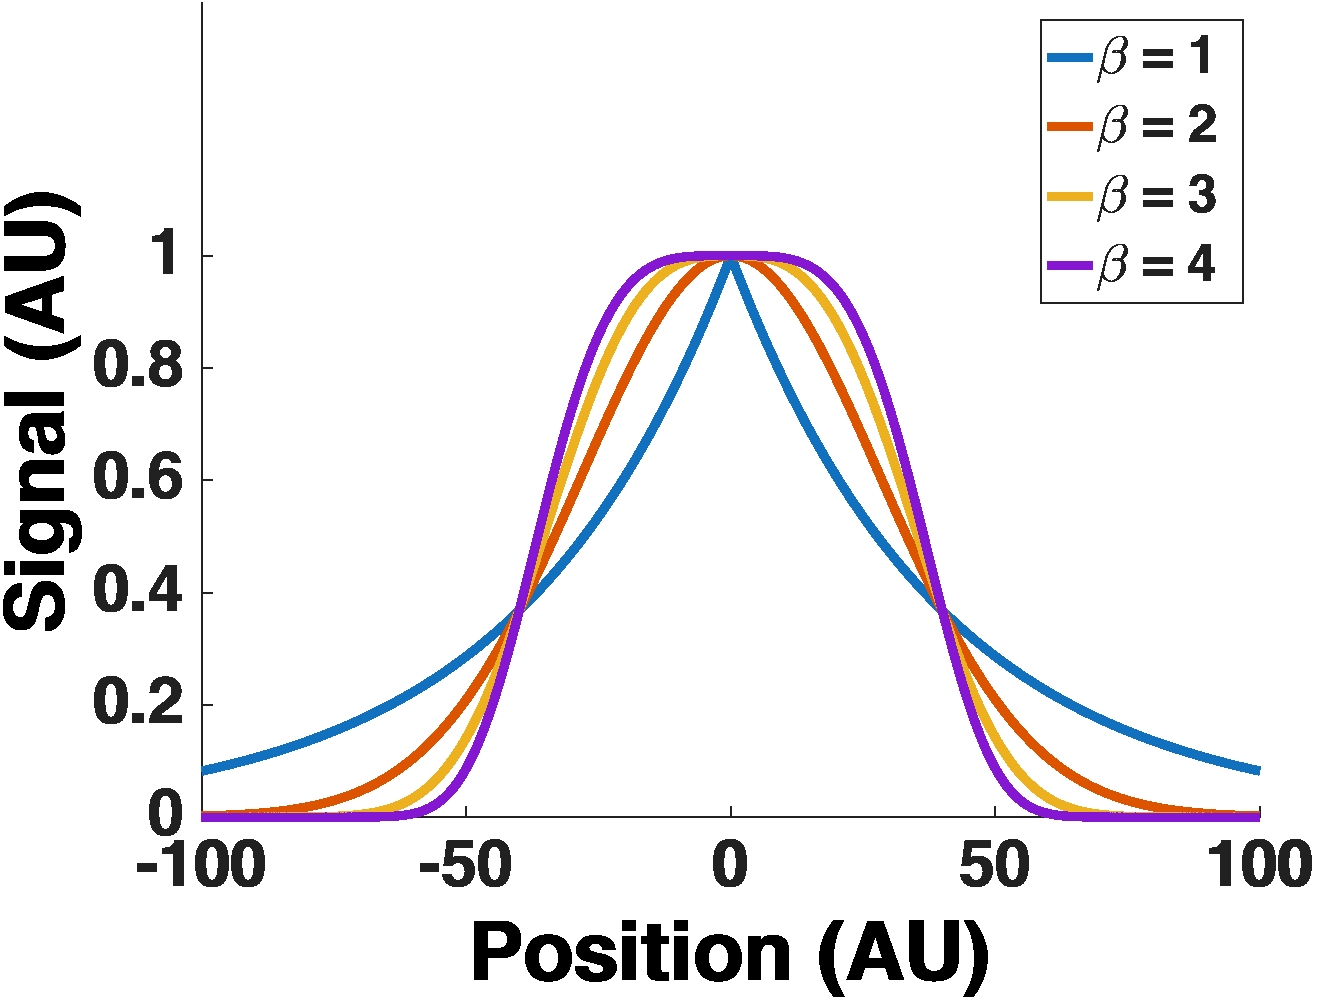
\includegraphics[height=3.8cm,keepaspectratio]{figures/gg_model_a.pdf}\end{subfigure}\hspace{0.02\linewidth}%
\begin{subfigure}[t]{0.38\linewidth}\centering\captionsetup{margin={6.25mm,0mm}}\caption{Model fits to MIP}\label{fig:gg_model_b}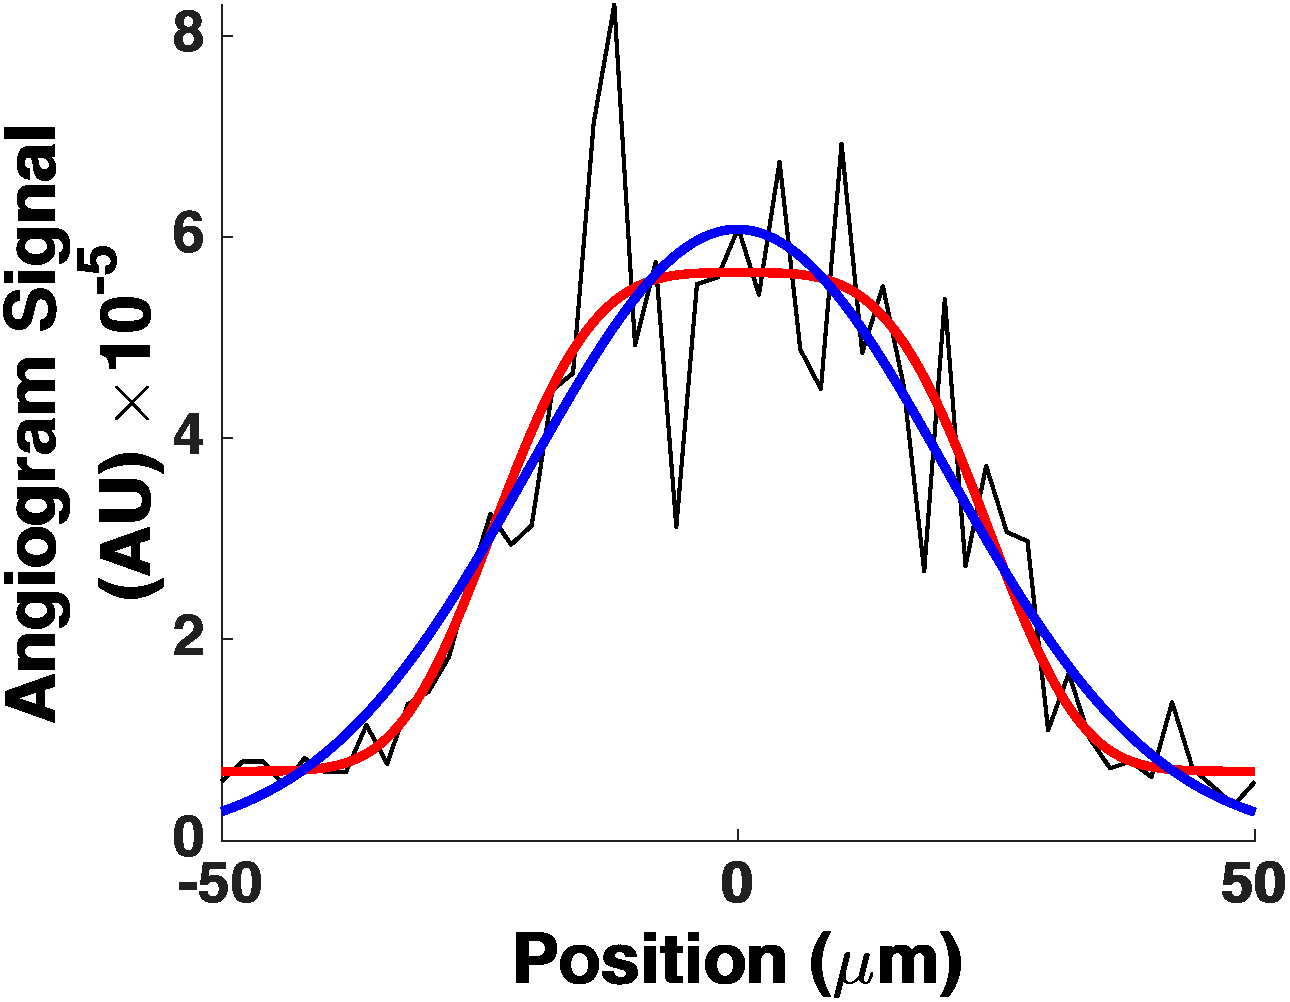
\includegraphics[height=3.8cm,keepaspectratio]{figures/gg_model_c.pdf}\end{subfigure}
\caption{(a) GG function for shape parameters $\beta = 1$, 2, 3, and 4.~(b) Example vessel intensity profile (black) taken from a MIP, with standard Gaussian (blue) and GG (red) fits. The MIP profile is flat-topped ($\beta = 3.7$), a shape the standard Gaussian cannot represent.}
\label{fig:gg_model}
\end{figure}

Two standard width metrics were calculated from the fitted models: the full width at half maximum (FWHM) and the $1/e^2$ width. For the standard Gaussian fit, the $1/e^2$ width was calculated as:
\begin{equation}
\label{eq:gauss_1e2}
w_{1/e^2,\,\mathrm{G}} = 4\sigma
\end{equation}
The FWHM for a Gaussian is related to the $1/e^2$ width by a fixed proportionality:
\begin{equation}
\label{eq:gauss_fwhm}
w_{fwhm,\,\mathrm{G}} = 2\sigma\sqrt{2\ln 2} = \frac{\sqrt{2\ln 2}}{2} \; w_{1/e^2,\,\mathrm{G}}
\end{equation}
and therefore only the $1/e^2$ width was calculated directly from the fit and evaluated here, with the FWHM obtainable via this known relationship.

For the GG fit, no such linear relationship exists between the FWHM and $1/e^2$ width, since both depend on the shape parameter $\beta$. Both metrics were therefore calculated independently as:
\begin{equation}
\label{eq:gg_fwhm}
w_{fwhm,\,\mathrm{GG}} = 2\alpha{\left(\ln 2\right)}^{1/\beta}
\end{equation}
\begin{equation}
\label{eq:gg_1e2}
w_{1/e^2,\,\mathrm{GG}} = 2\alpha \cdot 2^{1/\beta}
\end{equation}

\subsubsection{Binary-mask-based vessel diameter calculation}
\label{subsubsec:binary_mask}
For comparison with OCTA processing pipelines that rely on image binarisation, vessel diameters were also measured from binary masks generated by global thresholding. To determine the threshold level, the maximum angiogram intensity was measured after applying a 3D averaging filter with a kernel size of 50~$\times$~50~$\times$~10 voxels (lateral~$x$~$\times$~axial~$z$~$\times$~temporal~$t$) to the DyC-OCT angiogram volumes to reduce noise and minimise the effects of outliers. To produce a binary mask (BM), the maximum angiogram intensity within these smoothed volumes was calculated, and five different threshold values were defined as fixed percentages of these maxima for MIP and MeIP. For MIP, the thresholds were defined as BM-1~=~40\%, BM-2~=~50\%, BM-3~=~60\%, BM-4~=~70\%, and BM-5~=~80\%. While for MeIP, the thresholds were defined as BM-1~=~7\%, BM-2~=~8\%, BM-3~=~9\%, BM-4~=~10\%, and BM-5~=~11\%. These thresholds were selected empirically to cover the usable range of values for each projection. The upper and lower bounds were selected based on the point at which vessels began to be lost, and at which background noise and tissue signal were increasingly included, respectively. Each threshold was applied to the unsmoothed en face projection (MIP and MeIP) to generate a binary mask, and the vessel diameter was measured as the number of pixels above the threshold across the lateral vessel cross-section.

\subsubsection{Statistical analysis}
\label{subsubsec:stats}
To evaluate the accuracy and precision of all diameter measurement approaches, the calculated diameter values were plotted against the ground truth for each vessel across three conditions: pre-contrast, peak contrast, and post-contrast. A linear regression was fitted to each condition, yielding the slope ($m$) and coefficient of determination ($R^2$). A slope of $m = 1$ indicated perfect agreement with the ground truth, and $R^2$ quantified the goodness of fit of the linear model, indicating how well it can be corrected by a calibrated scaling factor. Additionally, the coefficient of variation (CoV) was computed for each vessel across the time samples within each contrast condition and then averaged across vessels, to assess measurement precision (repeatability). For the model-based methods, six combinations were evaluated: two projection methods (MIP and MeIP) by three width metrics ($w_{1/e^2,\,\mathrm{G}}$, $w_{fwhm,\,\mathrm{GG}}$, and $w_{1/e^2,\,\mathrm{GG}}$). For the binary-mask-based method, diameter was measured at five threshold levels (BM-1 through BM-5) for both MIP and MeIP. For the functional flicker stimulation experiment, a paired t-test was used to evaluate whether vessel diameters differed significantly between the pre- and post-stimulation windows, and the Pearson correlation coefficient ($\rho$) between measured diameter values and angiogram intensity was computed for each method and vessel to assess whether the diameter measurements were affected by changes in angiogram intensity. Measurements with $p < 0.05$ were considered statistically significant (significance levels: $^{*}p < 0.05$, $^{**}p < 0.01$, $^{***}p < 0.001$). 

\section{Results}
\subsection{Qualitative assessment of vessel underestimation}
\label{subsec:qualitative}

\begin{figure}[p]
\centering
\setlength{\abovecaptionskip}{4pt}\setlength{\belowcaptionskip}{2pt}
\setlength{\tabcolsep}{0pt}
\renewcommand{\arraystretch}{0}
\begin{tabular}{@{}c@{\hspace{3pt}}c@{\hspace{2pt}}c@{}}
 & \textbf{Pre-Contrast} & \textbf{Post-Contrast} \\[3pt]
\raisebox{-0.5\height}{\rotatebox{90}{\textbf{SVP}}} &
  \raisebox{-0.5\height}{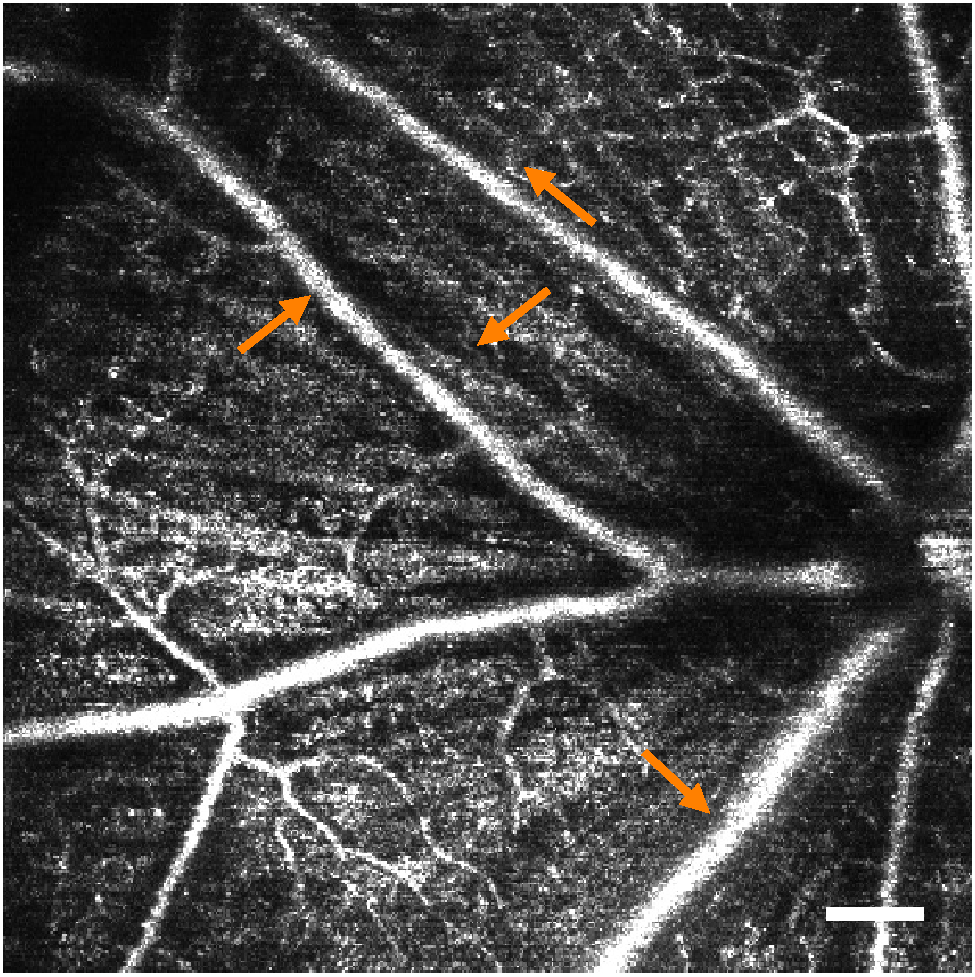
\includegraphics[width=2.8cm]{figures/enface_svp_pre.pdf}} &
  \raisebox{-0.5\height}{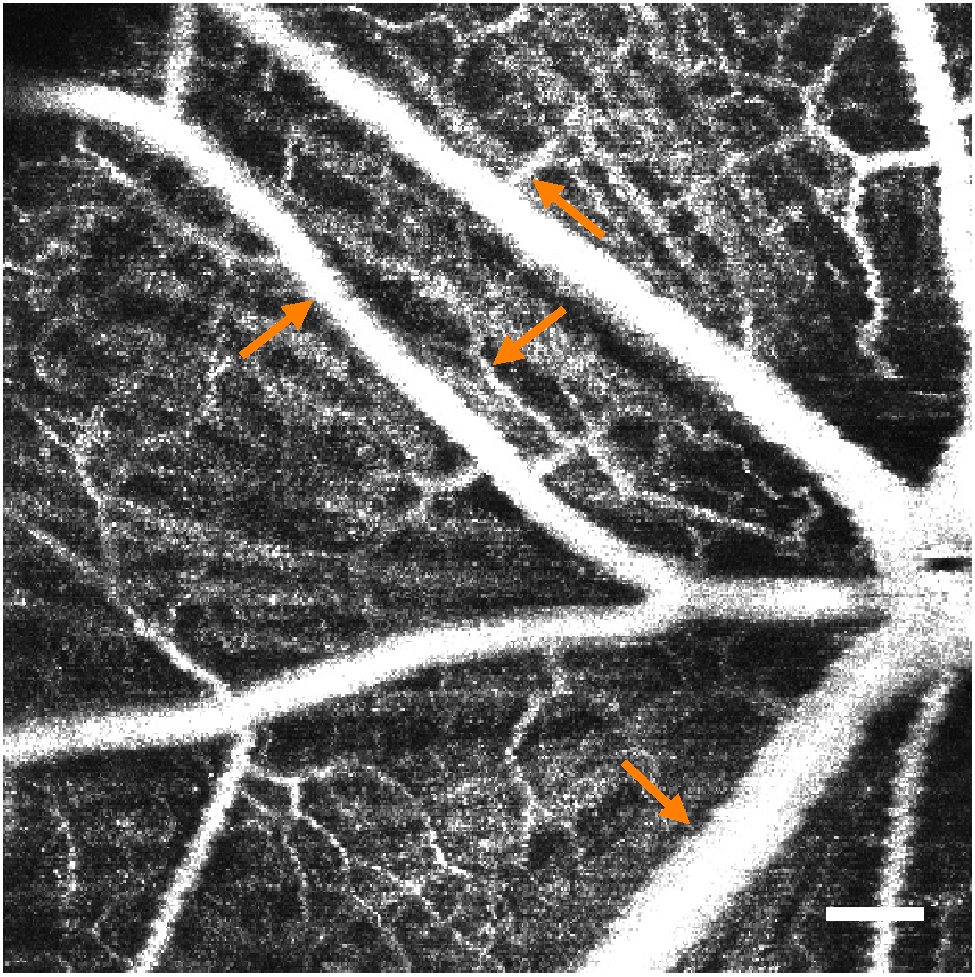
\includegraphics[width=2.8cm]{figures/enface_svp_post.pdf}} \\[2pt]
\raisebox{-0.5\height}{\rotatebox{90}{\textbf{ICP}}} &
  \raisebox{-0.5\height}{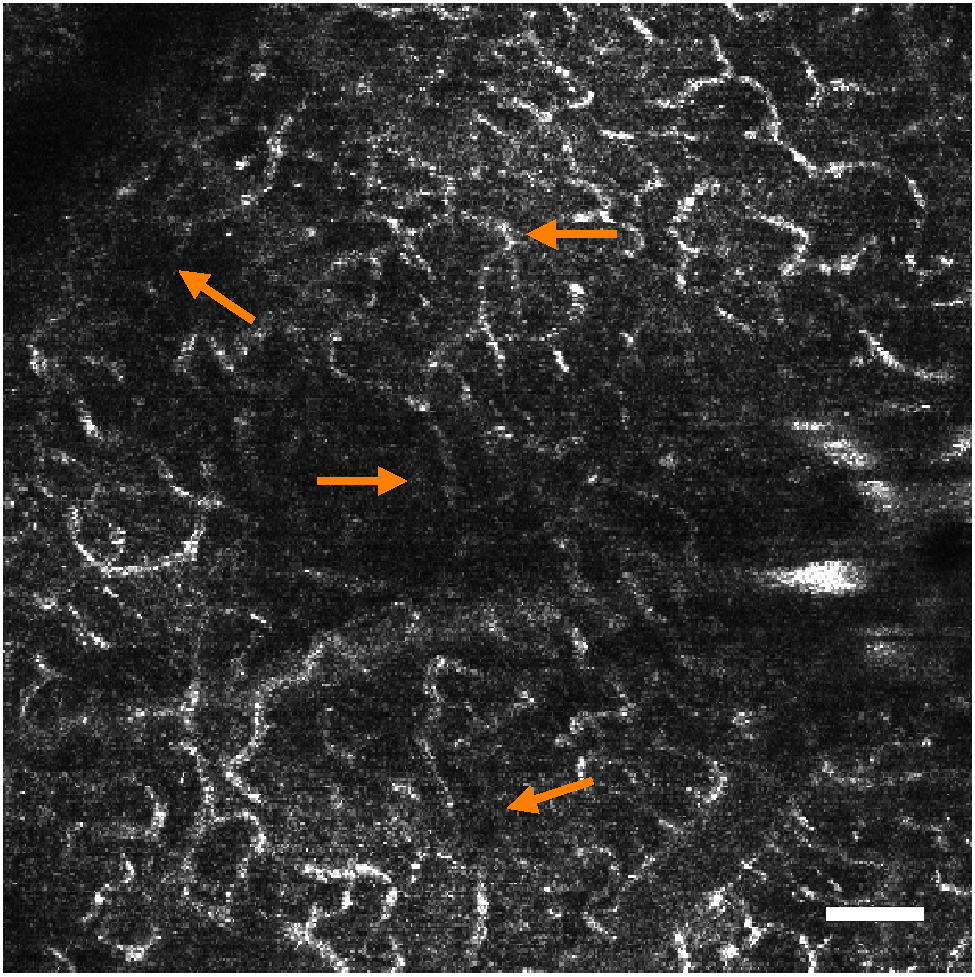
\includegraphics[width=2.8cm]{figures/enface_icp_pre.pdf}} &
  \raisebox{-0.5\height}{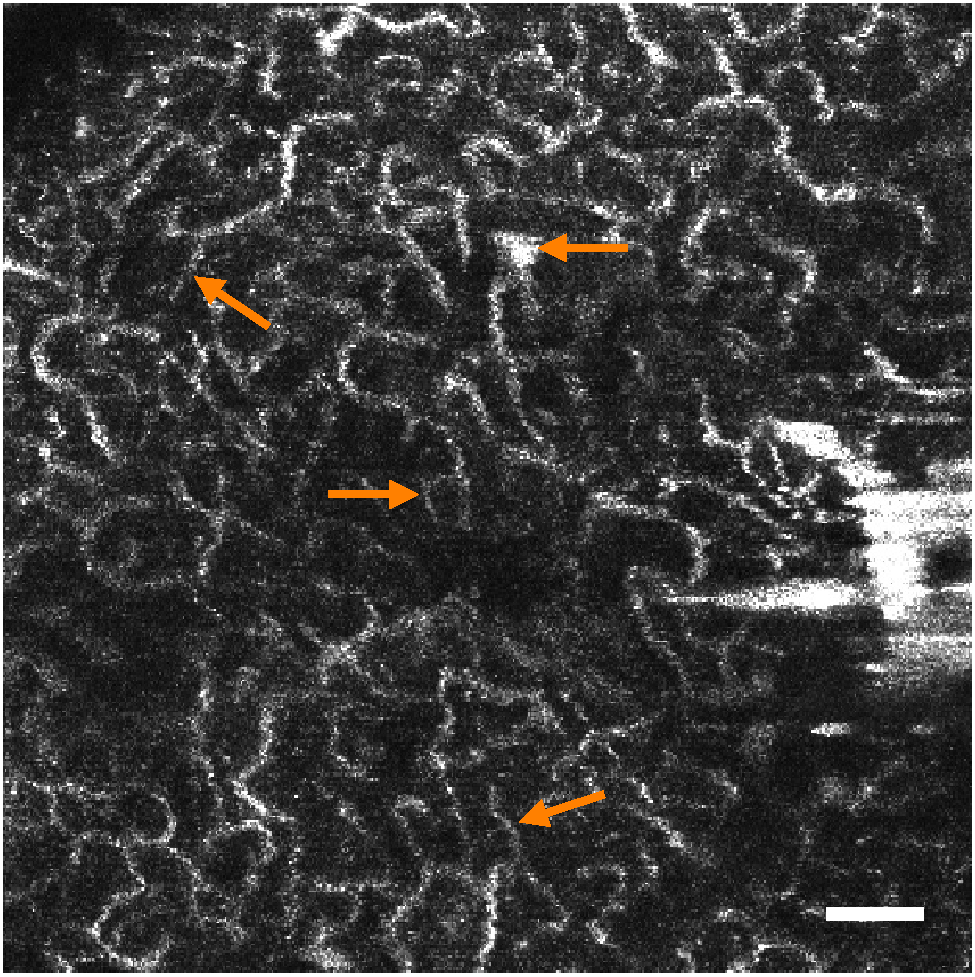
\includegraphics[width=2.8cm]{figures/enface_icp_post.pdf}} \\[2pt]
\raisebox{-0.5\height}{\rotatebox{90}{\textbf{DCP}}} &
  \raisebox{-0.5\height}{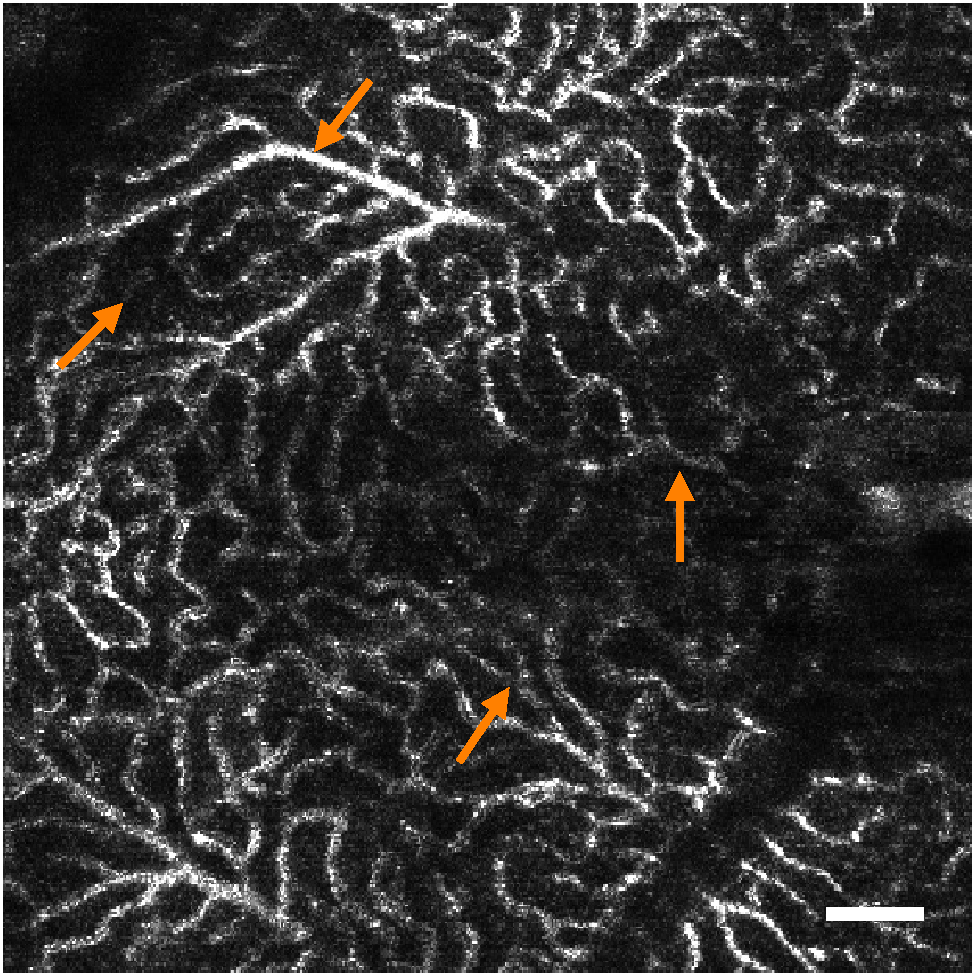
\includegraphics[width=2.8cm]{figures/enface_dcp_pre.pdf}} &
  \raisebox{-0.5\height}{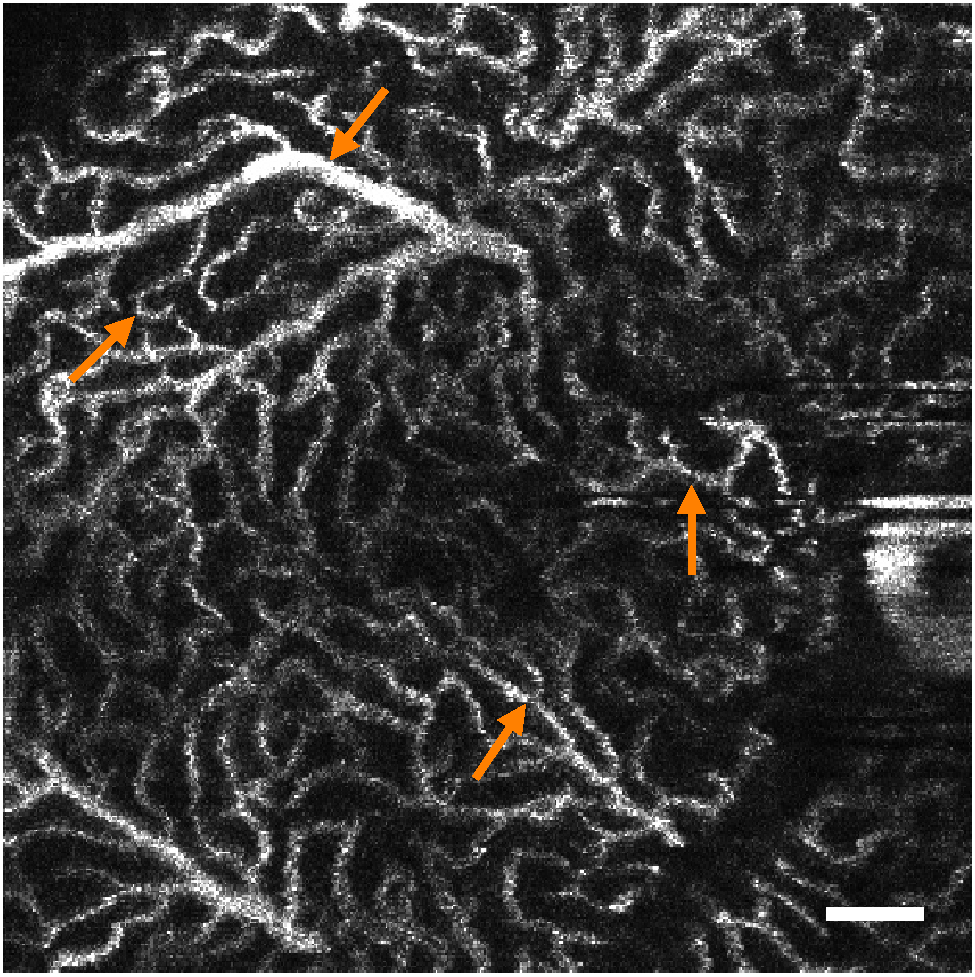
\includegraphics[width=2.8cm]{figures/enface_dcp_post.pdf}} \\
\end{tabular}
\caption{En face OCTA maximum intensity projections of the SVP, ICP, and DCP before (left) and after (right) the administration of Intralipid 20\%. Vessels appear visibly wider and brighter post-contrast across all layers, most prominently in the larger vessels. Orange arrows point to vessels that show an apparent change in diameter or that were barely visible pre-contrast. All scale bars are 100\,\textmu{}m. Display ranges were set within each pair to give an equal background noise level.}
\label{fig:enface_contrast}
\end{figure}

\begin{figure}[p]
\centering
\setlength{\abovecaptionskip}{4pt}\setlength{\belowcaptionskip}{2pt}
\captionsetup[subfigure]{position=top,font=bf,skip=1pt}
\begin{minipage}[t]{0.38\linewidth}\vspace{6pt}
{\centering\small\bfseries B-scan angiogram\par}\vspace{1pt}
\offinterlineskip
\begin{subfigure}[t]{\linewidth}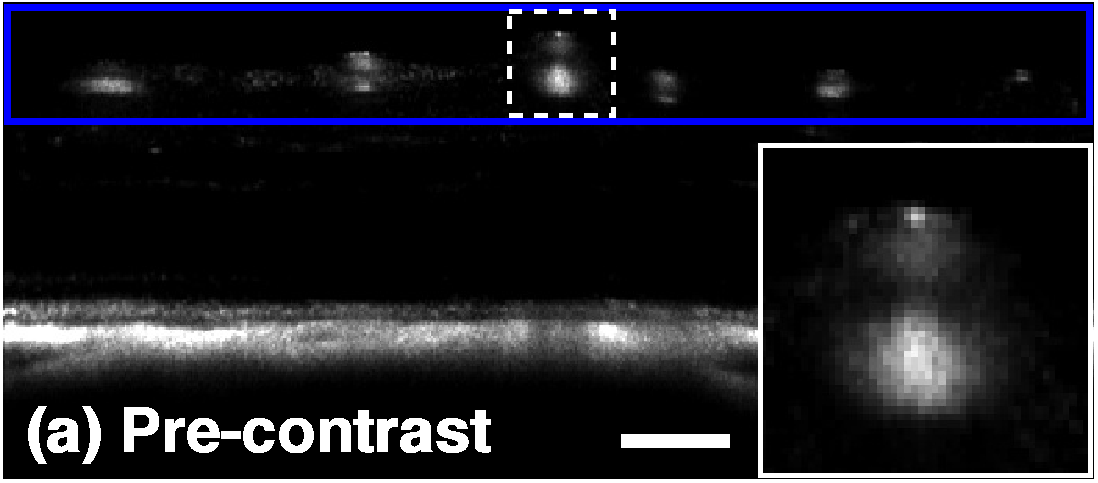
\includegraphics[width=\linewidth]{figures/dycoct_a.pdf}\phantomsubcaption\label{fig:dycoct_a}\end{subfigure}\\
\begin{subfigure}[t]{\linewidth}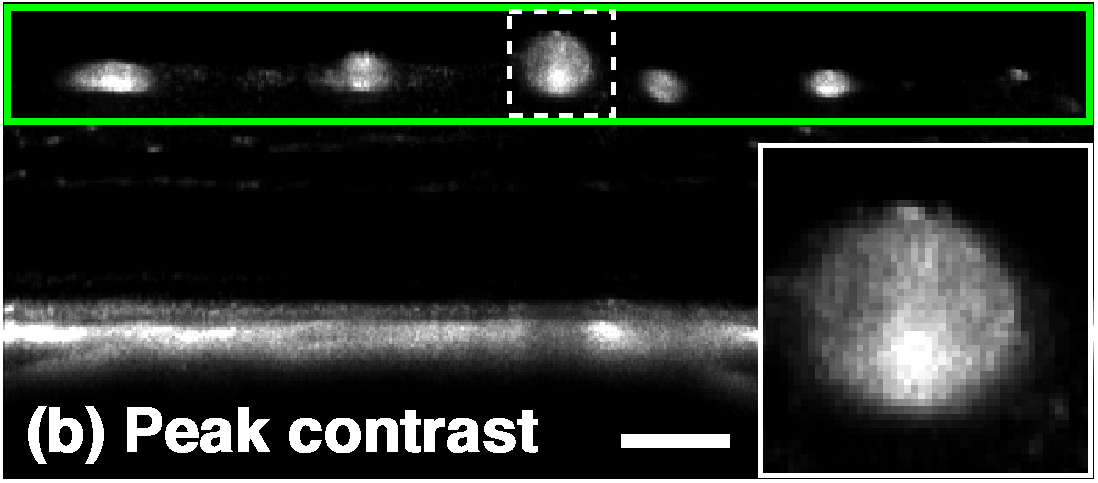
\includegraphics[width=\linewidth]{figures/dycoct_b.pdf}\phantomsubcaption\label{fig:dycoct_b}\end{subfigure}\\
\begin{subfigure}[t]{\linewidth}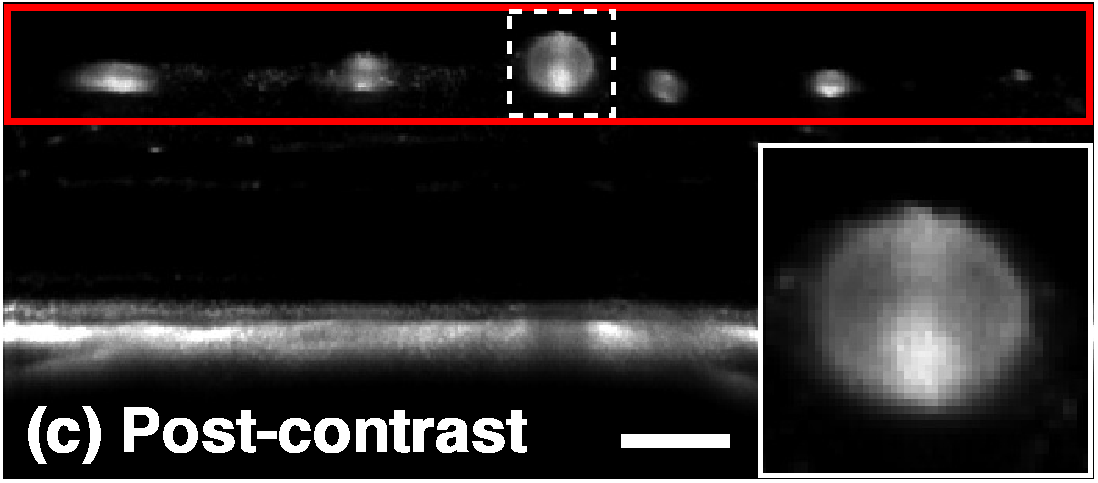
\includegraphics[width=\linewidth]{figures/dycoct_c.pdf}\phantomsubcaption\label{fig:dycoct_c}\end{subfigure}
\end{minipage}\hfill%
\begin{minipage}[t]{0.60\linewidth}\vspace{0pt}
\begin{subfigure}[t]{0.49\linewidth}\centering\captionsetup{margin={5.5mm,0mm}}\caption{MIP over time}\label{fig:dycoct_d}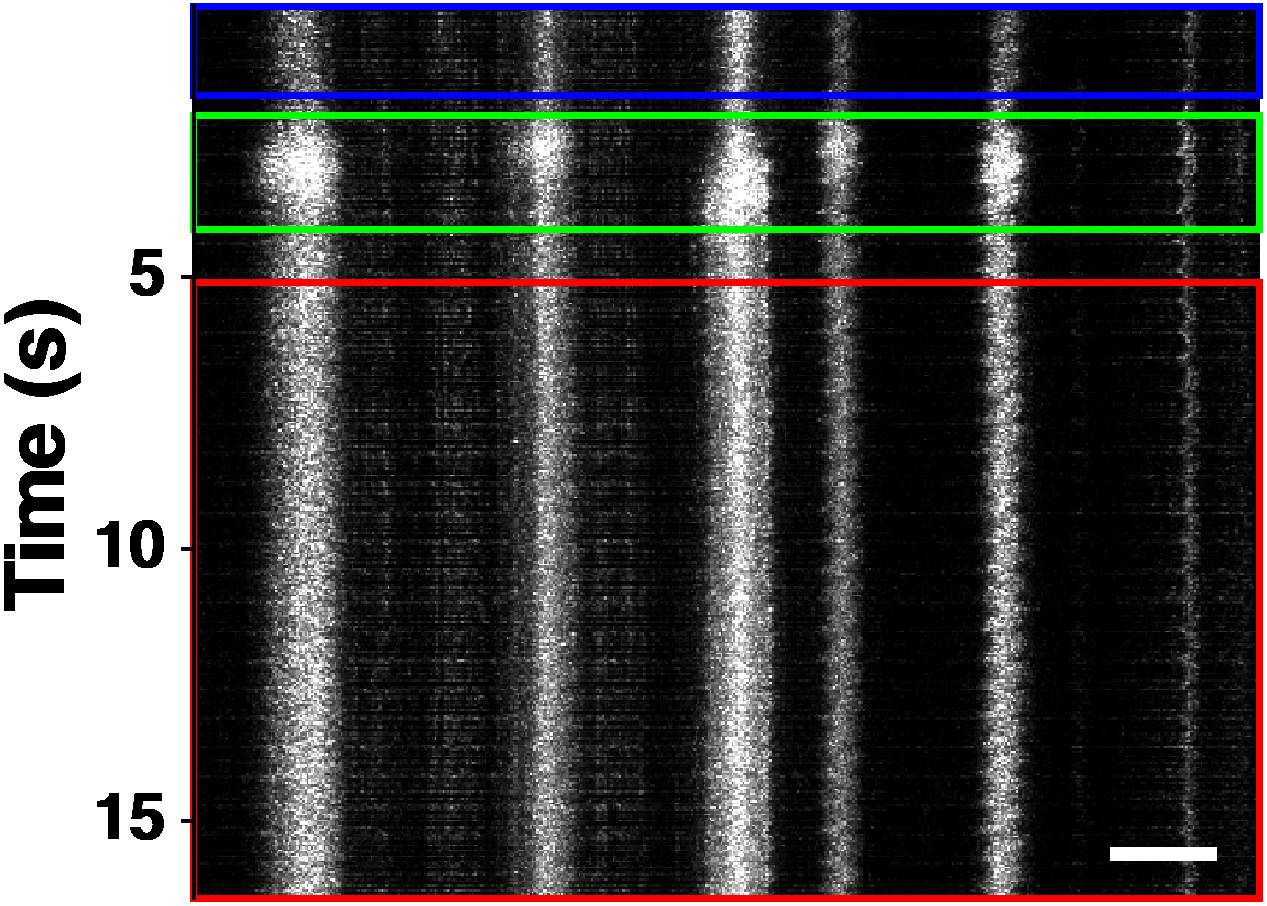
\includegraphics[height=2.75cm,keepaspectratio]{figures/dycoct_d.pdf}\end{subfigure}\hfill%
\begin{subfigure}[t]{0.49\linewidth}\centering\captionsetup{margin={5.5mm,0mm}}\caption{Binarised MIP}\label{fig:dycoct_e}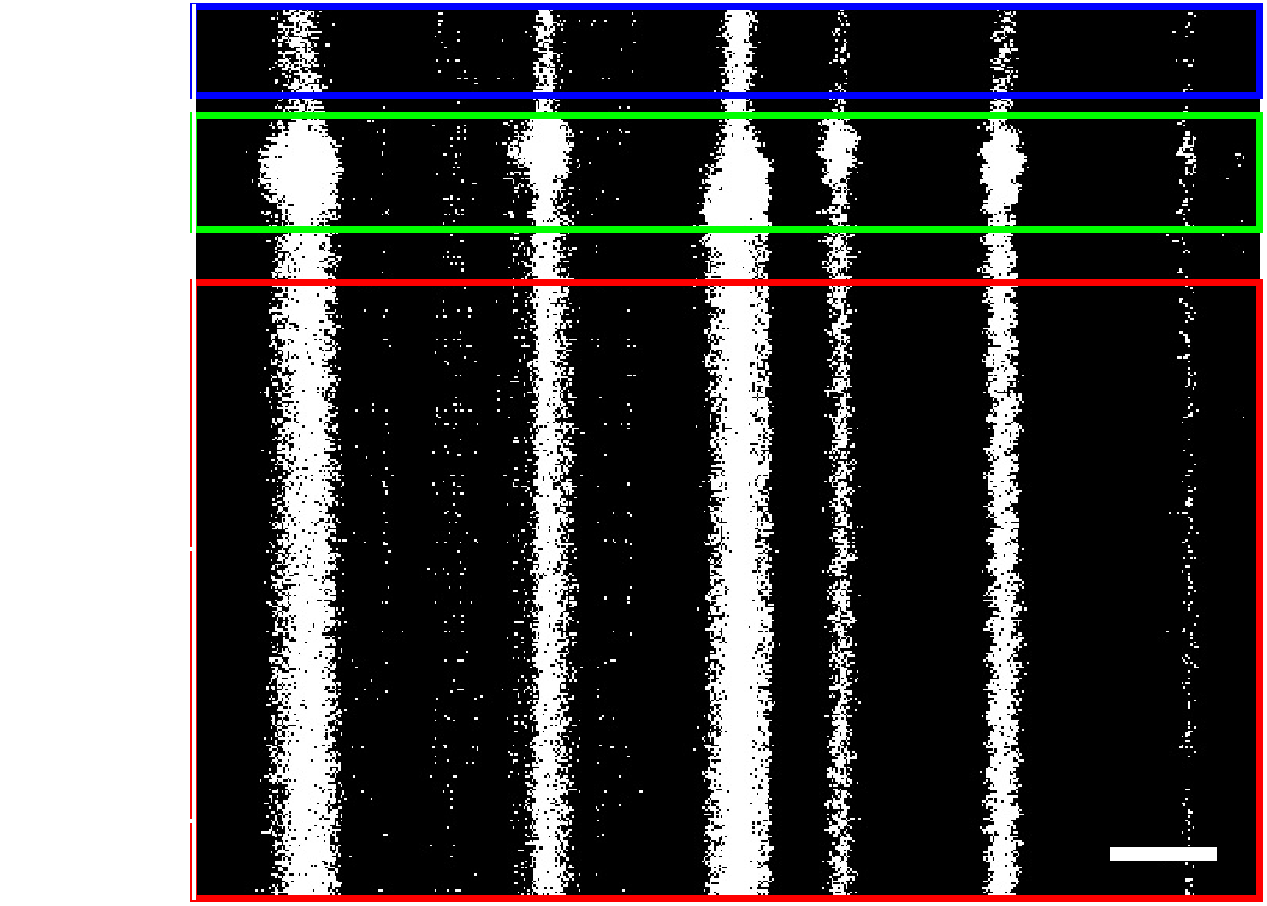
\includegraphics[height=2.75cm,keepaspectratio]{figures/dycoct_e.pdf}\end{subfigure}\\[6pt]
\begin{subfigure}[t]{\linewidth}\centering\captionsetup{margin={4.5mm,0mm}}\caption{Mean intensity}\label{fig:dycoct_f}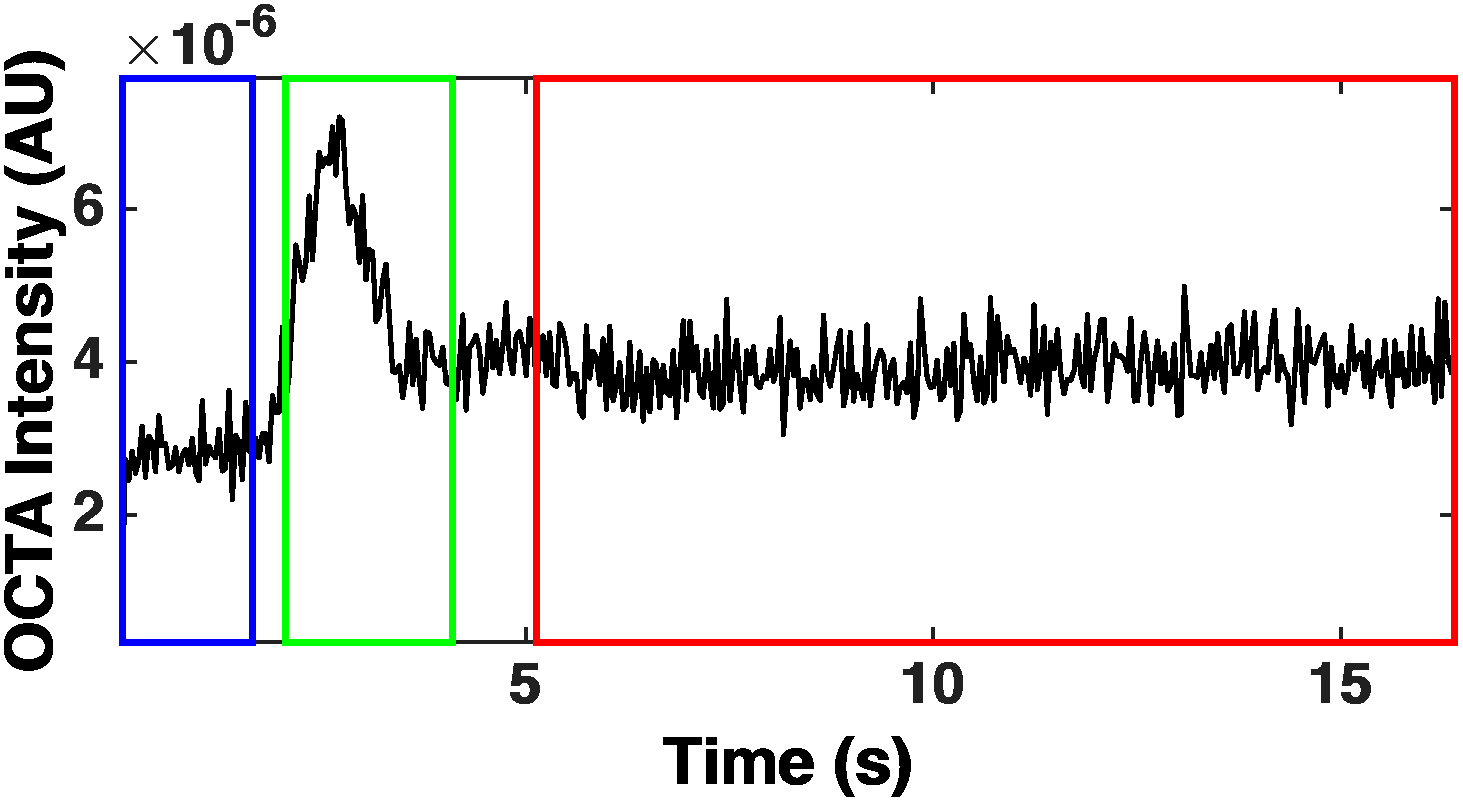
\includegraphics[height=3.17cm,keepaspectratio]{figures/dycoct_f.pdf}\end{subfigure}
\end{minipage}
\caption{DyC-OCT B-scan angiograms at (a) pre-contrast, (b) peak contrast, and (c) post-contrast, with insets showing a zoomed view of a single vessel cross-section.~(d) MIP and (e) binarisation of the vessel cross-sections over time. Coloured boxes indicate pre-contrast (blue), peak-contrast (green), and post-contrast (red) windows.~(f) Mean OCTA intensity over time. All scale bars are 100\,\textmu{}m.}
\label{fig:dycoct}
\end{figure}

Figure~\ref{fig:enface_contrast} shows en face OCTA maximum intensity projections of the superficial vascular plexus (SVP), intermediate capillary plexus (ICP), and deep capillary plexus (DCP) before and after contrast injection. Across all three layers, vessels appeared visibly wider and brighter post-contrast injection, consistent with previous literature~\cite{merkleHighresolutionDepthresolvedVascular2021}. This effect was most pronounced in the larger vessels, especially in the SVP, where the major retinal arteries and veins appeared noticeably thicker after contrast administration. In the ICP and DCP, the capillary networks also showed improved visibility, though the effect was less dramatic.

DyC OCTA projections helped visualise the temporal changes in vessel diameter pre- and post-contrast injection (Fig.~\ref{fig:dycoct}). Pre-contrast injection, the vessel cross-sections appeared narrower than in the contrast-enhanced phase (Fig.~\ref{fig:dycoct}a), which is due to lateral edge signal suppression by the RBC orientation artefact~\cite{bernucciInvestigationArtifactsRetinal2018}. At peak contrast, the Intralipid filled the vascular lumen completely. The vessels appeared slightly wider at peak than post-contrast, but this could be due to the dynamic range of the image rather than a true diameter change (Fig.~\ref{fig:dycoct}b). In the post-contrast phase, the signal stabilised as the initial bolus cleared, and the vessel boundaries remained more visible than before injection (Fig.~\ref{fig:dycoct}c). The MIP and the corresponding binary mask over time (Figs.~\ref{fig:dycoct}d,e) showed the observed temporal changes in vessel diameter across the three phases. The mean OCTA intensity (Fig.~\ref{fig:dycoct}f) showed a sharp increase post-contrast injection, followed by a decrease to a new steady state that remained elevated above the pre-contrast baseline. 

\subsection{Accuracy and precision of diameter measurements}
\label{subsec:accuracy_precision}
All methods underestimated vessel diameter in pre-contrast data, with slopes ranging from 0.42 to 0.73 (Table~\ref{tab:accuracy_linearity}). Contrast enhancement improved accuracy across all metrics, though the degree of improvement varied. 

\begin{figure}[p]
\centering
\setlength{\abovecaptionskip}{4pt}\setlength{\belowcaptionskip}{2pt}
\captionsetup[subfigure]{position=top,font=bf,skip=2pt}
\begin{subfigure}{0.27\linewidth}\centering\captionsetup{margin={3.60mm,0mm}}\caption{MIP $w_{1/e^2,\,\mathrm{G}}$}\label{fig:scatter_model_a}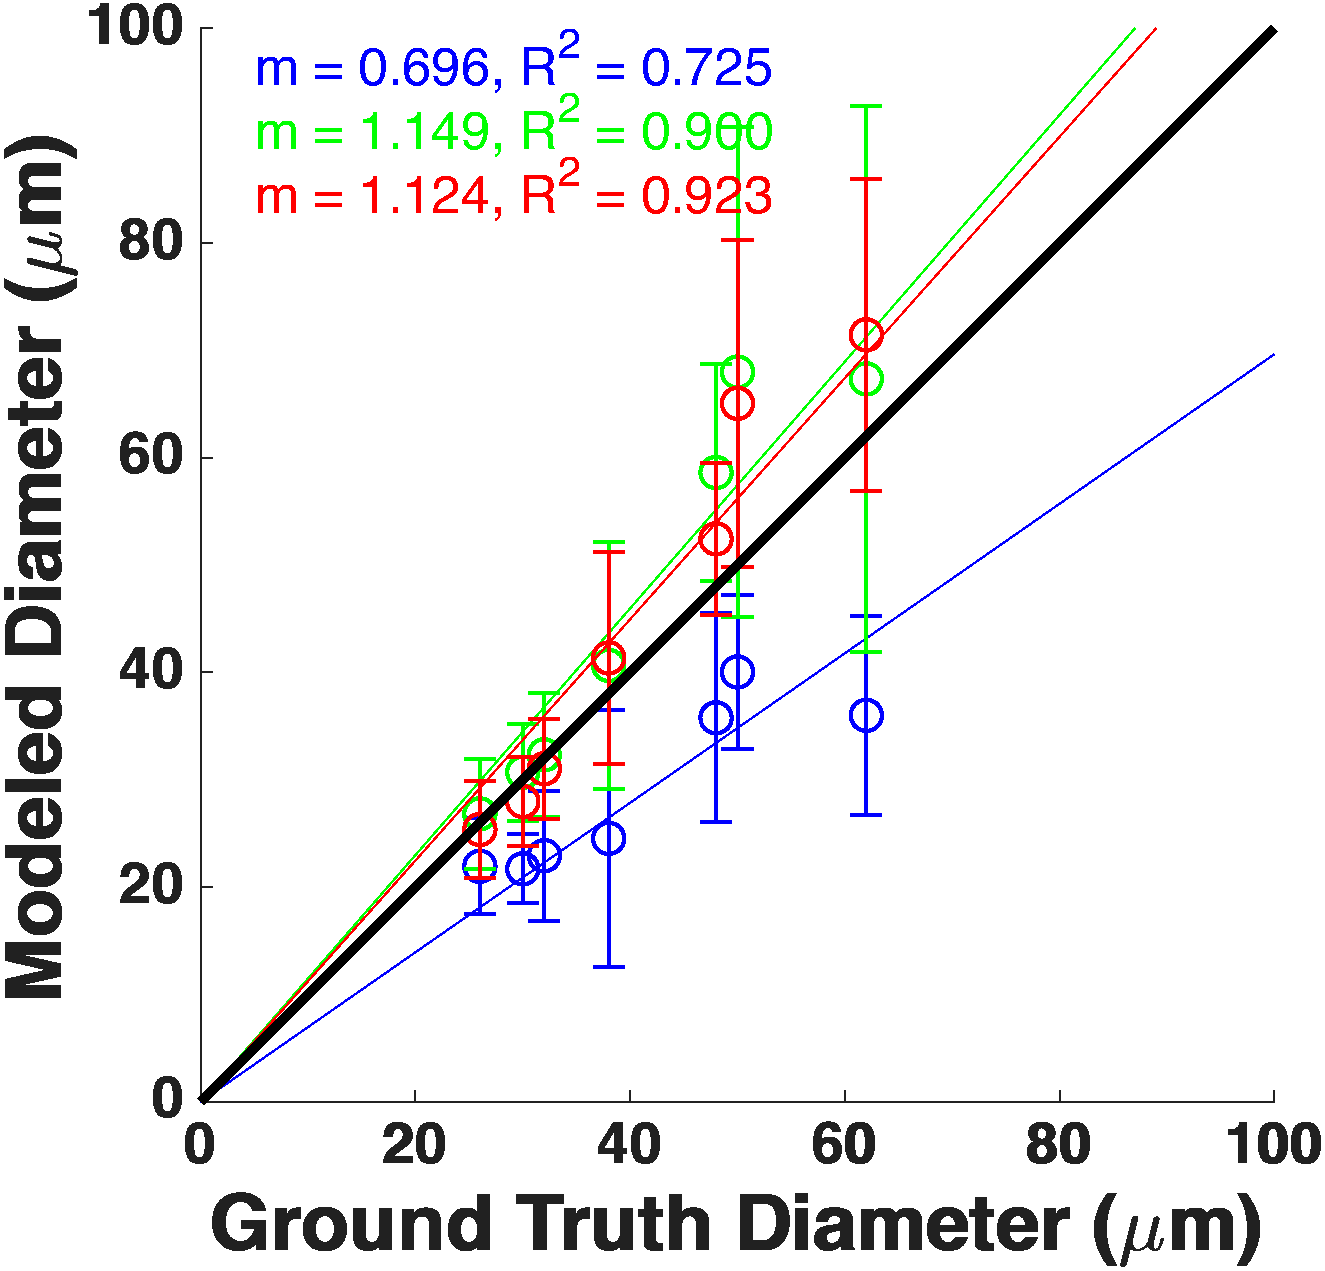
\includegraphics[width=\linewidth]{figures/scatter_model_a.pdf}\end{subfigure}\hfill%
\begin{subfigure}{0.27\linewidth}\centering\captionsetup{margin={3.60mm,0mm}}\caption{MIP $w_{fwhm,\,\mathrm{GG}}$}\label{fig:scatter_model_b}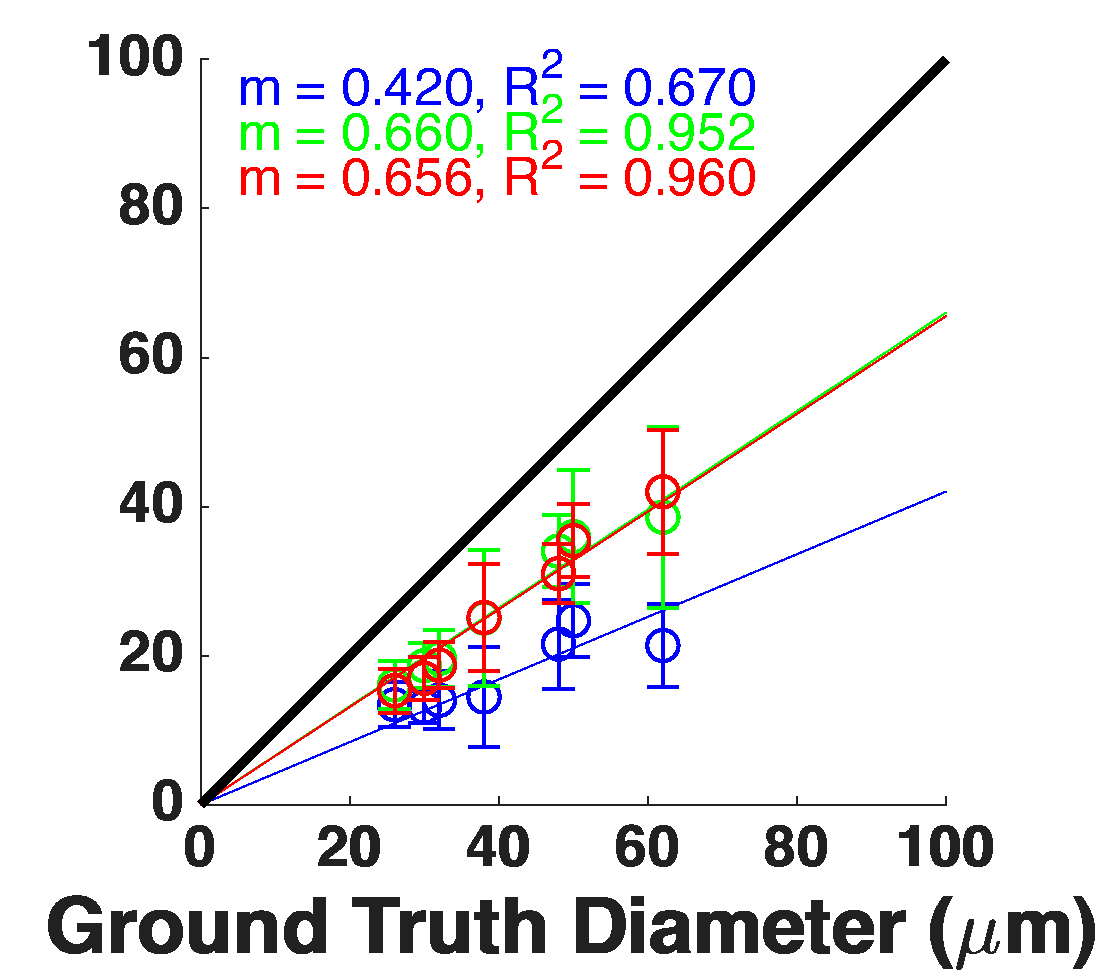
\includegraphics[width=\linewidth]{figures/scatter_model_b.pdf}\end{subfigure}\hfill%
\begin{subfigure}{0.27\linewidth}\centering\captionsetup{margin={3.60mm,0mm}}\caption{MIP $w_{1/e^2,\,\mathrm{GG}}$}\label{fig:scatter_model_c}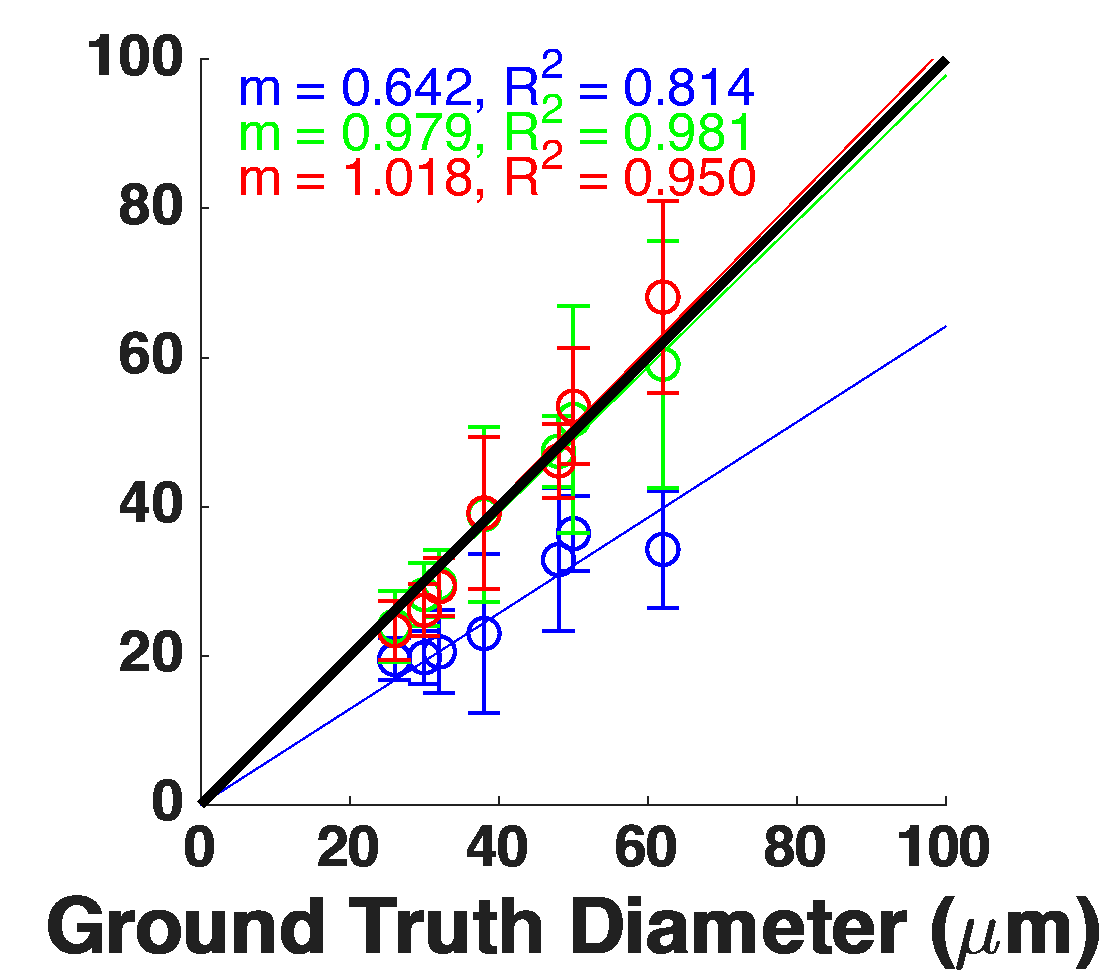
\includegraphics[width=\linewidth]{figures/scatter_model_c.pdf}\end{subfigure}\\[2pt]
\begin{subfigure}{0.27\linewidth}\centering\captionsetup{margin={3.60mm,0mm}}\caption{MeIP $w_{1/e^2,\,\mathrm{G}}$}\label{fig:scatter_model_d}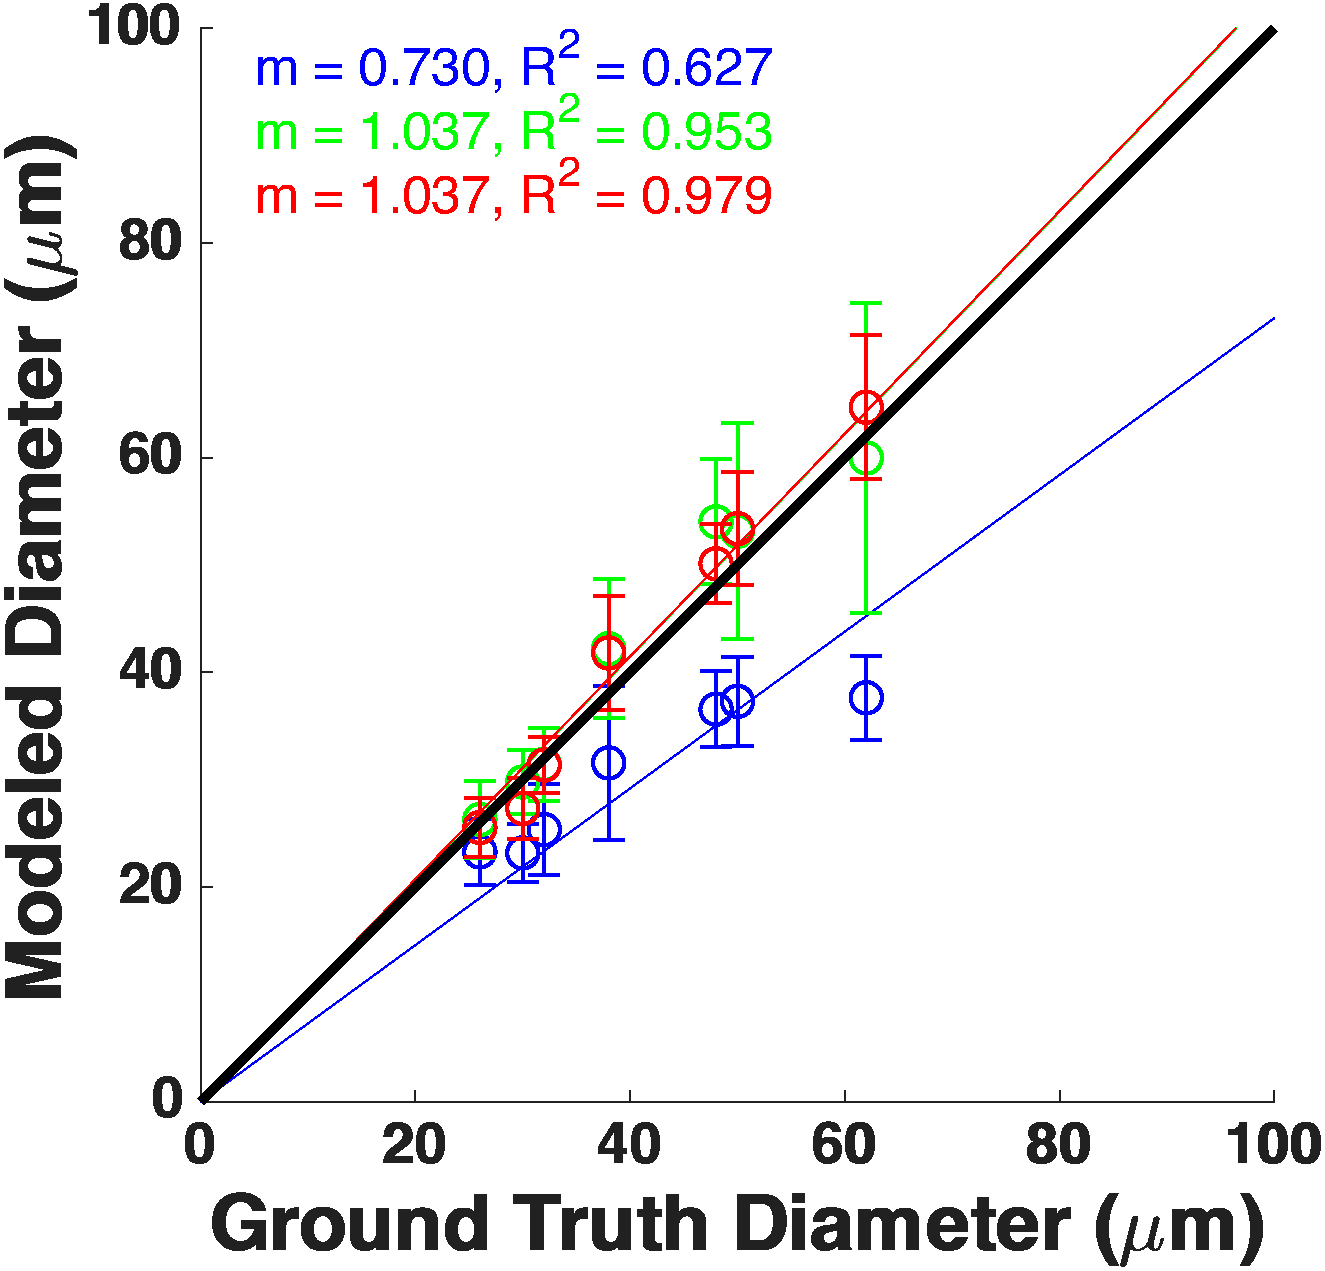
\includegraphics[width=\linewidth]{figures/scatter_model_d.pdf}\end{subfigure}\hfill%
\begin{subfigure}{0.27\linewidth}\centering\captionsetup{margin={3.60mm,0mm}}\caption{MeIP $w_{fwhm,\,\mathrm{GG}}$}\label{fig:scatter_model_e}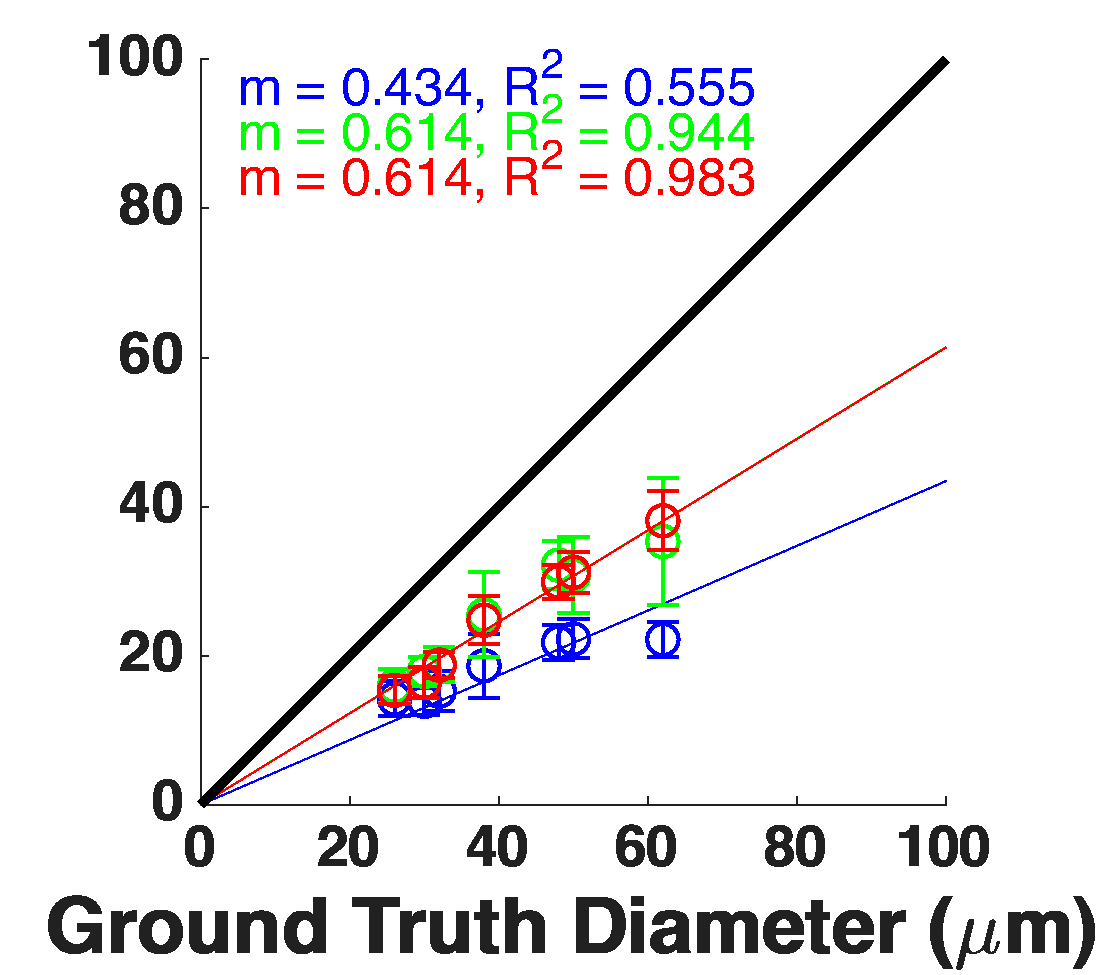
\includegraphics[width=\linewidth]{figures/scatter_model_e.pdf}\end{subfigure}\hfill%
\begin{subfigure}{0.27\linewidth}\centering\captionsetup{margin={3.60mm,0mm}}\caption{MeIP $w_{1/e^2,\,\mathrm{GG}}$}\label{fig:scatter_model_f}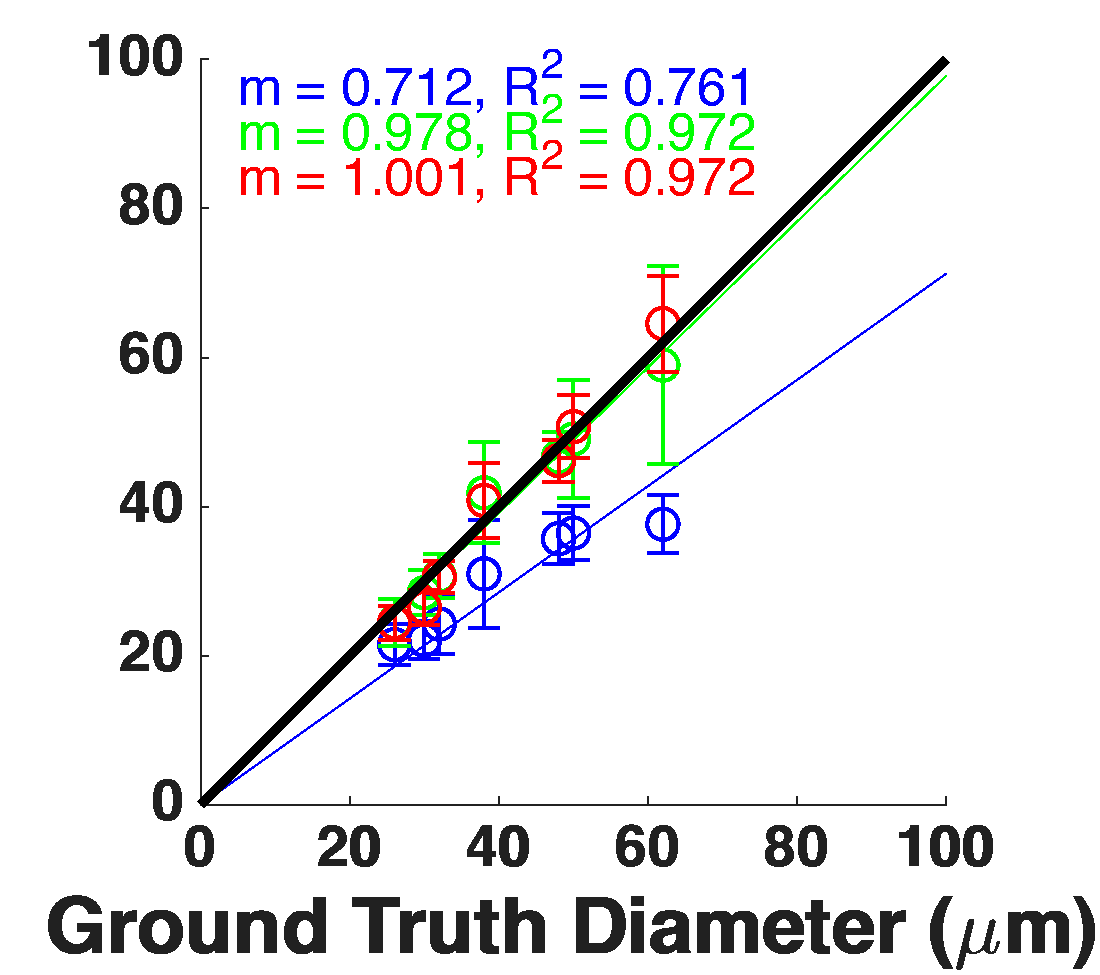
\includegraphics[width=\linewidth]{figures/scatter_model_f.pdf}\end{subfigure}
\caption{Modelled versus ground truth vessel diameter using MIP (top row, a--c) and MeIP (bottom row, d--f). Columns correspond to $w_{1/e^2,\,\mathrm{G}}$ (a, d), $w_{fwhm,\,\mathrm{GG}}$ (b, e), and $w_{1/e^2,\,\mathrm{GG}}$ (c, f). Linear regression lines and statistics are shown for pre-contrast (blue), peak contrast (green), and post-contrast (red) conditions. The black line indicates the identity line ($m = 1$).}
\label{fig:scatter_model}\par\vspace{2pt}
\end{figure}

\begin{figure}[p]
\centering
\setlength{\abovecaptionskip}{4pt}\setlength{\belowcaptionskip}{2pt}
\captionsetup[subfigure]{position=top,font=bf,skip=2pt}
\begin{subfigure}{0.27\linewidth}\centering\captionsetup{margin={3.60mm,0mm}}\caption{MIP, BM-1}\label{fig:scatter_bw_mip_a}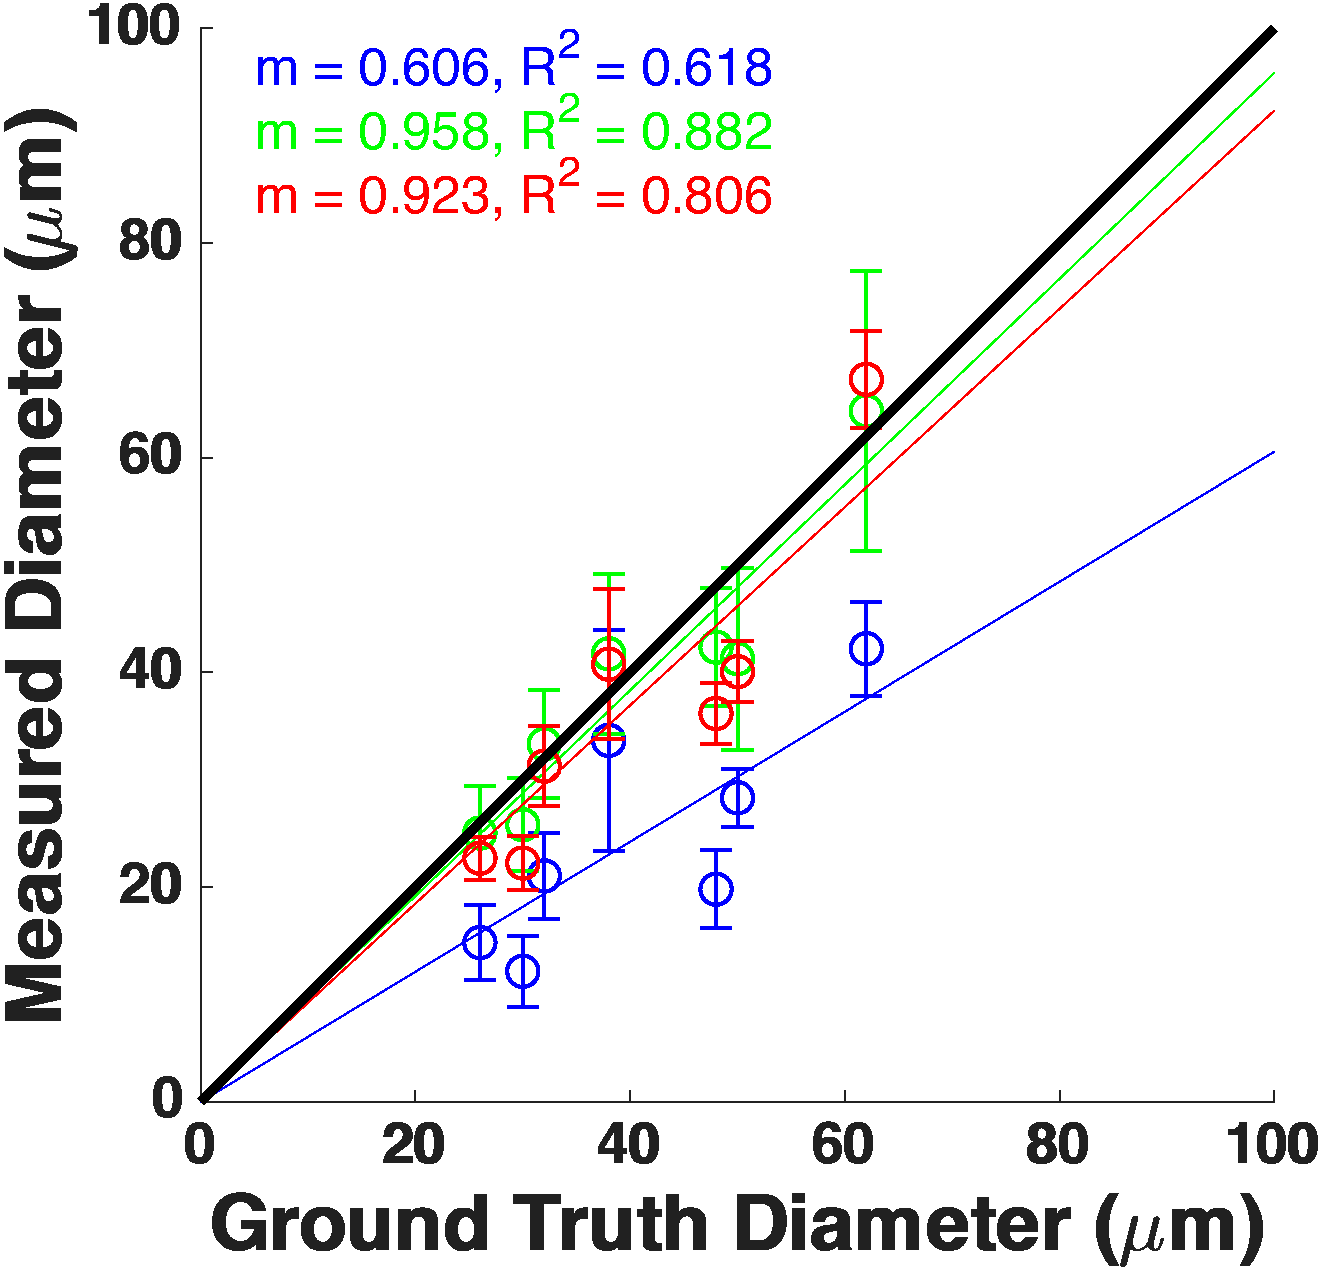
\includegraphics[width=\linewidth]{figures/scatter_bw_mip_a.pdf}\end{subfigure}\hfill%
\begin{subfigure}{0.27\linewidth}\centering\captionsetup{margin={3.60mm,0mm}}\caption{MIP, BM-2}\label{fig:scatter_bw_mip_b}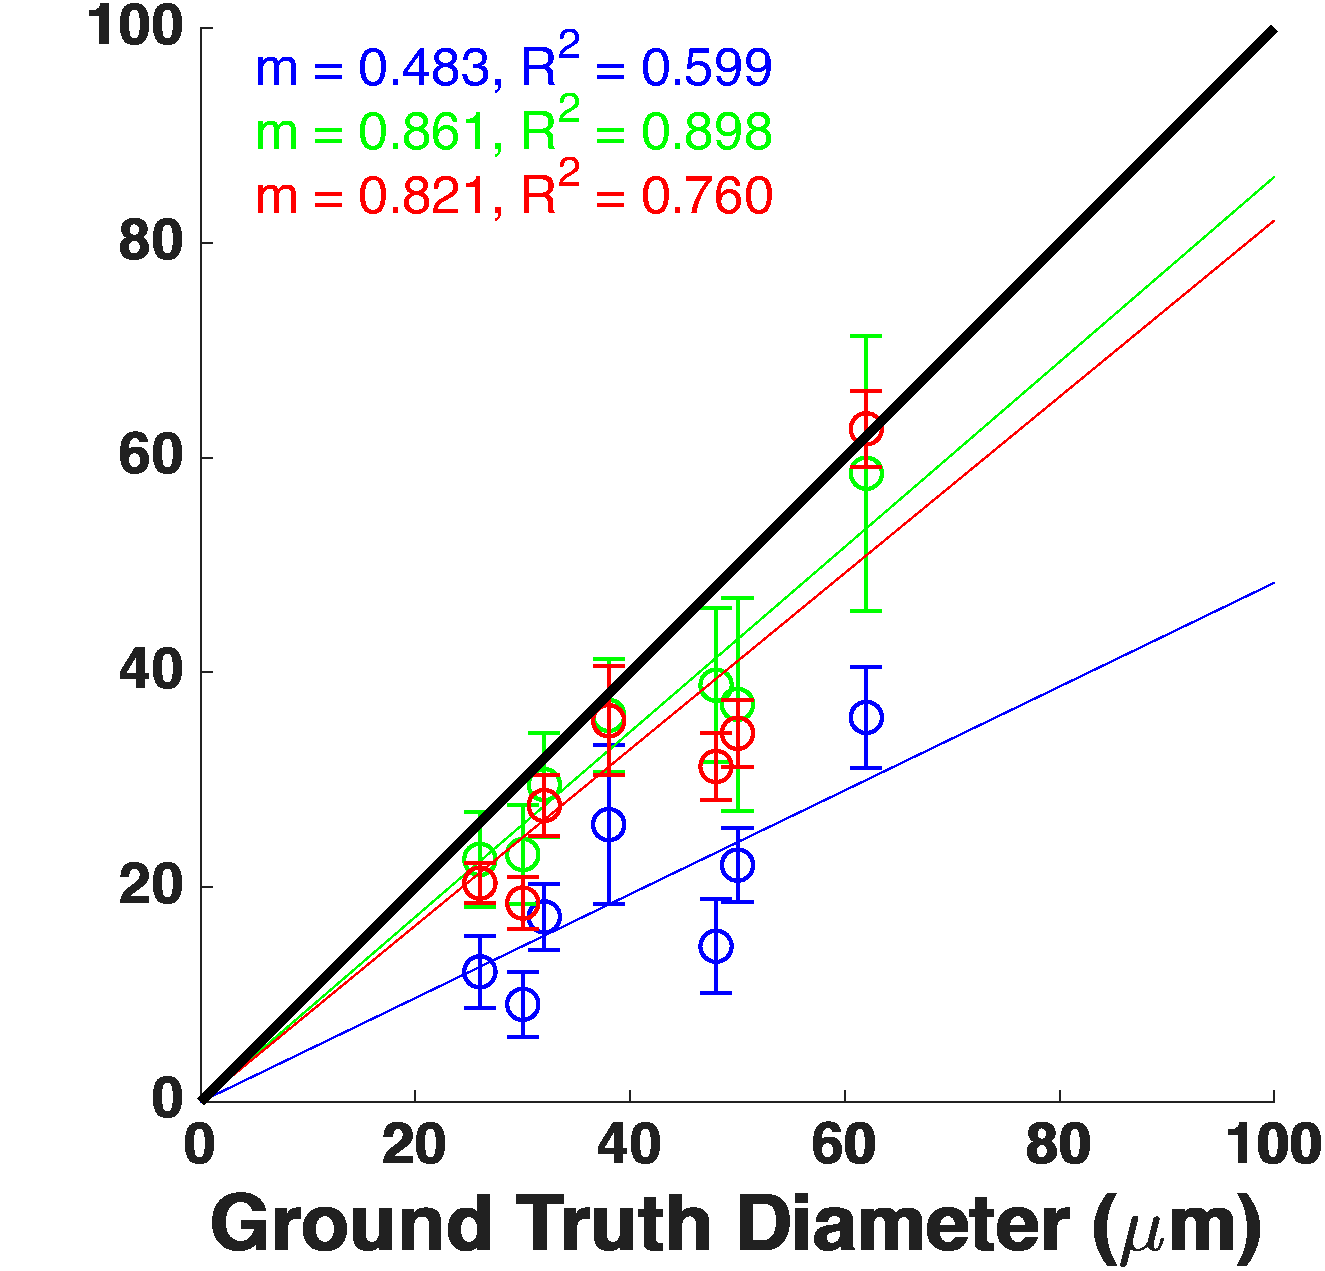
\includegraphics[width=\linewidth]{figures/scatter_bw_mip_b.pdf}\end{subfigure}\hfill%
\begin{subfigure}{0.27\linewidth}\centering\captionsetup{margin={3.60mm,0mm}}\caption{MIP, BM-3}\label{fig:scatter_bw_mip_c}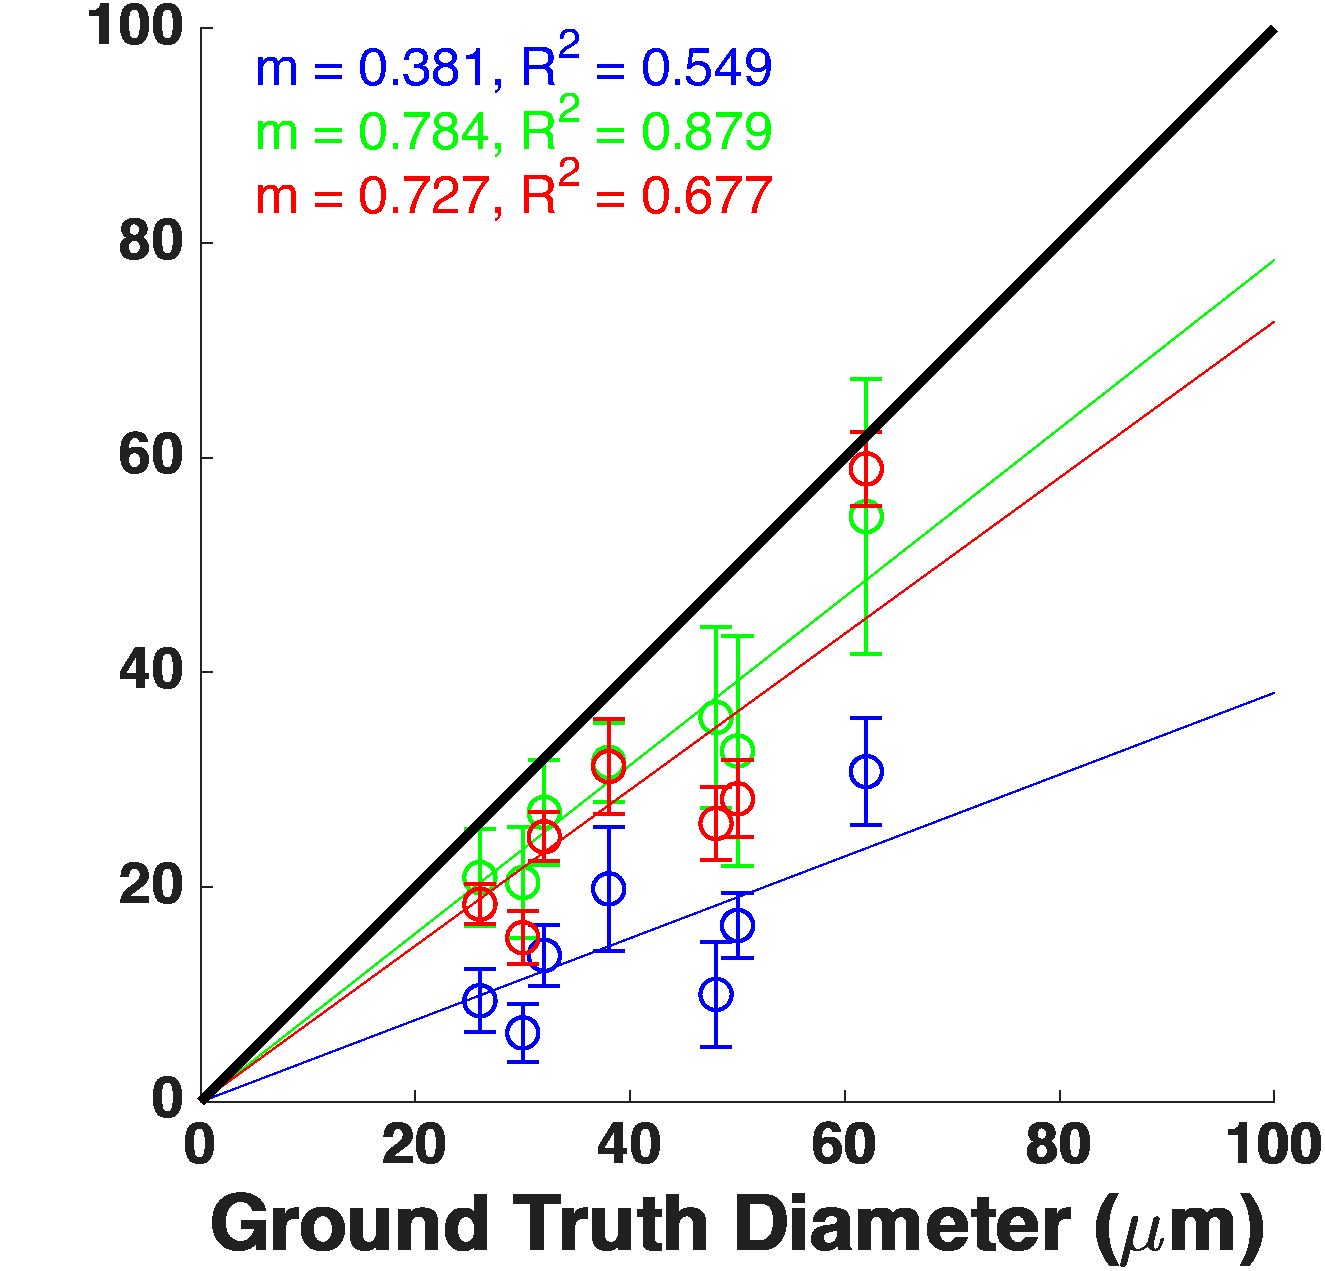
\includegraphics[width=\linewidth]{figures/scatter_bw_mip_c.pdf}\end{subfigure}\\[2pt]
\begin{subfigure}{0.27\linewidth}\centering\captionsetup{margin={3.60mm,0mm}}\caption{MIP, BM-4}\label{fig:scatter_bw_mip_d}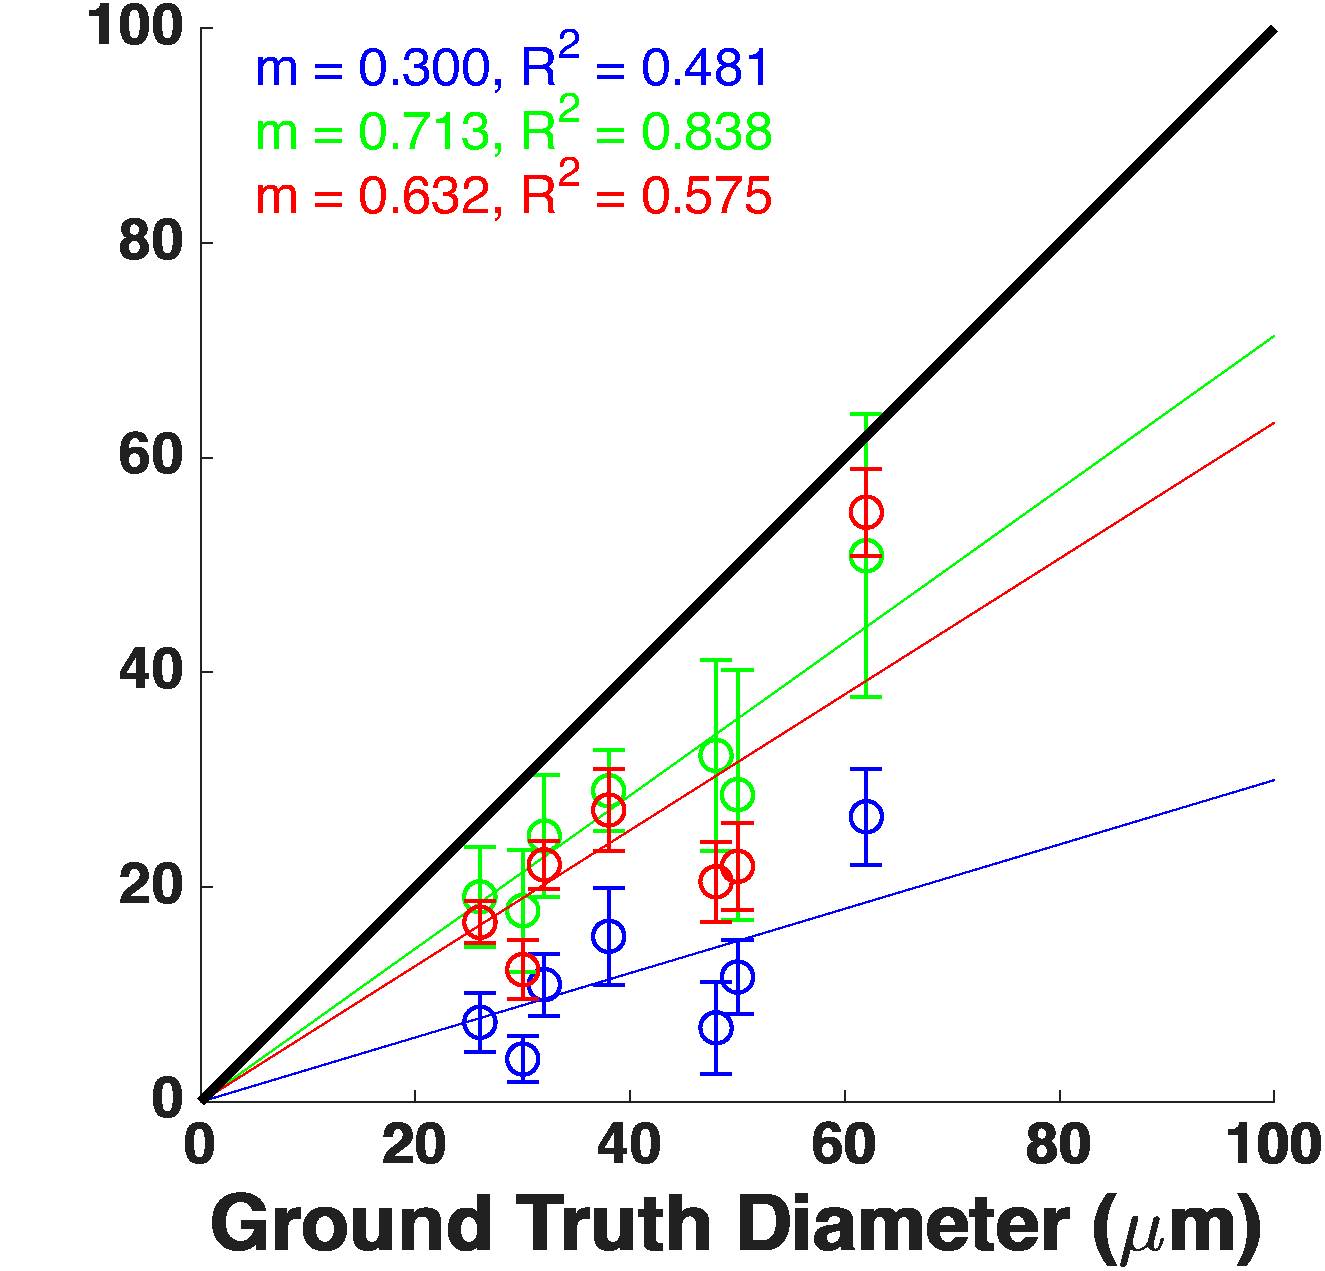
\includegraphics[width=\linewidth]{figures/scatter_bw_mip_d.pdf}\end{subfigure}\hspace{0.05\linewidth}
\begin{subfigure}{0.27\linewidth}\centering\captionsetup{margin={3.60mm,0mm}}\caption{MIP, BM-5}\label{fig:scatter_bw_mip_e}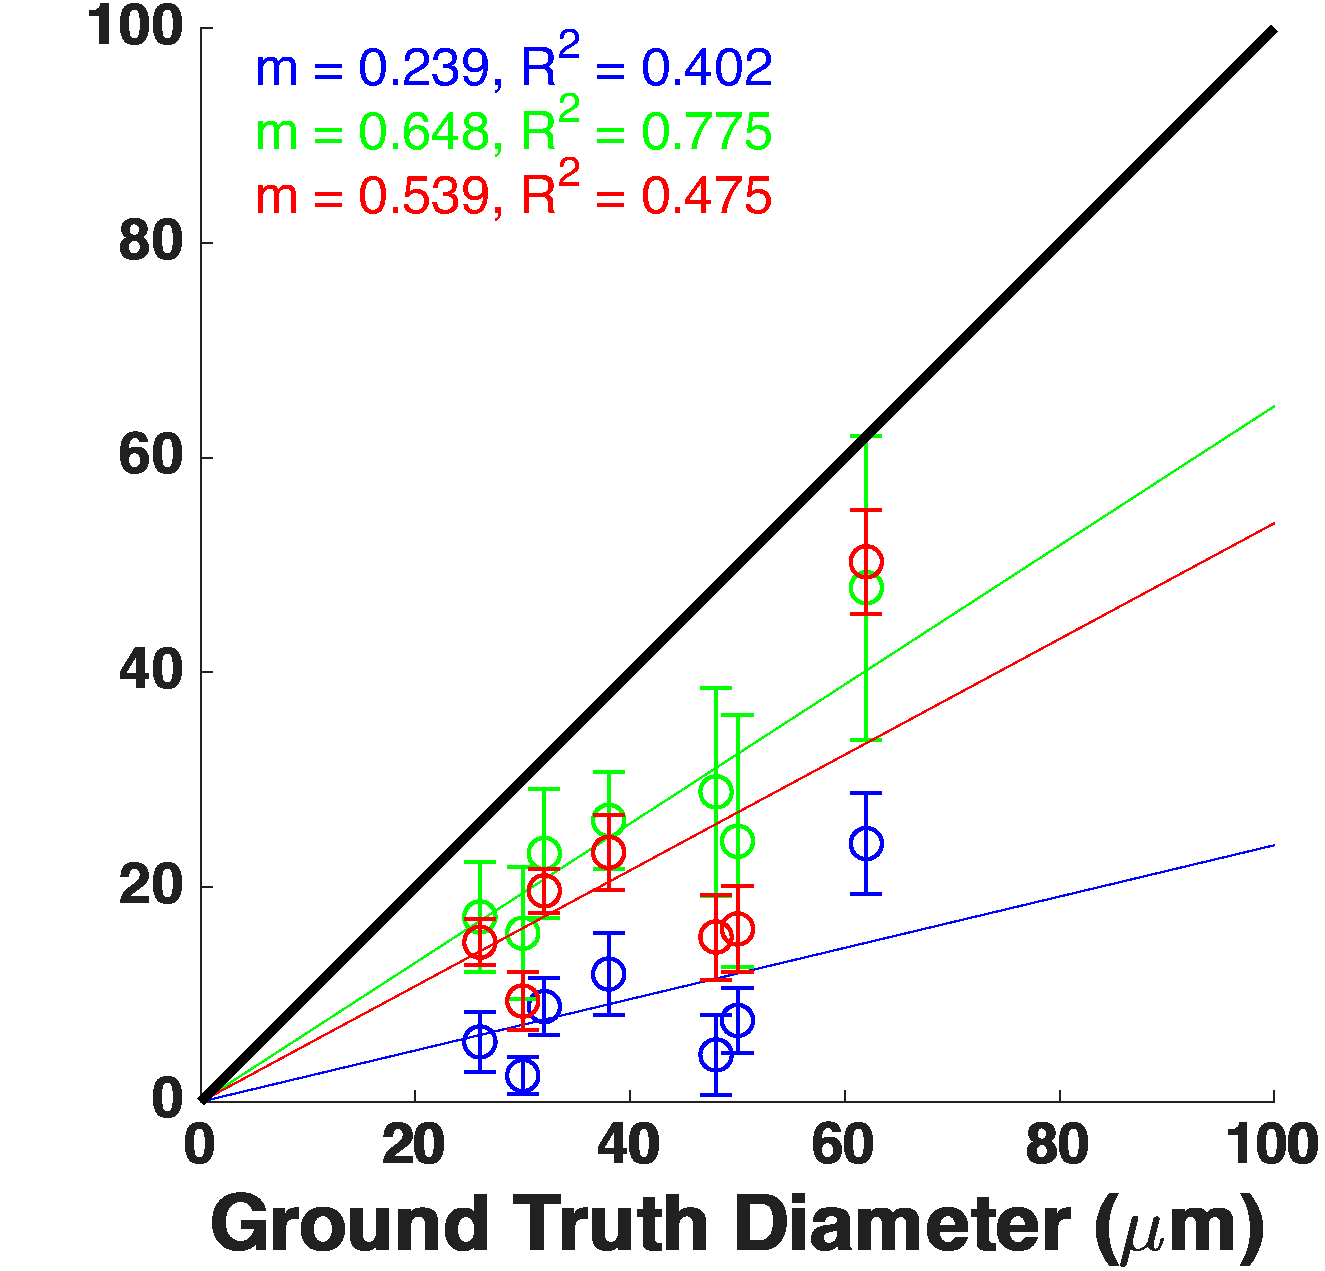
\includegraphics[width=\linewidth]{figures/scatter_bw_mip_e.pdf}\end{subfigure}
\caption{Vessel diameter measured from binarised masks versus ground truth for MIP at five threshold levels: (a) BM-1 through (e) BM-5. Linear regression lines and statistics are shown for pre-contrast (blue), peak contrast (green), and post-contrast (red) conditions.}
\label{fig:scatter_bw_mip}
\end{figure}

\begin{figure}[p]
\centering
\setlength{\abovecaptionskip}{0pt}\setlength{\belowcaptionskip}{2pt}
\captionsetup[subfigure]{position=top,font=bf,skip=2pt}
\begin{subfigure}{0.32\linewidth}\centering\captionsetup{margin={4.20mm,0mm}}\caption{MeIP, BM-1}\label{fig:scatter_bw_meip_a}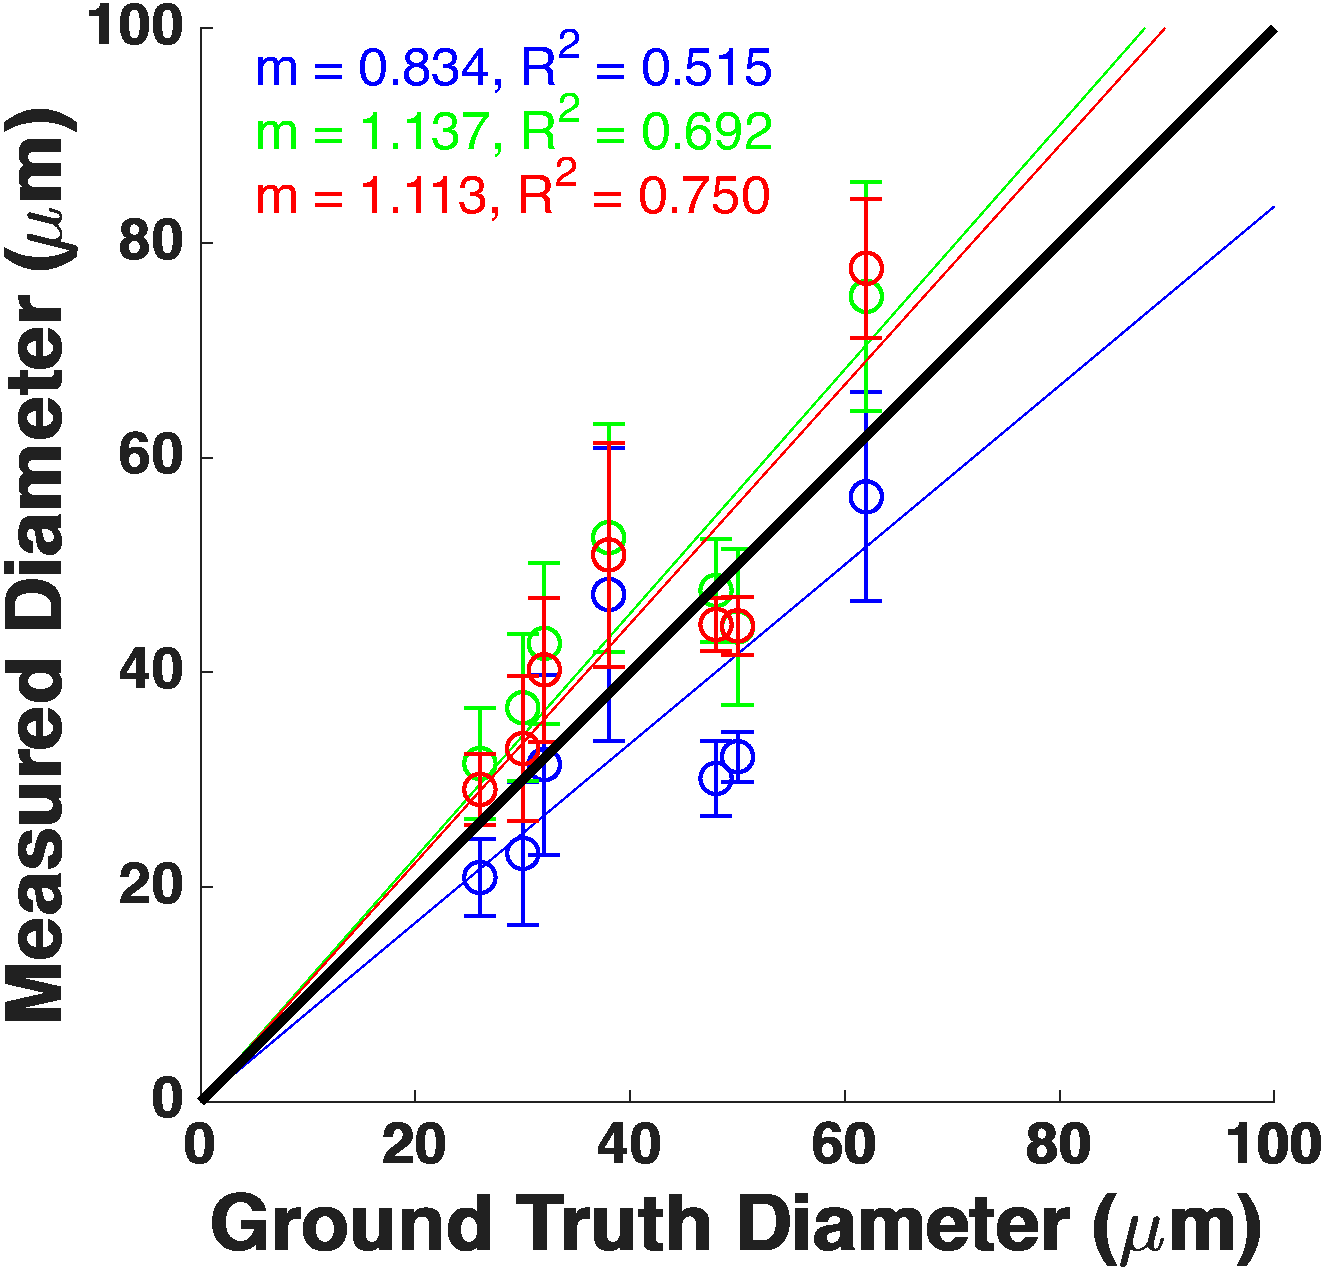
\includegraphics[width=\linewidth]{figures/scatter_bw_meip_a.pdf}\end{subfigure}\hfill
\begin{subfigure}{0.32\linewidth}\centering\captionsetup{margin={4.20mm,0mm}}\caption{MeIP, BM-2}\label{fig:scatter_bw_meip_b}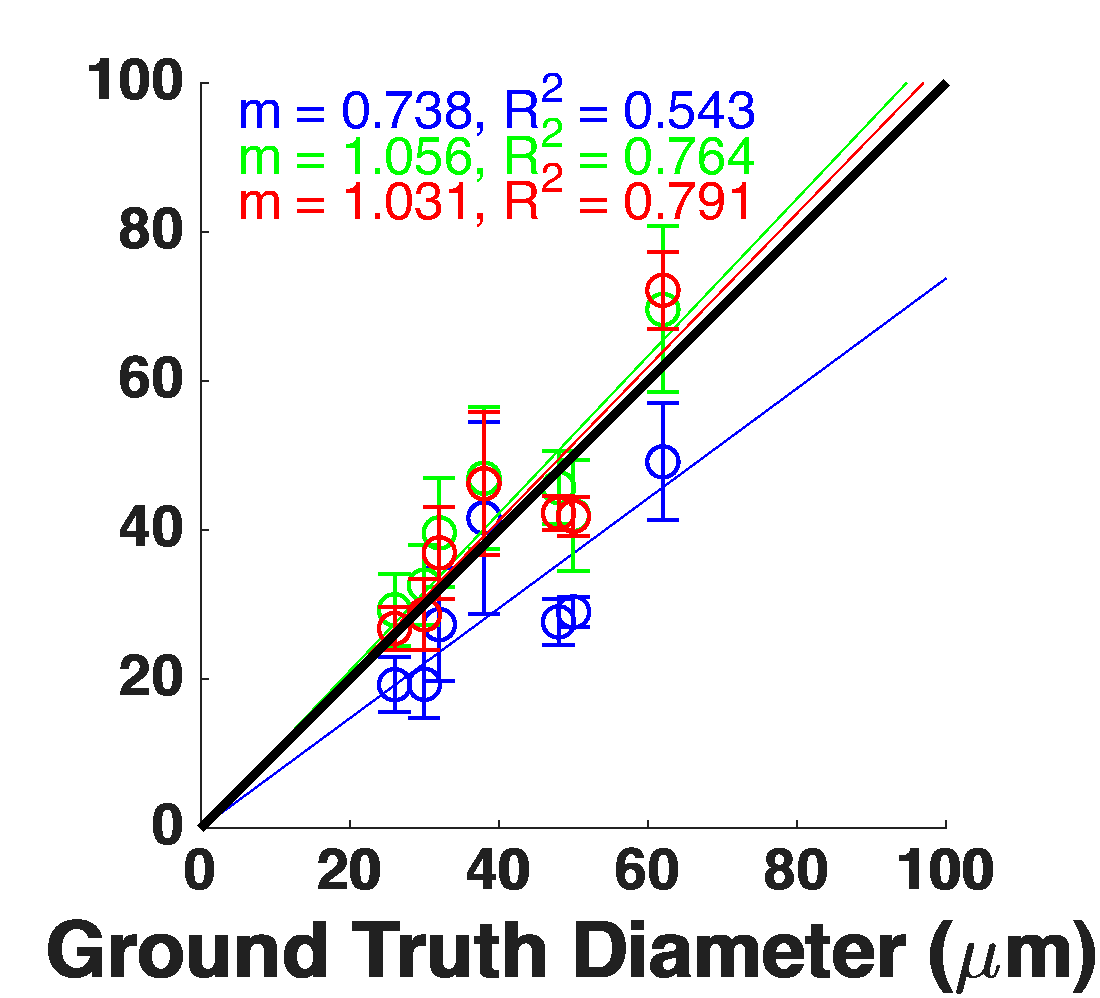
\includegraphics[width=\linewidth]{figures/scatter_bw_meip_b.pdf}\end{subfigure}\hfill
\begin{subfigure}{0.32\linewidth}\centering\captionsetup{margin={4.20mm,0mm}}\caption{MeIP, BM-3}\label{fig:scatter_bw_meip_c}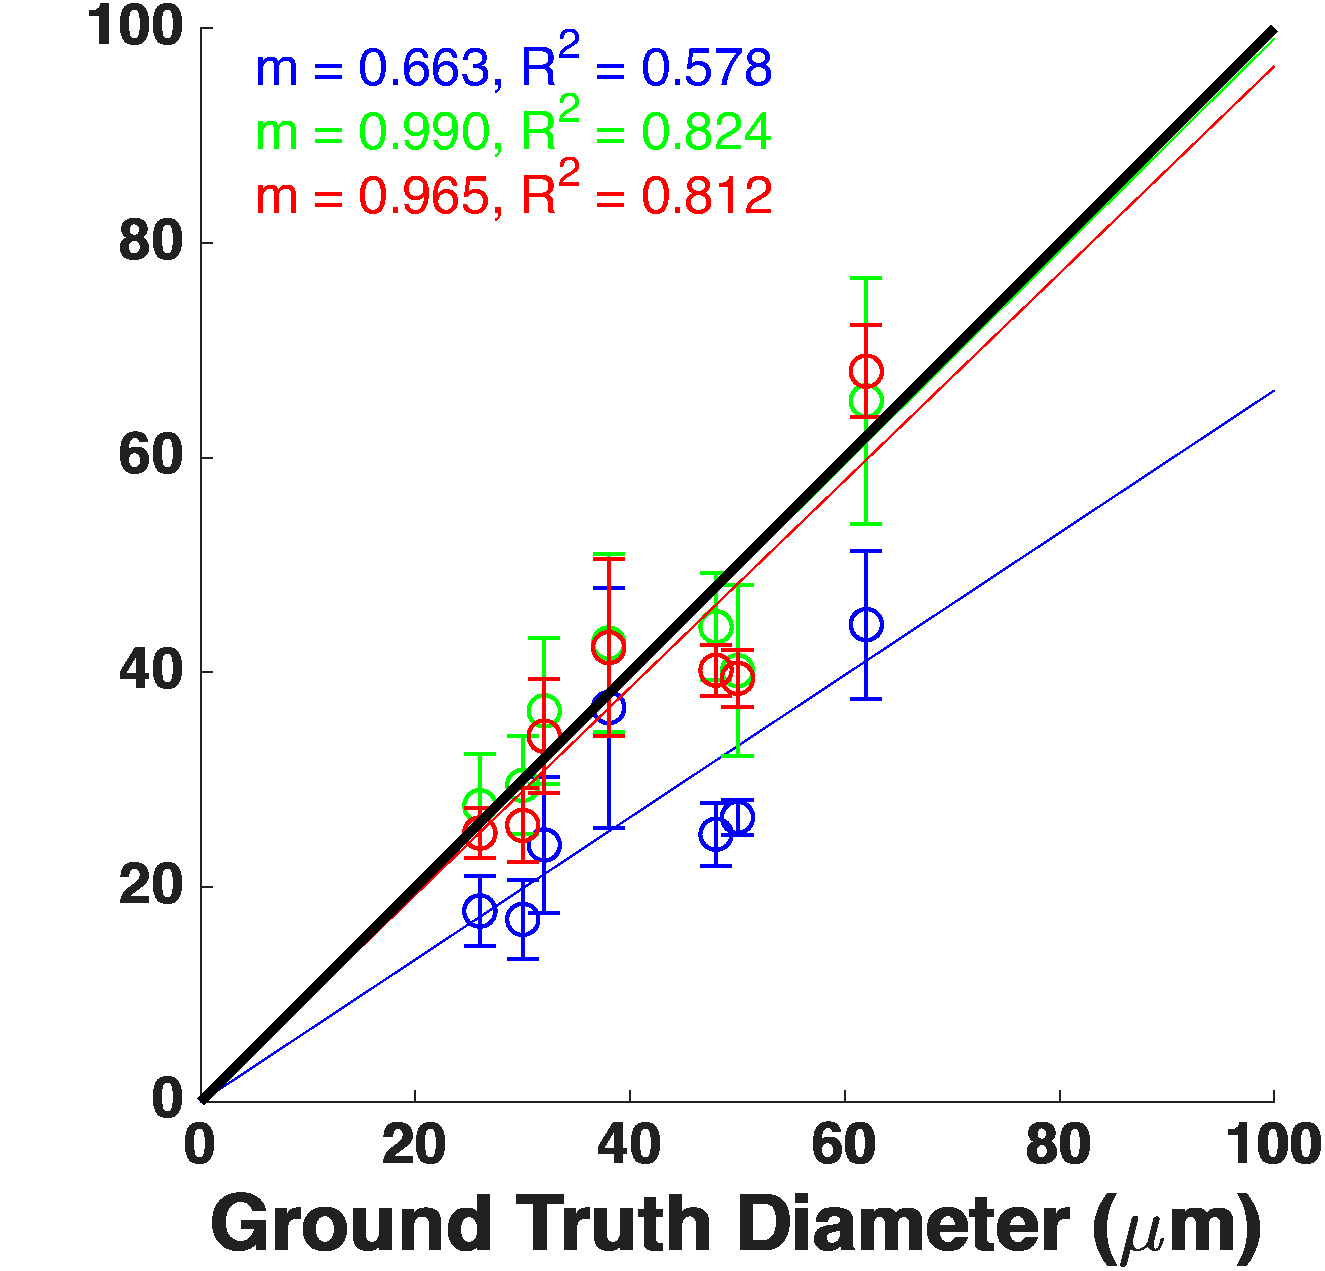
\includegraphics[width=\linewidth]{figures/scatter_bw_meip_c.pdf}\end{subfigure}
\medskip
\begin{subfigure}{0.32\linewidth}\centering\captionsetup{margin={4.20mm,0mm}}\caption{MeIP, BM-4}\label{fig:scatter_bw_meip_d}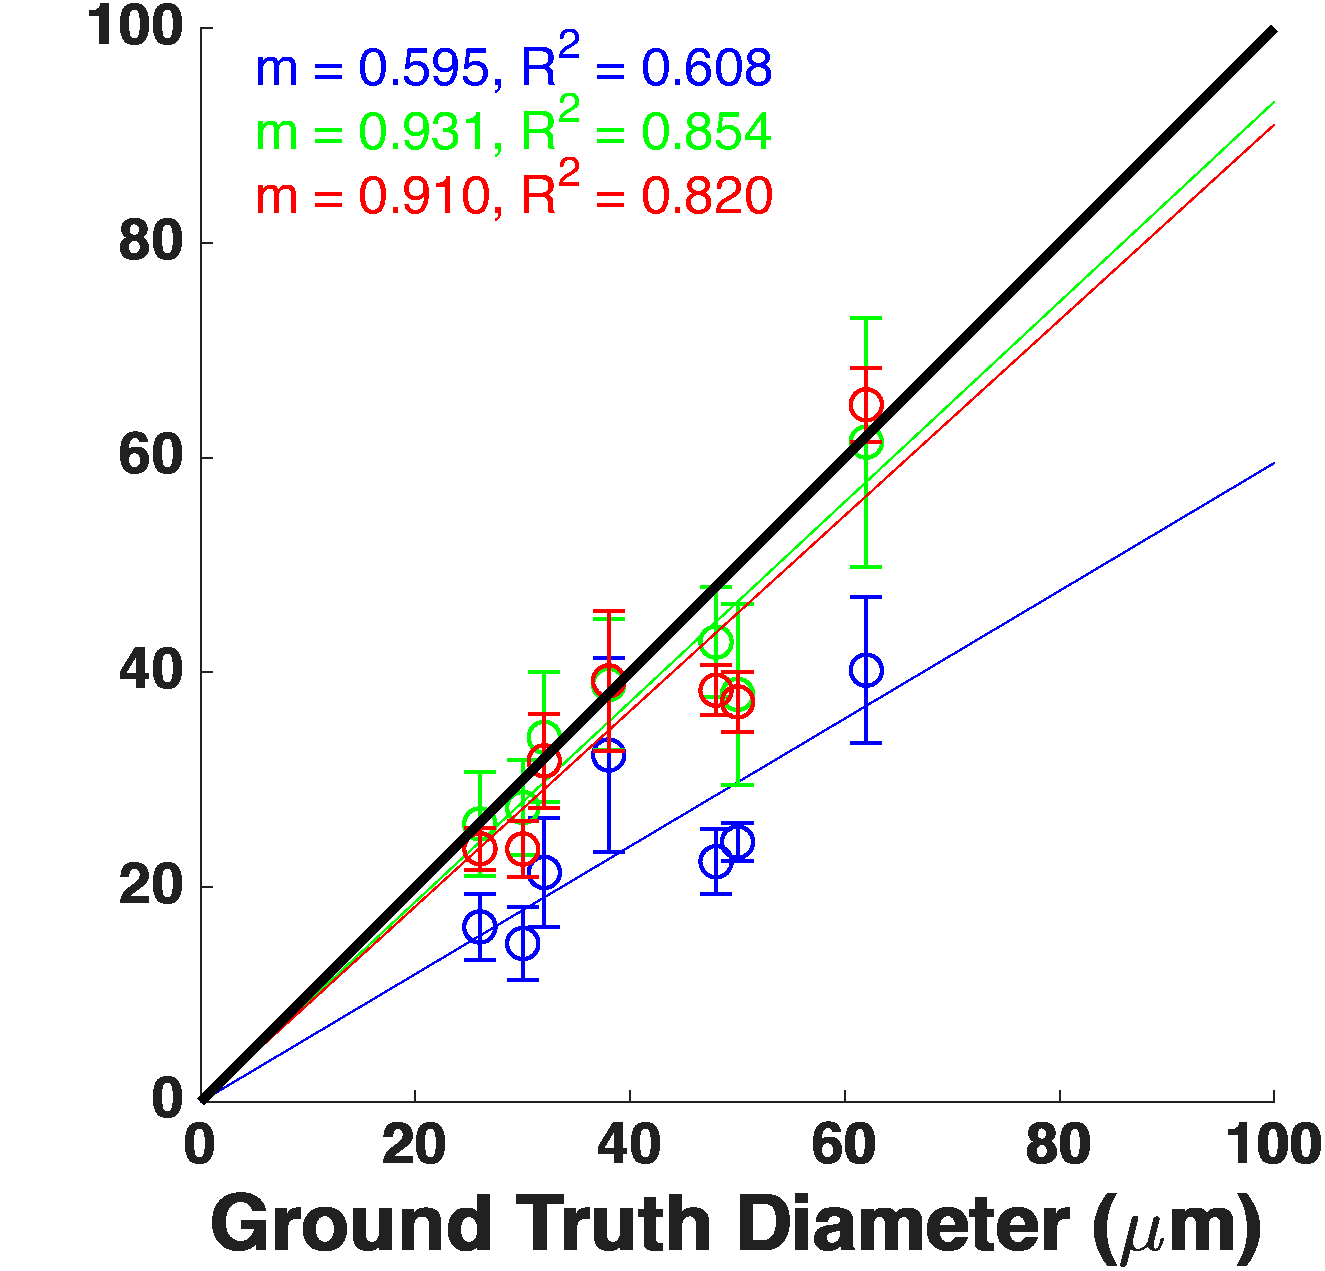
\includegraphics[width=\linewidth]{figures/scatter_bw_meip_d.pdf}\end{subfigure}\hspace{0.02\linewidth}
\begin{subfigure}{0.32\linewidth}\centering\captionsetup{margin={4.20mm,0mm}}\caption{MeIP, BM-5}\label{fig:scatter_bw_meip_e}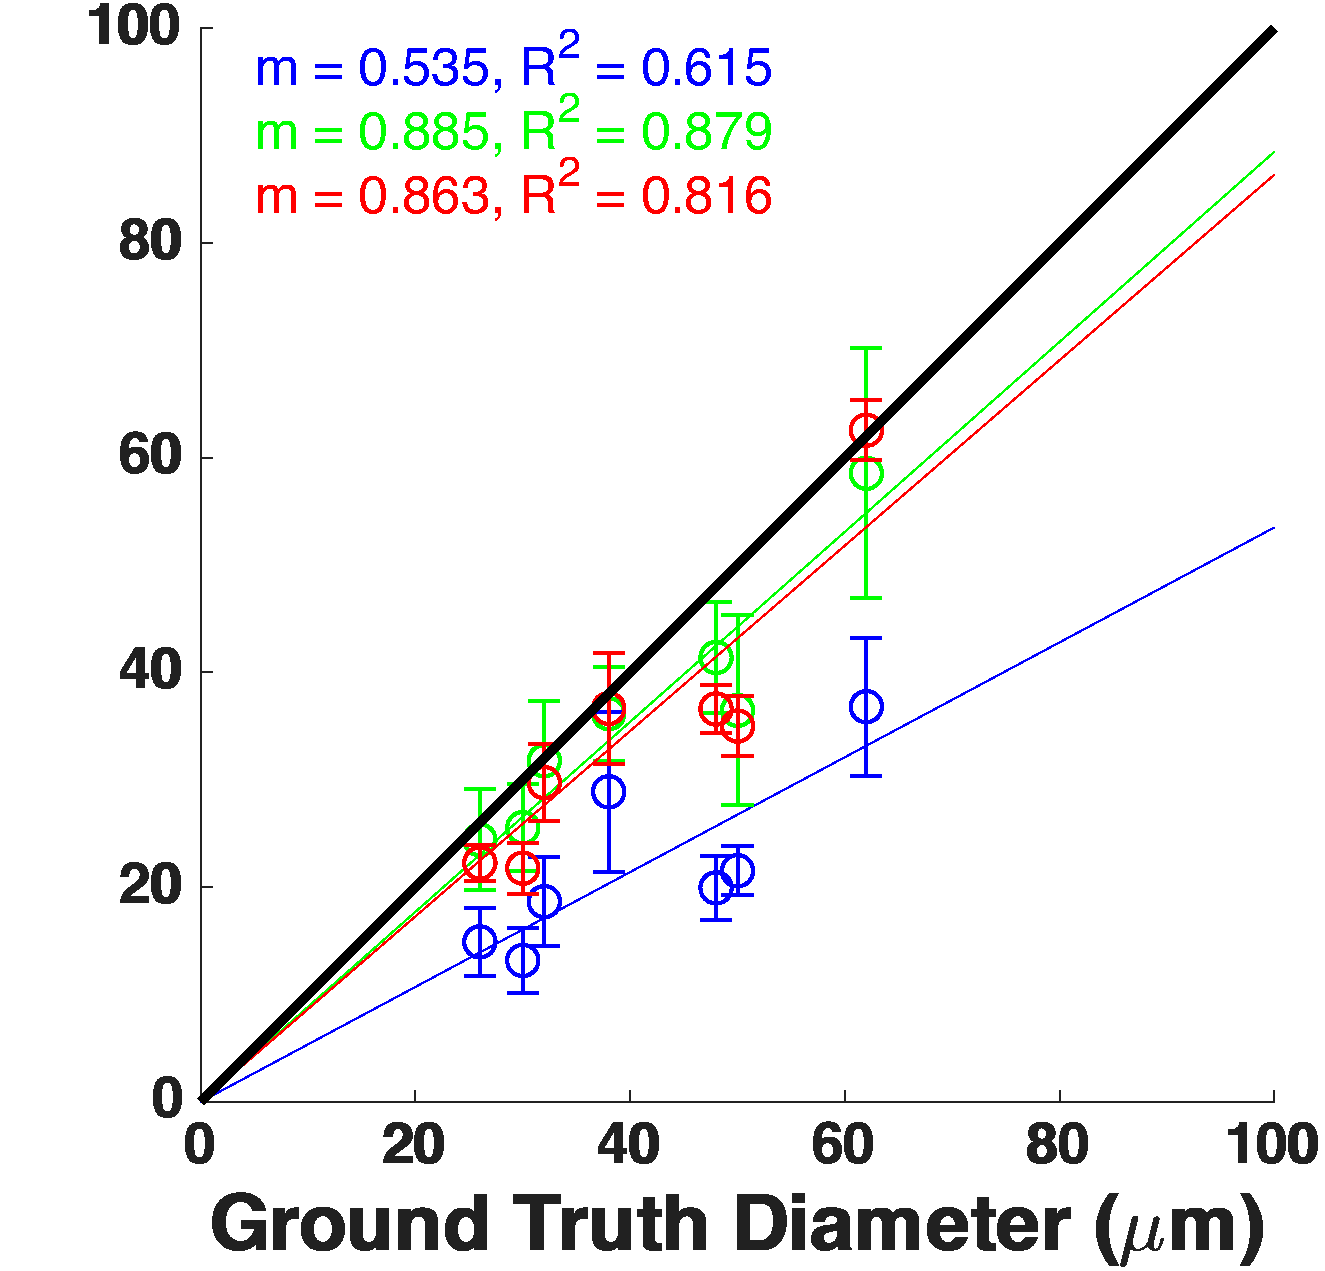
\includegraphics[width=\linewidth]{figures/scatter_bw_meip_e.pdf}\end{subfigure}
\caption{Vessel diameter measured from binarised masks versus ground truth for MeIP at five threshold levels: (a) BM-1 through (e) BM-5. Linear regression lines and statistics are shown for pre-contrast (blue), peak contrast (green), and post-contrast (red) conditions.}
\label{fig:scatter_bw_meip}
\end{figure}

\begin{table}[p]
\setlength{\abovecaptionskip}{4pt}\setlength{\belowcaptionskip}{2pt}
\caption{Summary of slope ($m$), coefficient of determination ($R^2$), and coefficient of variation (CoV) for all diameter measurement methods across pre-contrast, peak contrast, and post-contrast conditions. Methods are grouped as binary-mask-based and model-based. Bold values indicate slope agreement within 10\% of unity ($0.9 \leq m \leq 1.1$), strong linearity ($R^2 \geq 0.90$), or high precision ($\mathrm{CoV} \leq 0.10$).}
\label{tab:accuracy_linearity}
\centering
\resizebox{\textwidth}{!}{%
\begin{tabular}{l c c | c c | c c | c c | c c || c c | c c | c c}
\hline
 & \multicolumn{2}{c|}{\textbf{BM-1}} & \multicolumn{2}{c|}{\textbf{BM-2}} & \multicolumn{2}{c|}{\textbf{BM-3}} & \multicolumn{2}{c|}{\textbf{BM-4}} & \multicolumn{2}{c||}{\textbf{BM-5}} & \multicolumn{2}{c|}{\textbf{$w_{1/e^2,\,\mathrm{G}}$}} & \multicolumn{2}{c|}{\textbf{$w_{fwhm,\,\mathrm{GG}}$}} & \multicolumn{2}{c}{\textbf{$w_{1/e^2,\,\mathrm{GG}}$}} \\
 & MIP & MeIP & MIP & MeIP & MIP & MeIP & MIP & MeIP & MIP & MeIP & MIP & MeIP & MIP & MeIP & MIP & MeIP \\
\hline
\multicolumn{17}{l}{\textit{Slope ($m$)}} \\
\hline
Pre & 0.61 & 0.83 & 0.48 & 0.74 & 0.38 & 0.66 & 0.30 & 0.60 & 0.24 & 0.54 & 0.70 & 0.73 & 0.42 & 0.43 & 0.64 & 0.71 \\
Peak & \textbf{0.96} & 1.14 & 0.86 & \textbf{1.06} & 0.78 & \textbf{0.99} & 0.71 & \textbf{0.93} & 0.65 & 0.89 & 1.15 & \textbf{1.04} & 0.66 & 0.61 & \textbf{0.98} & \textbf{0.98} \\
Post & \textbf{0.92} & 1.11 & 0.82 & \textbf{1.03} & 0.73 & \textbf{0.96} & 0.63 & \textbf{0.91} & 0.54 & 0.86 & 1.12 & \textbf{1.04} & 0.66 & 0.61 & \textbf{1.02} & \textbf{1.00} \\
\hline
\multicolumn{17}{l}{\textit{Coefficient of determination ($R^2$)}} \\
\hline
Pre & 0.62 & 0.51 & 0.60 & 0.54 & 0.55 & 0.58 & 0.48 & 0.61 & 0.40 & 0.62 & 0.73 & 0.63 & 0.67 & 0.55 & 0.81 & 0.76 \\
Peak & 0.88 & 0.69 & \textbf{0.90} & 0.76 & 0.88 & 0.82 & 0.84 & 0.85 & 0.78 & 0.88 & \textbf{0.90} & \textbf{0.95} & \textbf{0.95} & \textbf{0.94} & \textbf{0.98} & \textbf{0.97} \\
Post & 0.81 & 0.75 & 0.76 & 0.79 & 0.68 & 0.81 & 0.58 & 0.82 & 0.48 & 0.82 & \textbf{0.92} & \textbf{0.98} & \textbf{0.96} & \textbf{0.98} & \textbf{0.95} & \textbf{0.97} \\
\hline
\multicolumn{17}{l}{\textit{Coefficient of variation (CoV)}} \\
\hline
Pre & 0.20 & 0.20 & 0.24 & 0.19 & 0.30 & 0.19 & 0.37 & 0.19 & 0.47 & 0.19 & 0.26 & 0.14 & 0.27 & 0.15 & 0.25 & 0.13 \\
Peak & 0.17 & 0.16 & 0.20 & 0.17 & 0.22 & 0.17 & 0.27 & 0.17 & 0.32 & 0.17 & 0.24 & 0.15 & 0.23 & 0.16 & 0.21 & 0.14 \\
Post & \textbf{0.10} & 0.13 & \textbf{0.10} & 0.12 & 0.12 & 0.11 & 0.15 & \textbf{0.10} & 0.18 & \textbf{0.09} & 0.18 & \textbf{0.10} & 0.18 & 0.11 & 0.16 & \textbf{0.09} \\
\hline
\end{tabular}%
}
\end{table}

The $w_{1/e^2,\,\mathrm{G}}$ with MIP slightly overestimated at both peak and post-contrast ($m = 1.15$ and $m = 1.12$), while MeIP yielded values closer to unity ($m = 1.04$ in both conditions). The $w_{1/e^2,\,\mathrm{GG}}$ with MeIP provided the best overall agreement, achieving a slope closest to unity with $m = 1.001$ ($R^2 = 0.97$) post-contrast, which was the closest to the identity line of all tested model-based methods. MeIP generally gave slopes closer to unity than MIP, and also provided smaller standard deviations for the model-based methods (Fig.~\ref{fig:scatter_model}). Pre-contrast $R^2$ was higher for MIP across all three metrics, and MeIP only surpassed MIP post-contrast (Table~\ref{tab:accuracy_linearity}, Fig.~\ref{fig:scatter_model}).

For binary-mask-based methods, the slope decreased with increasing threshold across all contrast conditions and projections (Fig.~\ref{fig:scatter_bw_mip}, Fig.~\ref{fig:scatter_bw_meip}) (Table~\ref{tab:accuracy_linearity}). MeIP slopes were consistently higher than MIP at every threshold and contrast condition, though at lower thresholds and at peak and post-contrast, MeIP tended to slightly overestimate vessel diameter.~The $R^2$ values showed opposite trends for the two projections, which are most directly compared in the summary bar plots of Fig.~\ref{fig:cov_r2}c,d. For MIP, $R^2$ decreased with increasing threshold across all contrast conditions, most strongly post-contrast (Fig.~\ref{fig:cov_r2}c). For MeIP, $R^2$ instead increased with threshold, most evident at peak contrast (Fig.~\ref{fig:cov_r2}d). Overall, MeIP provided more accurate binary-mask-based diameter measurements than MIP at most thresholds, and was more linear at the higher thresholds. The exception was the lowest threshold, where MIP stayed closer to the identity line at peak and post-contrast ($m = 0.96$ and $m = 0.92$, against $m = 1.14$ and $m = 1.11$ for MeIP), and was also more linear (Fig.~\ref{fig:scatter_bw_mip}a, Fig.~\ref{fig:scatter_bw_meip}a).

The precision of each method was assessed via the CoV (Table~\ref{tab:accuracy_linearity}, Fig.~\ref{fig:cov_r2}a,b). For MIP, the binary-mask-based CoV increased substantially with threshold, whereas the model-based CoV remained stable across all contrast conditions. For MeIP, the binary-mask-based CoV was notably more stable across thresholds than for MIP, and the model-based CoV values were lower overall, though they increased slightly at peak contrast before decreasing post-contrast. Across both methods, MeIP yielded lower CoV values than MIP pre-contrast and more stable values post-contrast.

Among the model-based metrics, $w_{fwhm,\,\mathrm{GG}}$ showed the largest underestimation in all three contrast conditions, with slopes between 0.42 and 0.66 across both projections. Its linearity was not correspondingly poor, however, post-contrast it reached $R^2 = 0.96$ for MIP and $R^2 = 0.98$ for MeIP, the highest and joint-highest of the model-based metrics respectively, and its precision remained comparable to the other model metrics. Overall, model-based methods outperformed binary-mask-based methods in both accuracy and precision, with two exceptions. At the two lowest MIP thresholds the binary-mask-based CoV was lower than that of any model-based metric (0.10 at BM-1 and BM-2 post-contrast, against 0.16--0.18), so MIP was more precise there but less linear ($R^2 = 0.81$ against 0.92--0.96). At the higher MeIP thresholds precision was comparable to the model-based methods, though accuracy was lower.

\begin{figure}[htbp]
\centering
\setlength{\abovecaptionskip}{0pt}\setlength{\belowcaptionskip}{2pt}
\captionsetup[subfigure]{position=top,font=bf,skip=2pt}
\begin{subfigure}{0.48\linewidth}\centering\captionsetup{margin={5.25mm,0mm}}\caption{MIP, CoV}\label{fig:cov_r2_a}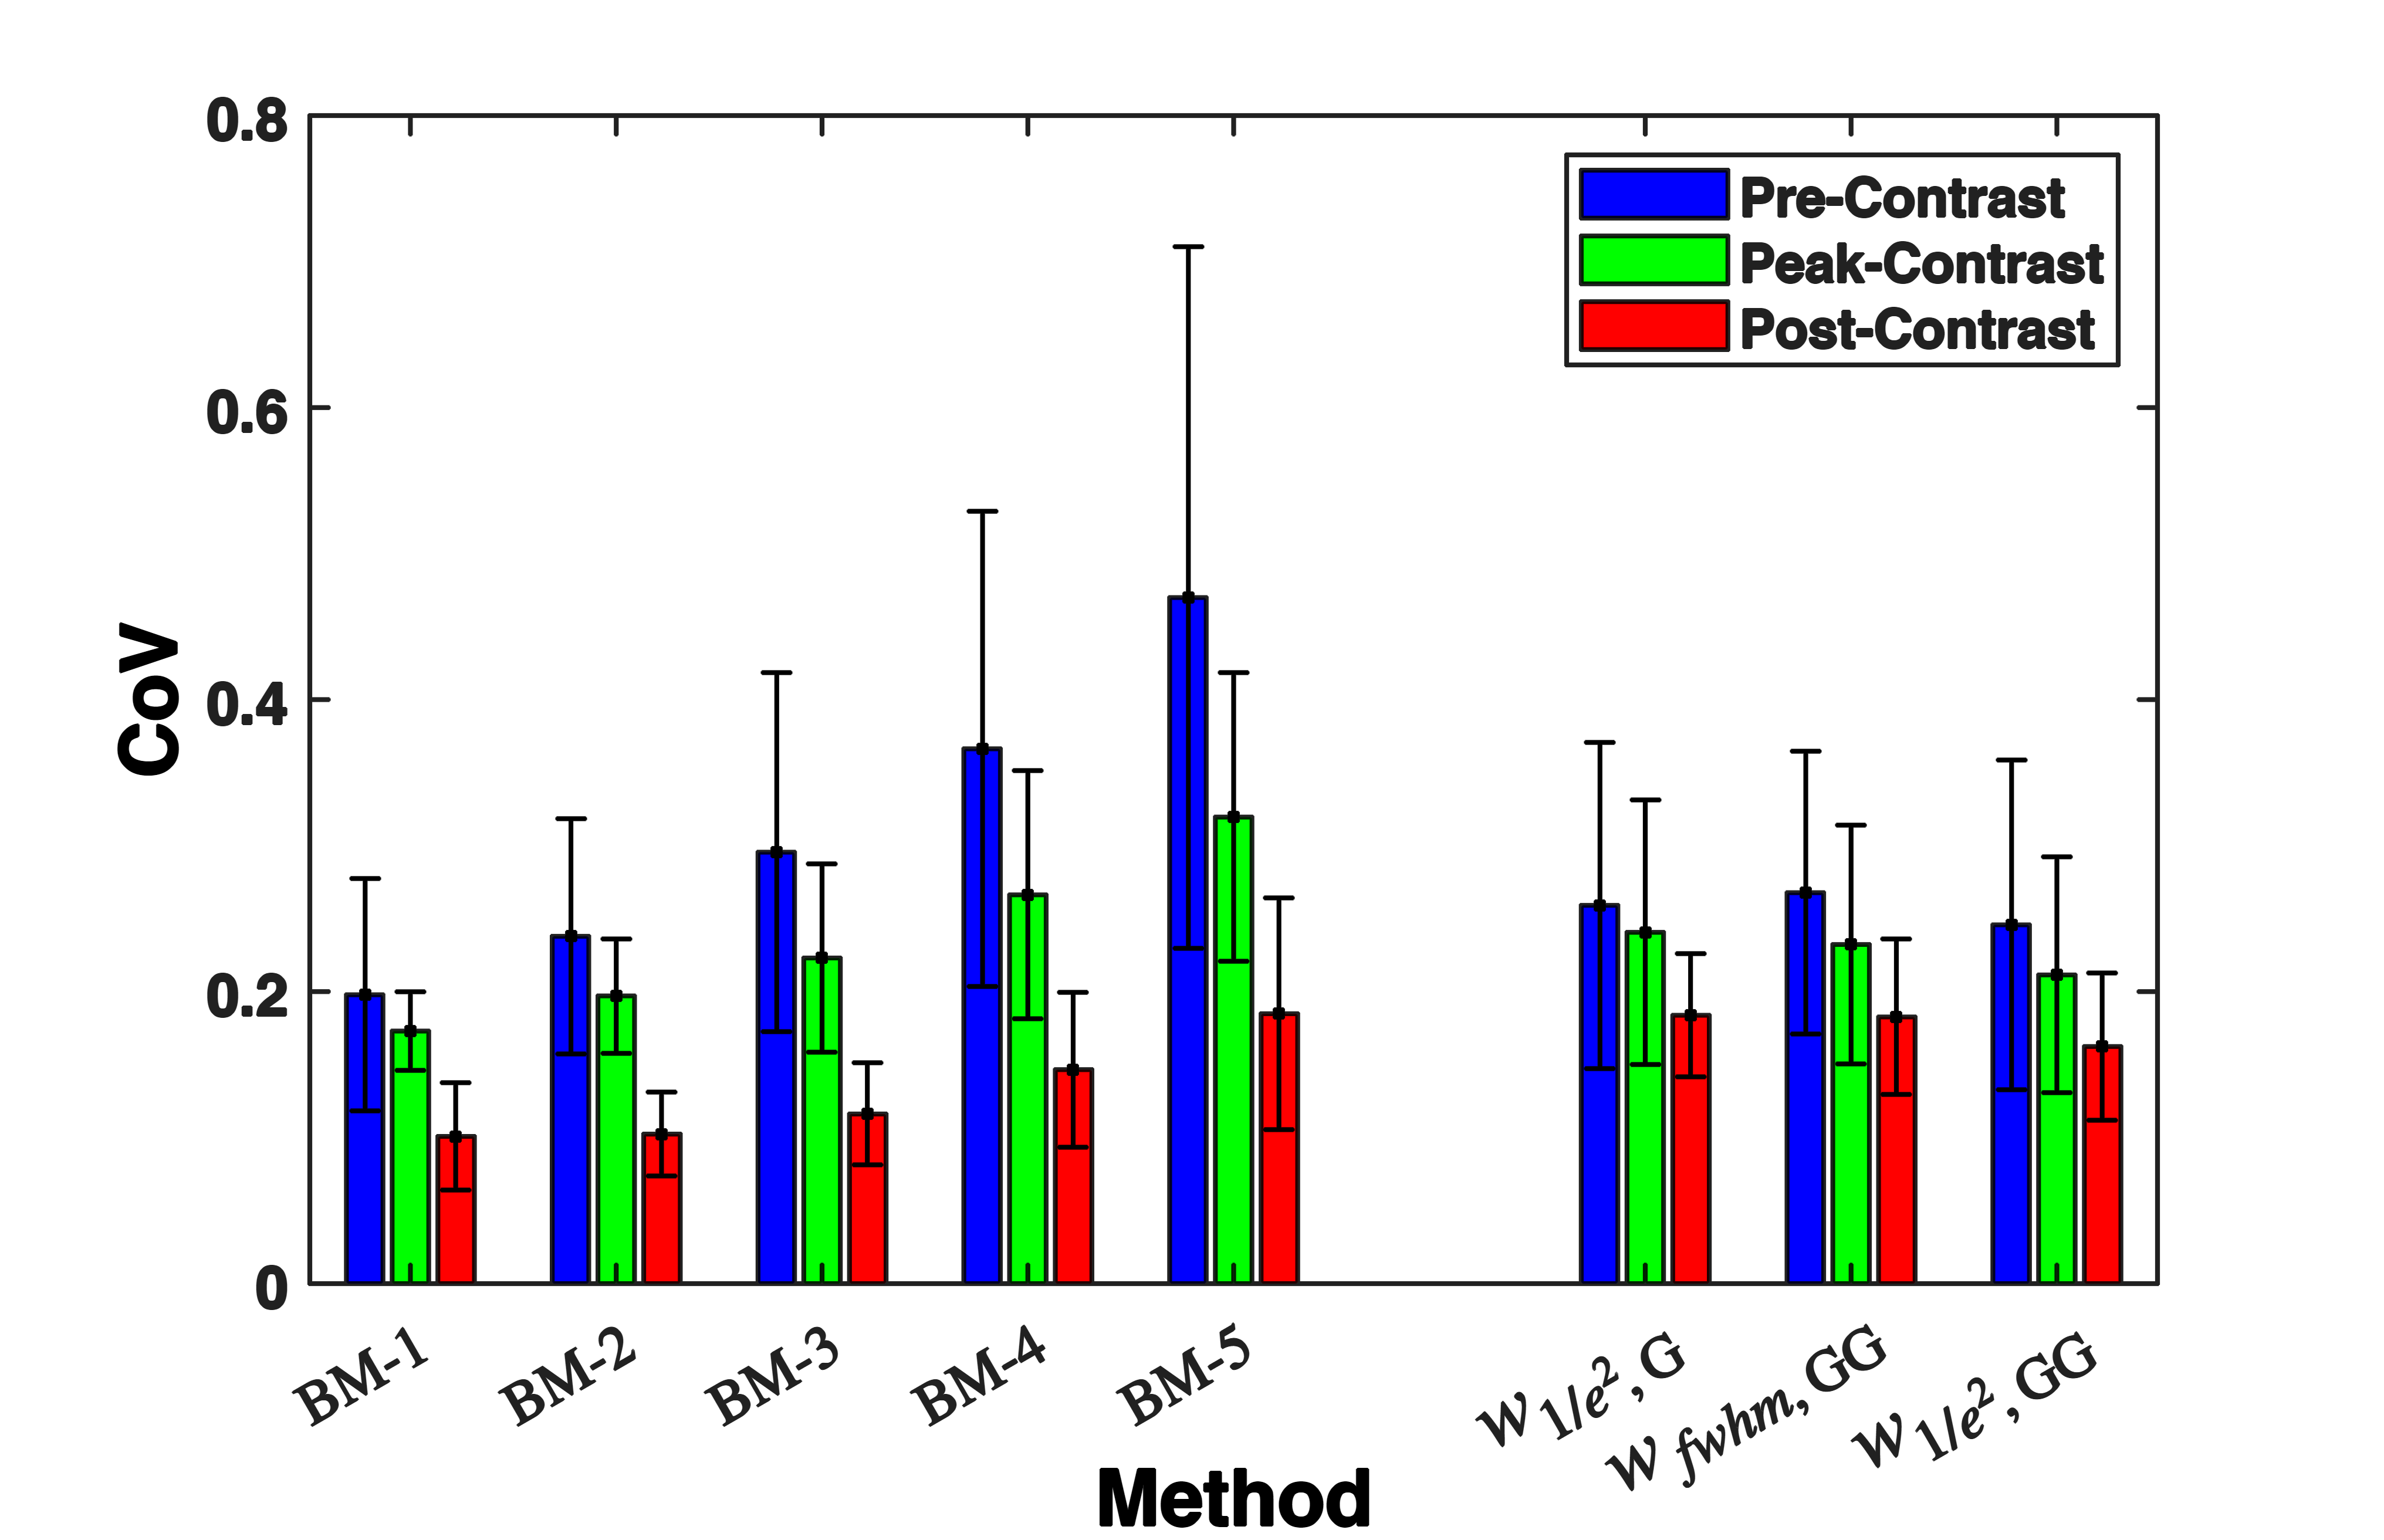
\includegraphics[width=\linewidth,trim=148 0 361 145,clip]{figures/cov_r2_a.png}\end{subfigure}\hfill
\begin{subfigure}{0.48\linewidth}\centering\captionsetup{margin={5.25mm,0mm}}\caption{MeIP, CoV}\label{fig:cov_r2_b}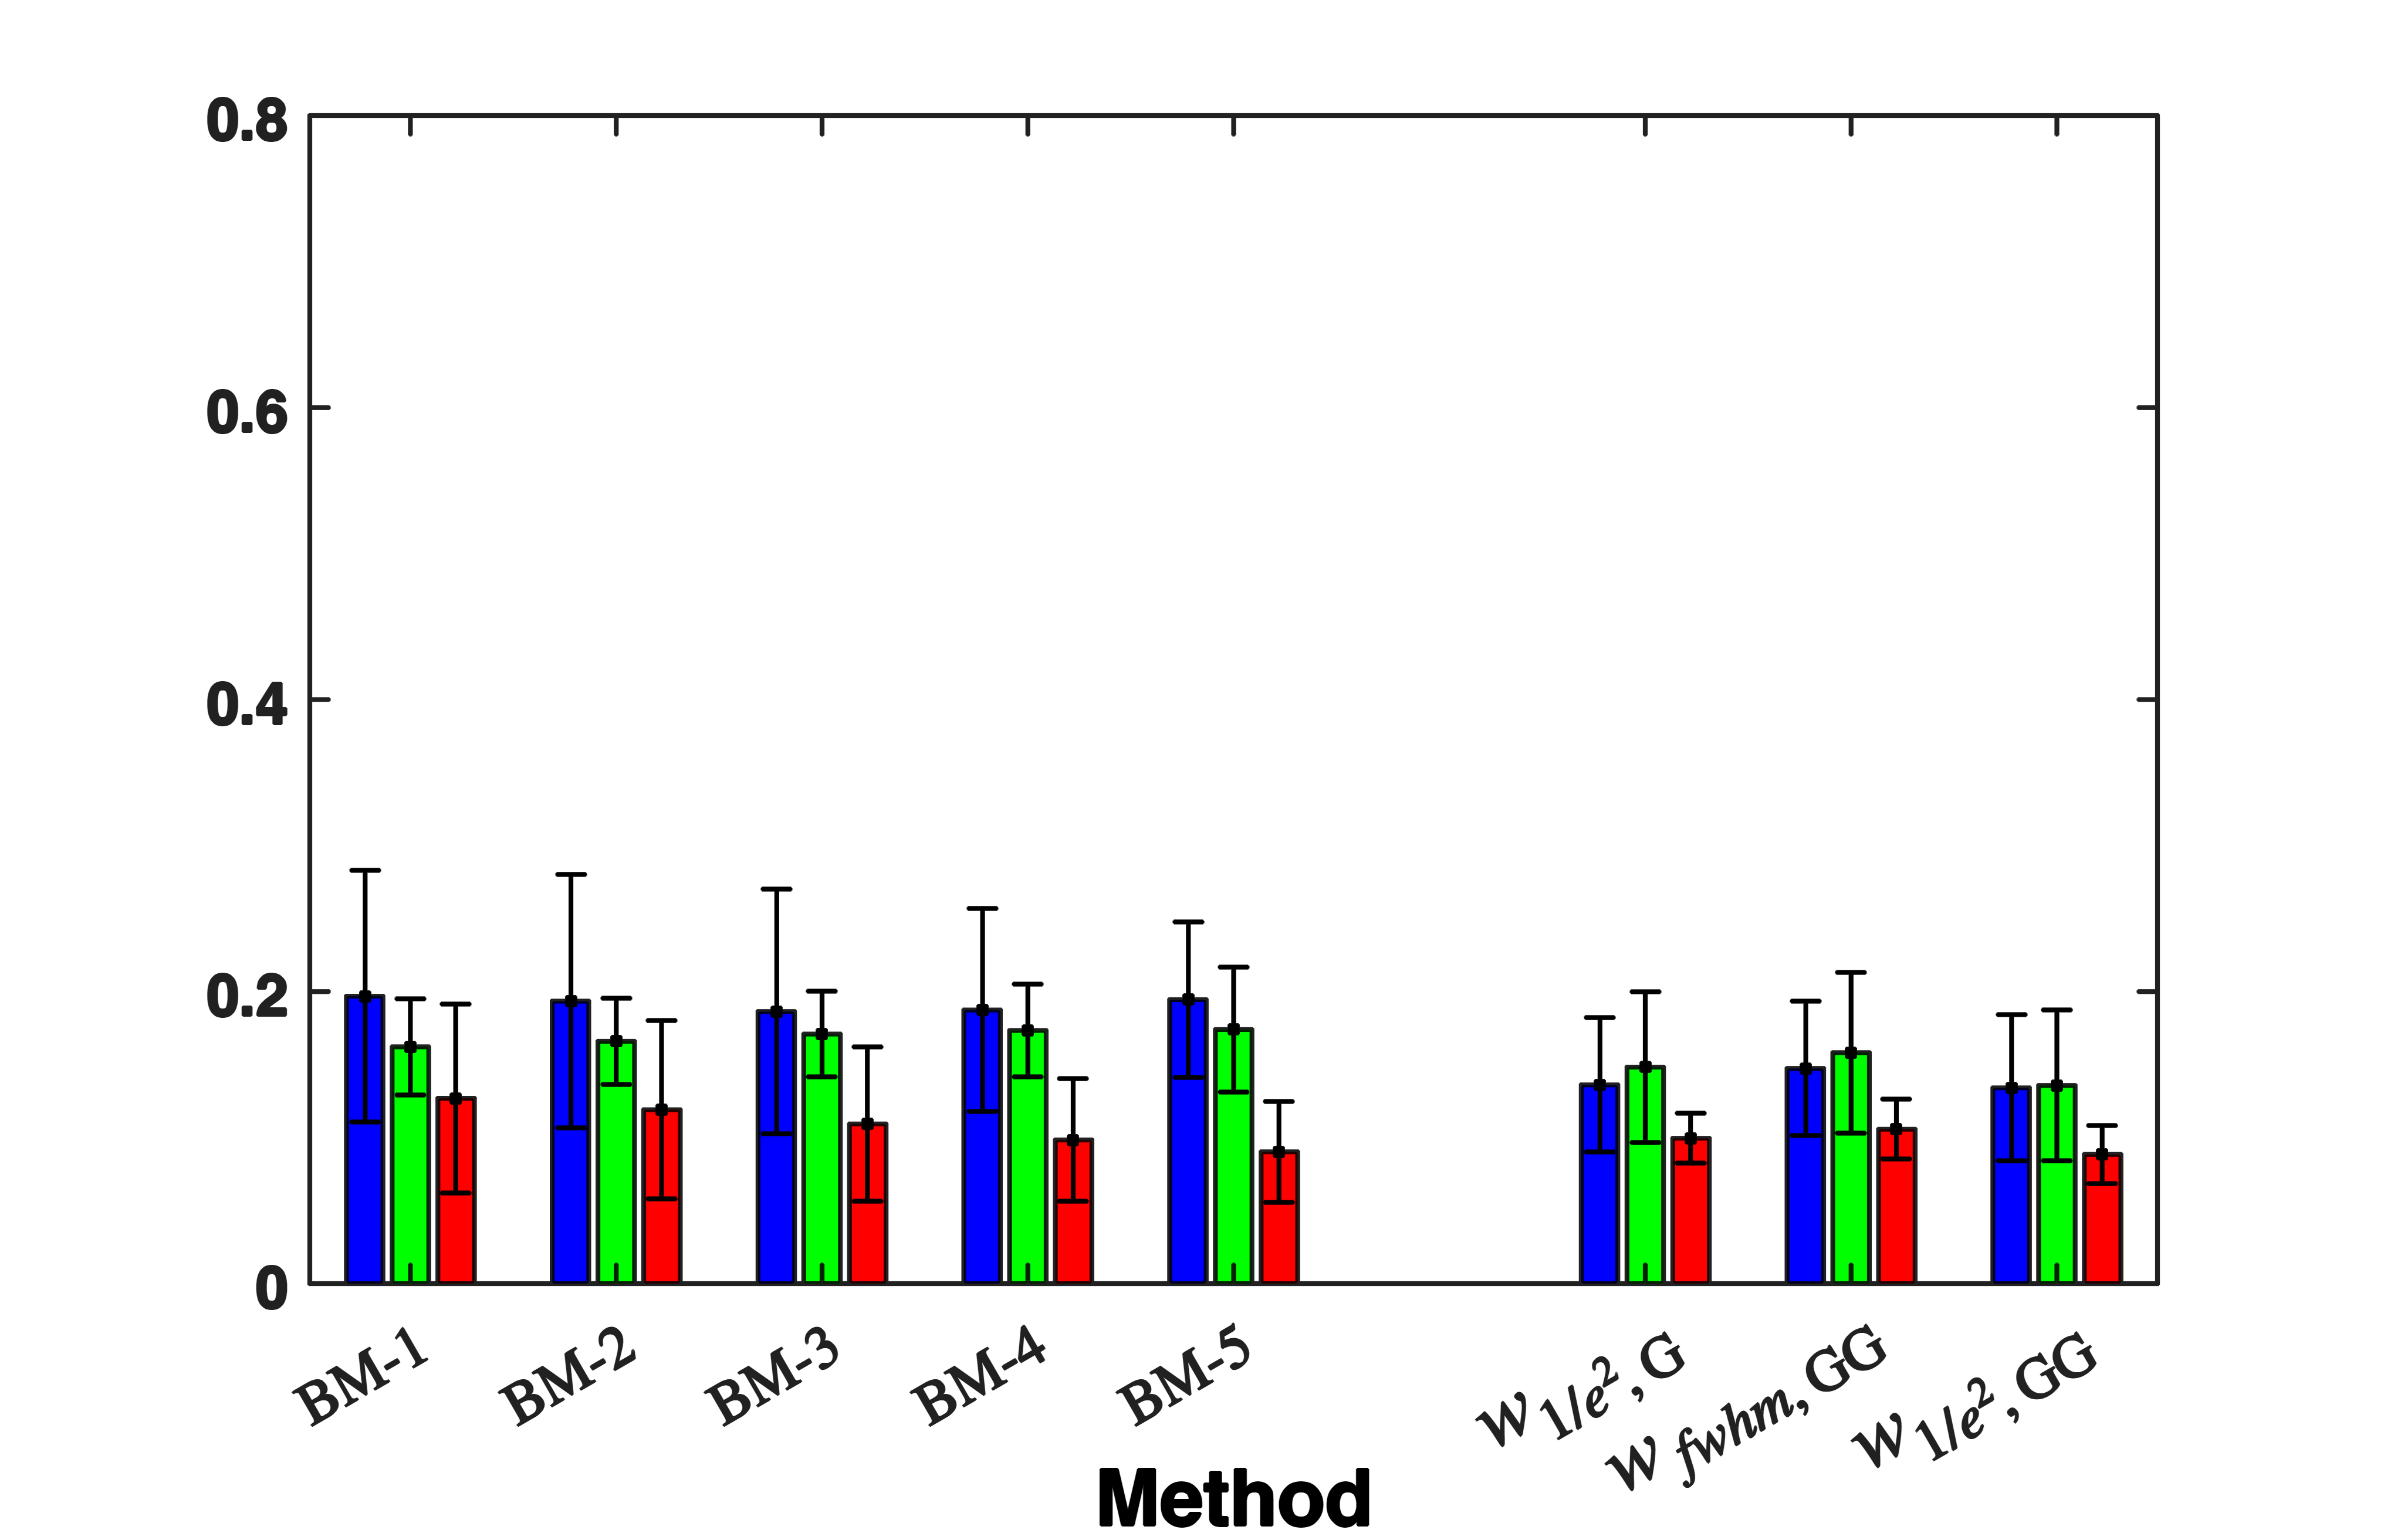
\includegraphics[width=\linewidth,trim=148 0 361 145,clip]{figures/cov_r2_b.png}\end{subfigure}
\medskip
\begin{subfigure}{0.48\linewidth}\centering\captionsetup{margin={5.75mm,0mm}}\caption{MIP, $R^2$}\label{fig:cov_r2_c}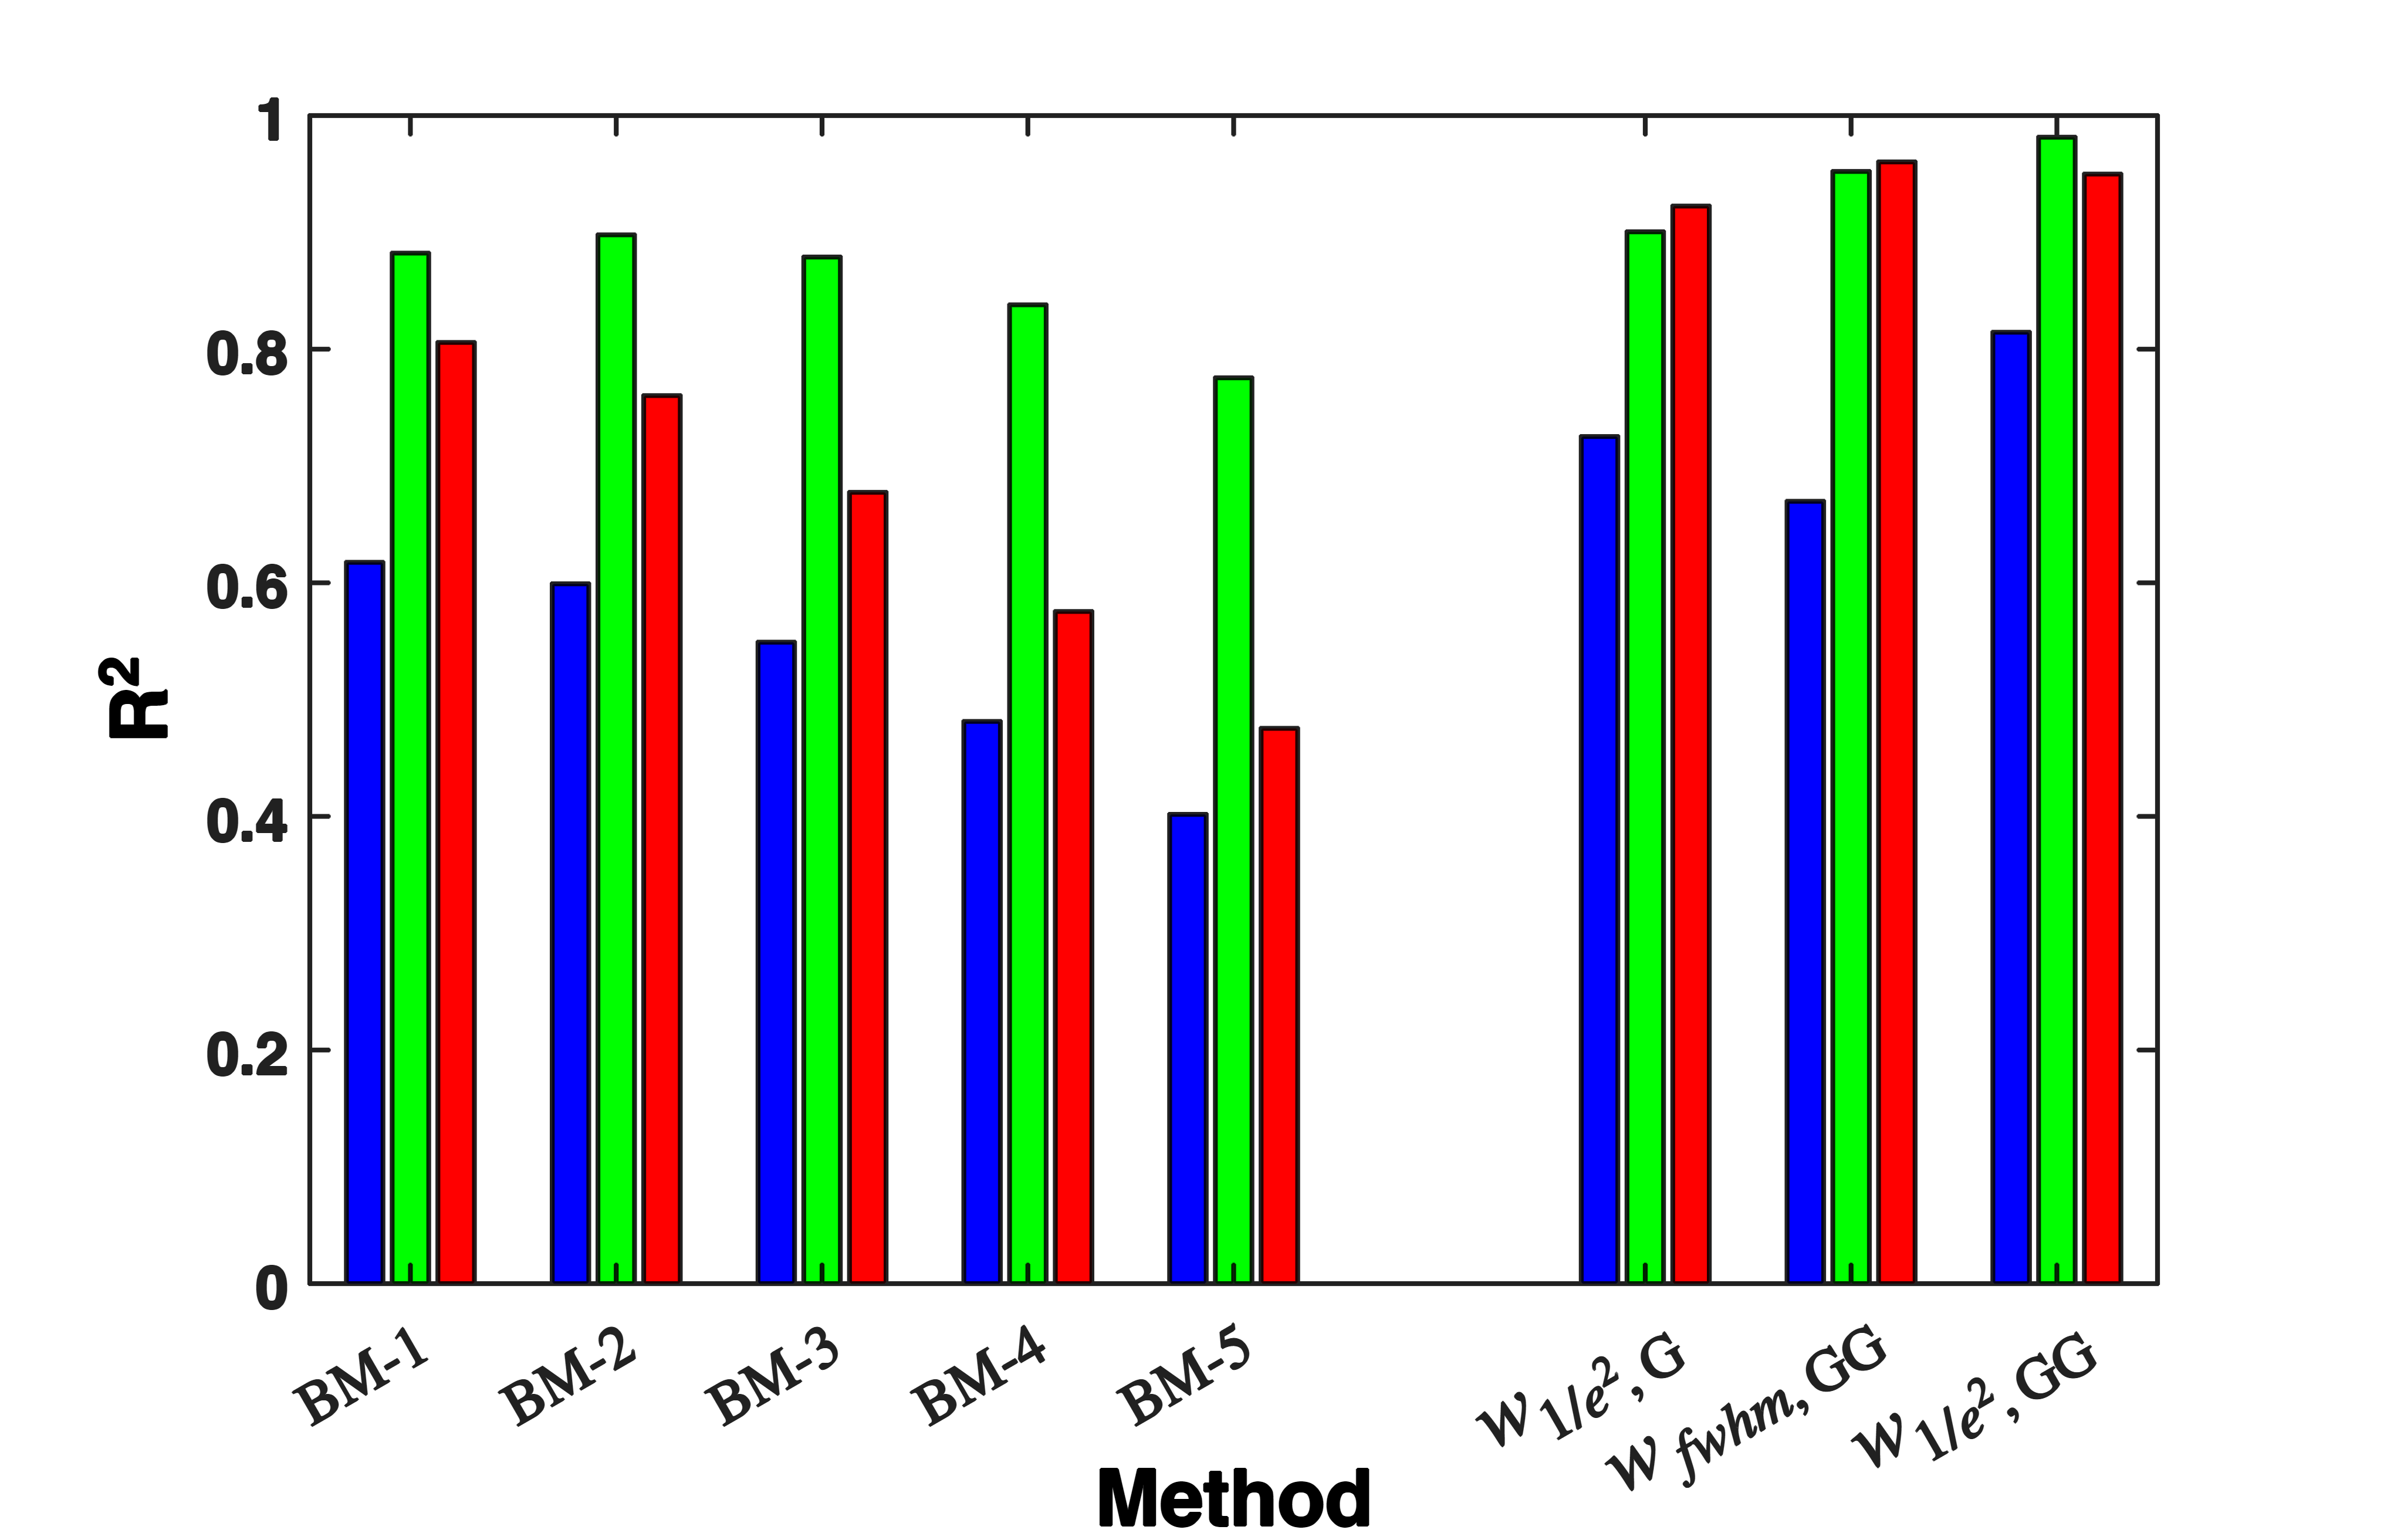
\includegraphics[width=\linewidth,trim=148 0 361 145,clip]{figures/cov_r2_c.png}\end{subfigure}\hfill
\begin{subfigure}{0.48\linewidth}\centering\captionsetup{margin={5.75mm,0mm}}\caption{MeIP, $R^2$}\label{fig:cov_r2_d}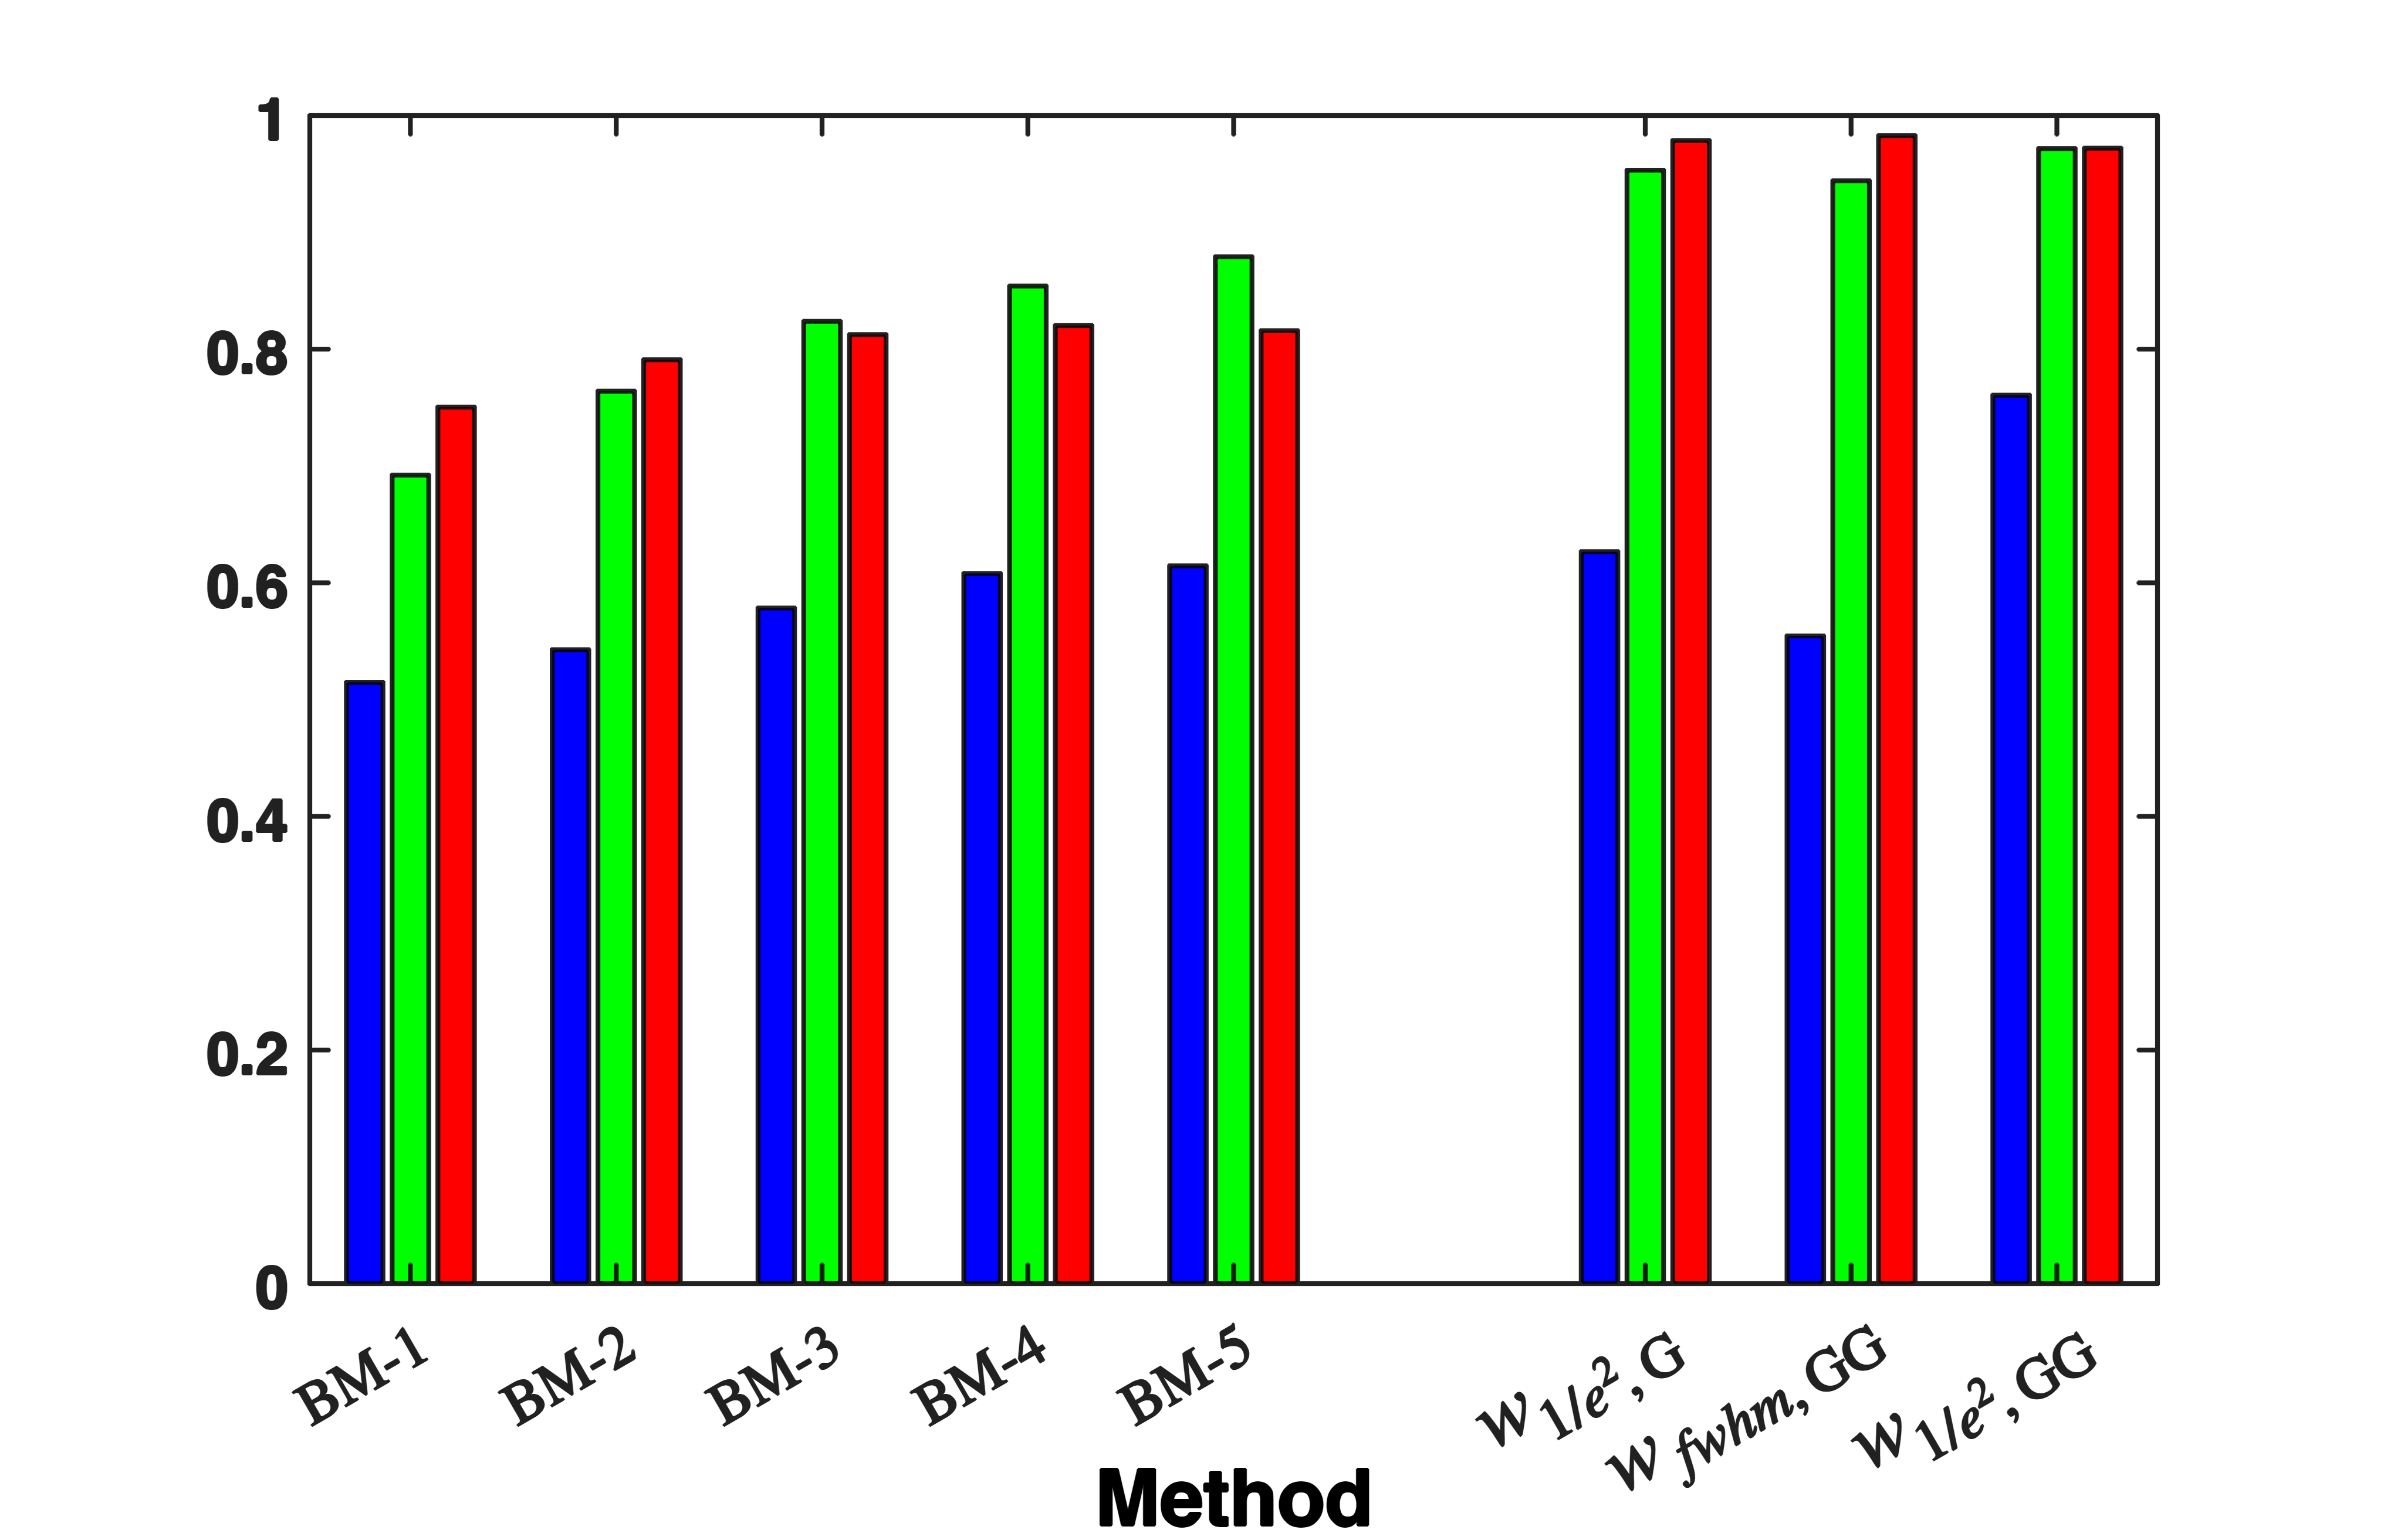
\includegraphics[width=\linewidth,trim=148 0 361 145,clip]{figures/cov_r2_d.png}\end{subfigure}
\caption{Summary of linearity and precision across all diameter measurement methods. (a, b) Coefficient of variation (CoV), a measure of precision, and (c, d) coefficient of determination ($R^2$), a measure of linearity and hence of how reliably a measurement can be corrected, for MIP (a, c) and MeIP (b, d), respectively. Bars are grouped by method (BM-1 through BM-5, $w_{1/e^2,\,\mathrm{G}}$, $w_{fwhm,\,\mathrm{GG}}$, $w_{1/e^2,\,\mathrm{GG}}$) and colour-coded by contrast conditions.}
\label{fig:cov_r2}
\end{figure}

\subsection{Functional flicker stimulation}
\label{subsec:flicker}  
To evaluate how each method performed under a controlled induction of diameter change, flicker stimulation was used to evoke vasodilation while the same vessels were tracked over time. For the binary-mask-based measurements, BM-5 applied to the MeIP was used, as this combination gave the lowest CoV (0.09) and the joint-highest $R^2$ (0.82) post-contrast. Its slope was further from unity ($m = 0.86$), but that bias is systematic and correctable by calibration. The model-based measurements showed significant diameter increases in four of five vessels ($p < 0.01$), evident in the time series and confirmed by the mean diameters before and after stimulation (Figs.~\ref{fig:flicker}a,b,d,e and Table~\ref{tab:flicker}). The binary-mask-based time series showed a mixed trend, but the mean diameters revealed significant decreases in four of five vessels (Figs.~\ref{fig:flicker}c,f). Of the three methods, the GG model agreed most closely with the ground truth (Figs.~\ref{fig:flicker}d--f).

To assess whether angiogram intensity itself biases the diameter measurements, we examined the intensity time series alongside the diameter time series and looked at intensity correlations. The binary-mask-based method showed uniformly positive per-vessel correlations, with an overall correlation of $\rho = 0.526$ (Fig.~\ref{fig:scatter_intensity}c) measured as the average of the individual correlations. The Gaussian and GG models yielded overall correlations of $\rho = -0.101$ and $\rho = -0.098$, respectively (Fig.~\ref{fig:scatter_intensity}a,b). The angiogram intensity time series (Fig.~\ref{fig:flicker}g) showed a visible decline in angiogram intensity throughout the duration of the DyC-OCT scan across all five vessels. The mean intensity comparison pre- and post-stimulation (Fig.~\ref{fig:flicker}h) confirmed that the decrease was significant for all vessels, ranging from $-13.6\%$ to $-19.8\%$ (Table~\ref{tab:flicker}). 

\begin{figure}[htbp]
\centering
\setlength{\abovecaptionskip}{2pt}\setlength{\belowcaptionskip}{2pt}
\captionsetup[subfigure]{position=top,font=bf,skip=2pt}
\begin{subfigure}{0.32\linewidth}\centering\captionsetup{margin={4.90mm,0mm}}\caption{Gaussian model}\label{fig:flicker_a}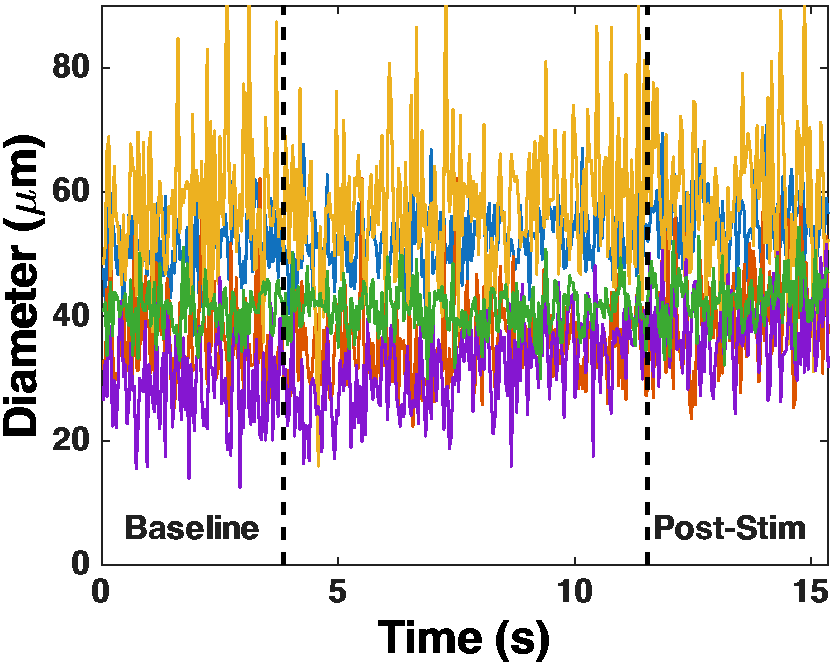
\includegraphics[width=\linewidth]{figures/flicker_a.pdf}\end{subfigure}\hfill%
\begin{subfigure}{0.32\linewidth}\centering\captionsetup{margin={4.90mm,0mm}}\caption{GG model}\label{fig:flicker_b}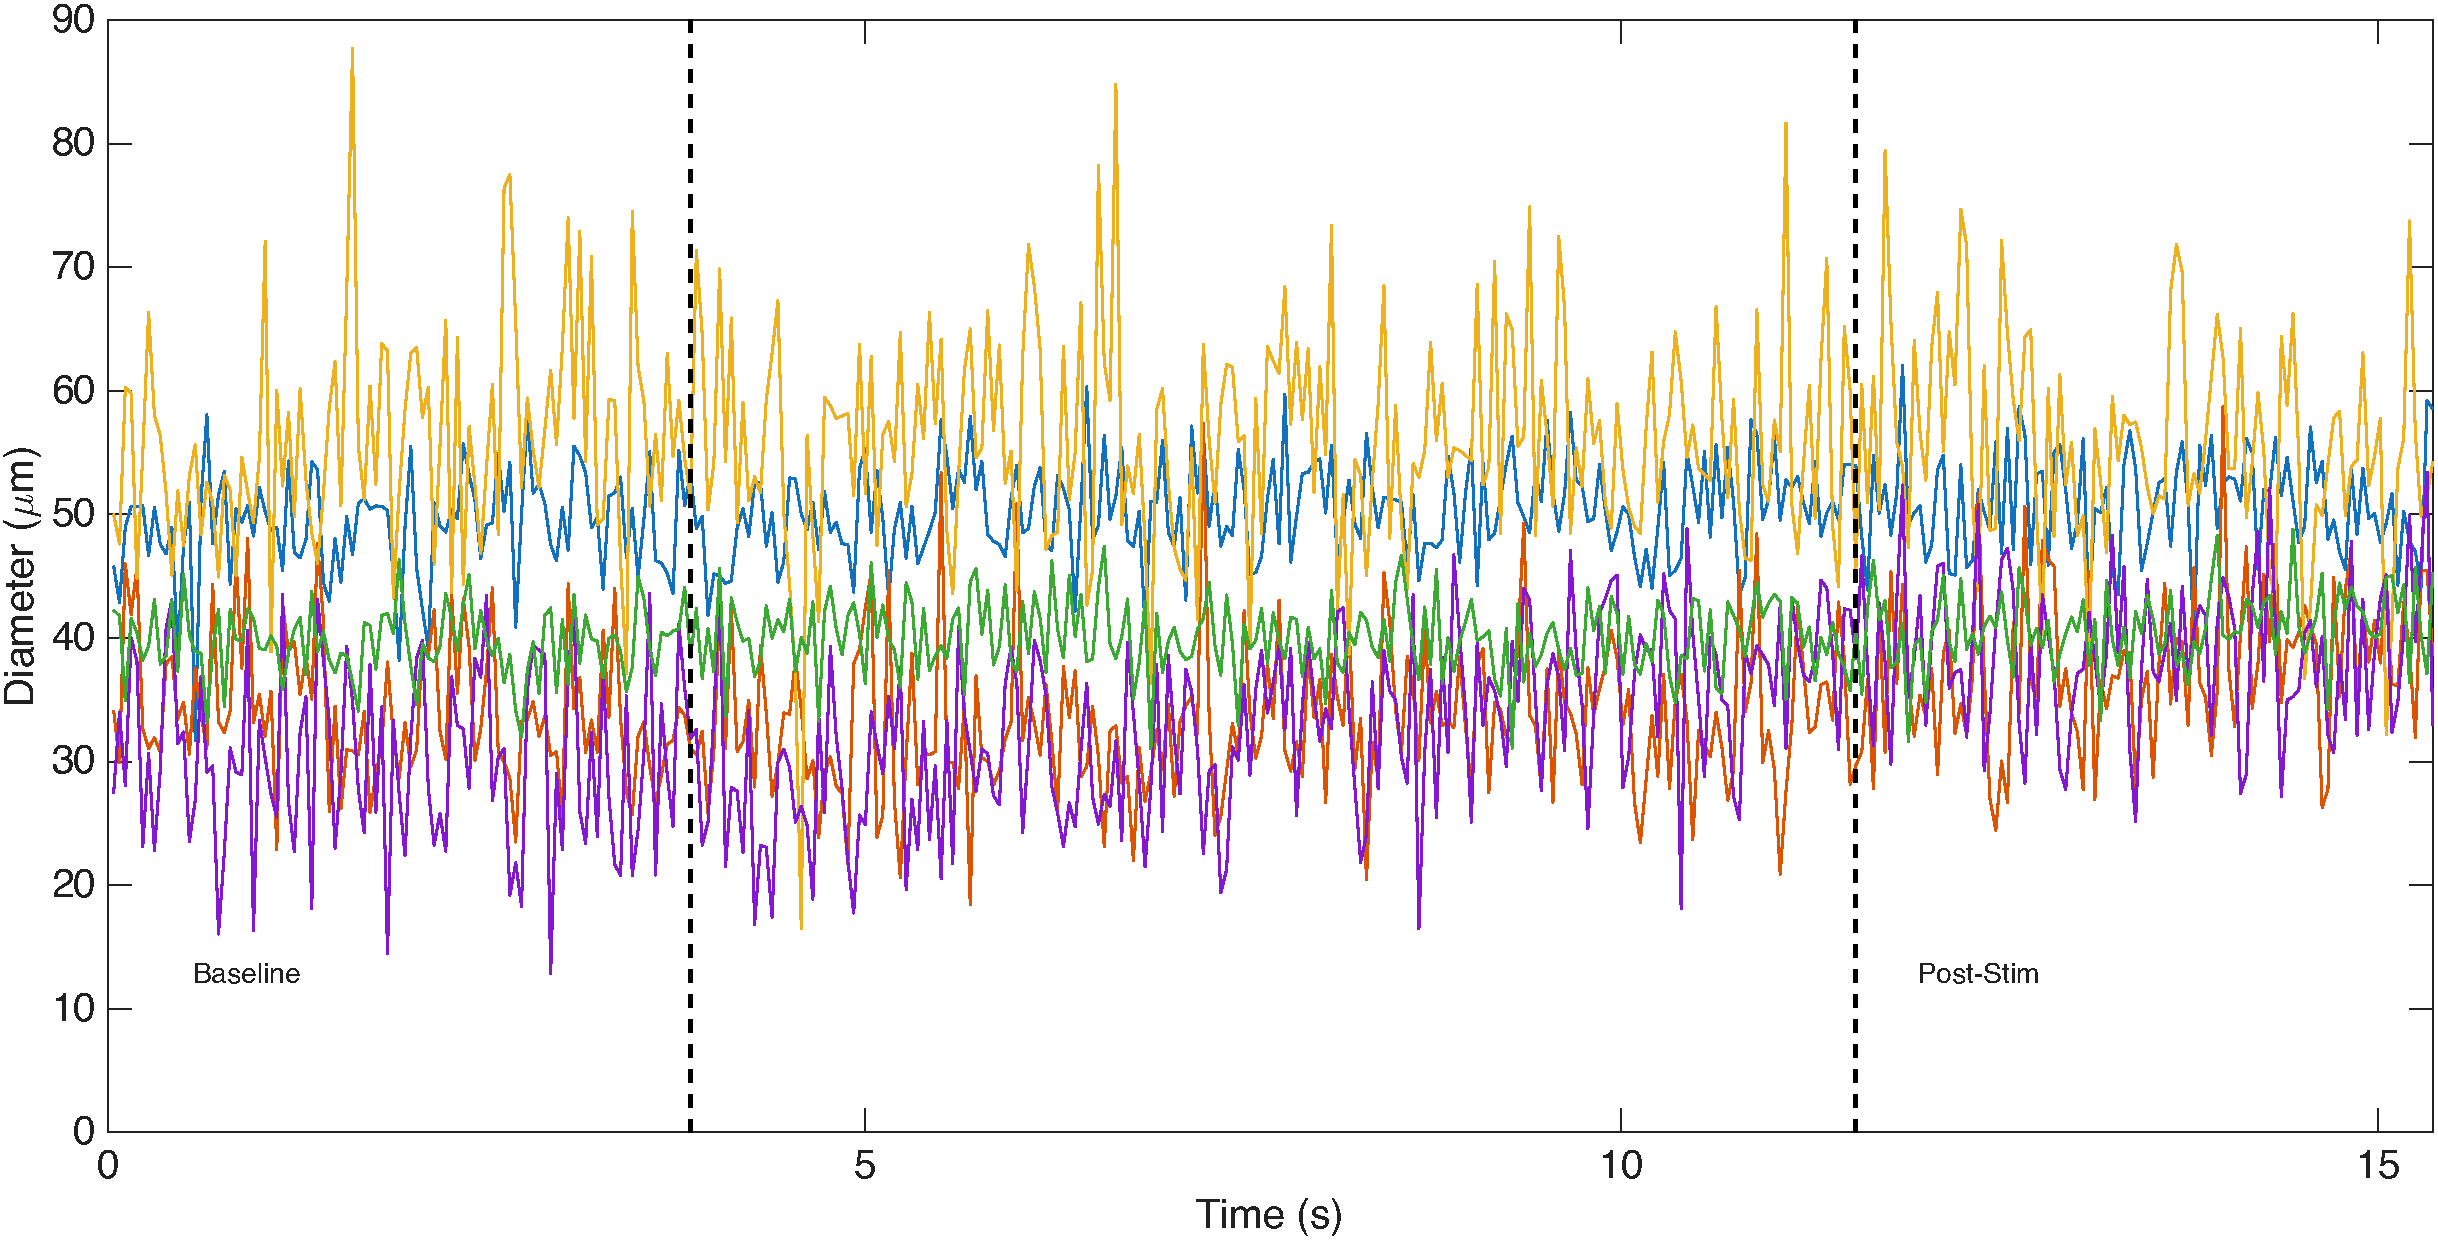
\includegraphics[width=\linewidth]{figures/flicker_b.pdf}\end{subfigure}\hfill%
\begin{subfigure}{0.32\linewidth}\centering\captionsetup{margin={4.90mm,0mm}}\caption{Binarised angiogram}\label{fig:flicker_c}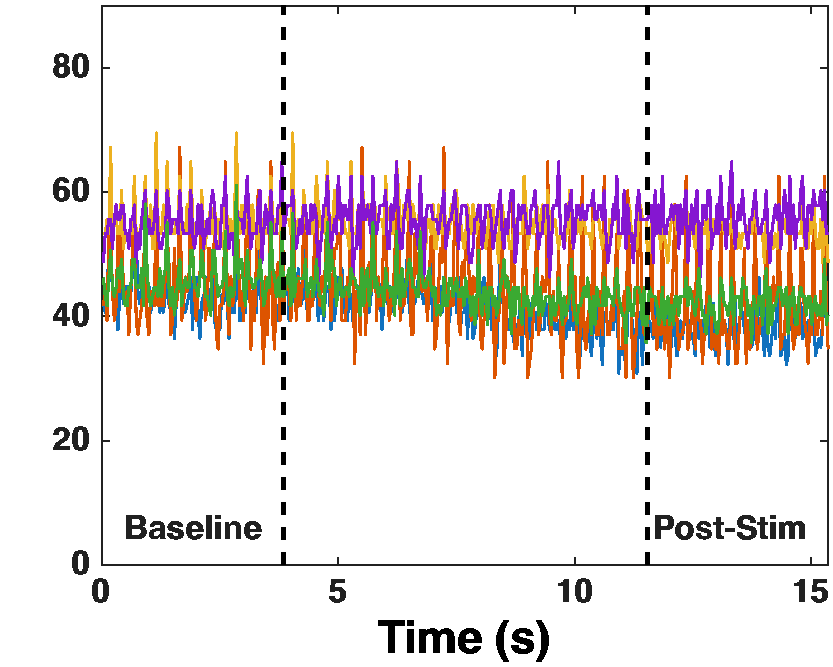
\includegraphics[width=\linewidth]{figures/flicker_c.pdf}\end{subfigure}\\
\begin{subfigure}{0.32\linewidth}\centering\captionsetup{margin={4.90mm,0mm}}\caption{Gaussian model}\label{fig:flicker_d}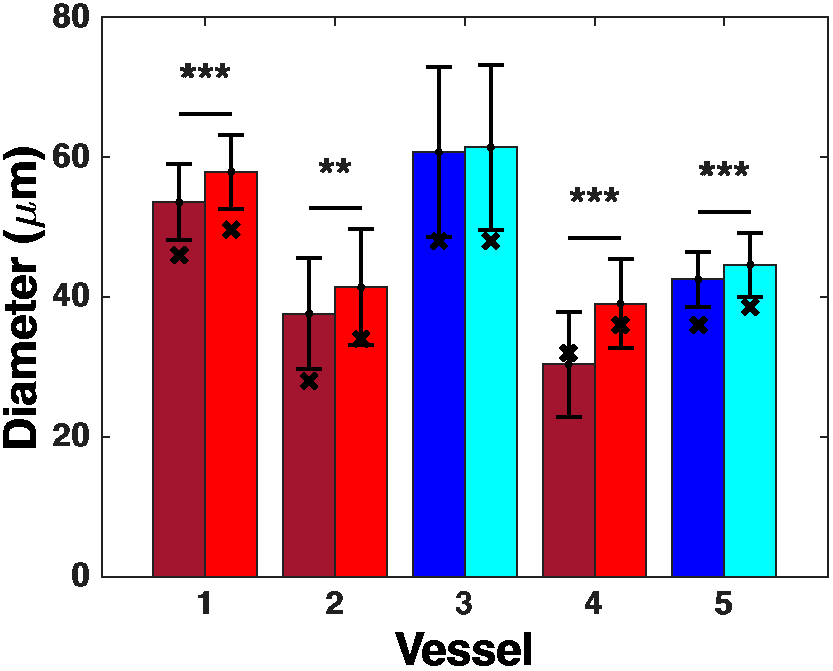
\includegraphics[width=\linewidth]{figures/flicker_d.pdf}\end{subfigure}\hfill%
\begin{subfigure}{0.32\linewidth}\centering\captionsetup{margin={4.90mm,0mm}}\caption{GG model}\label{fig:flicker_e}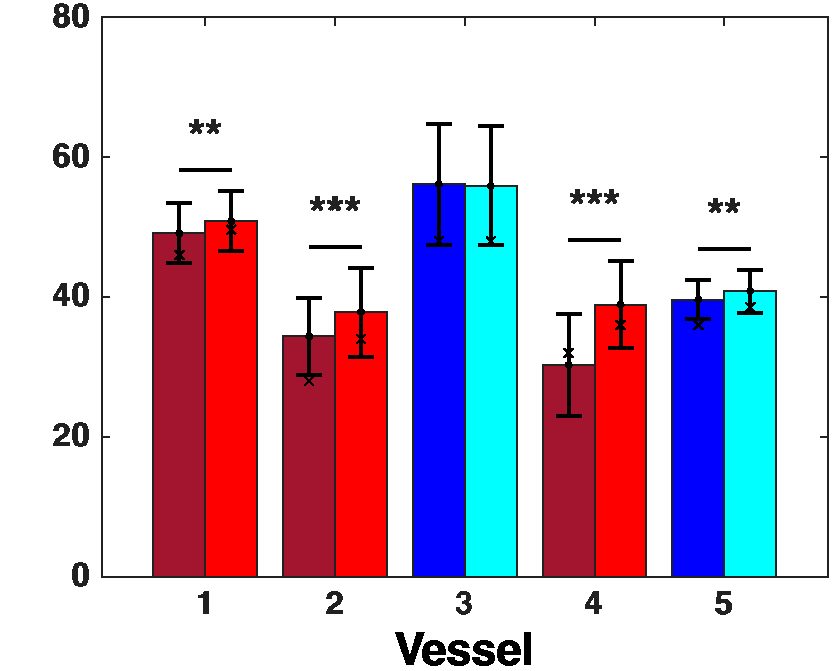
\includegraphics[width=\linewidth]{figures/flicker_e.pdf}\end{subfigure}\hfill%
\begin{subfigure}{0.32\linewidth}\centering\captionsetup{margin={4.90mm,0mm}}\caption{Binarised angiogram}\label{fig:flicker_f}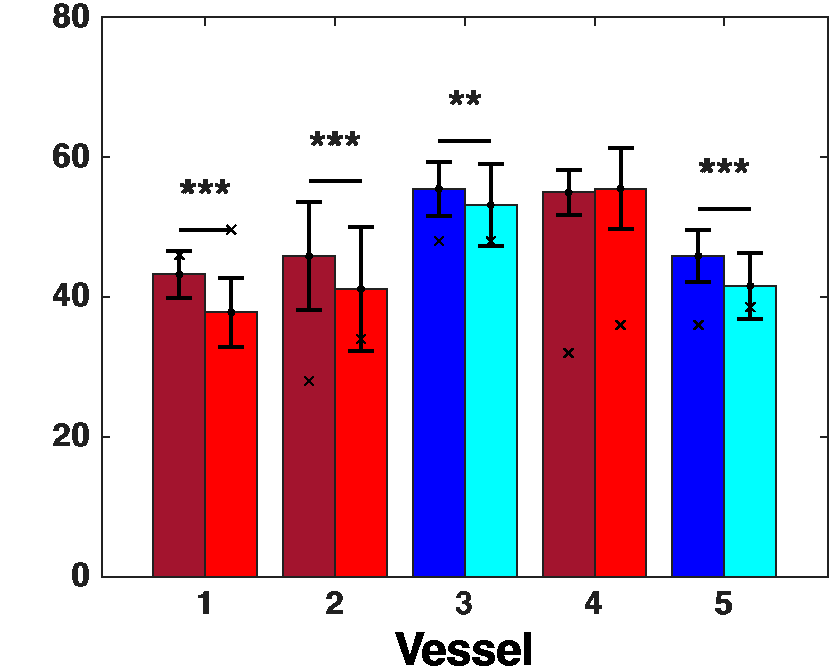
\includegraphics[width=\linewidth]{figures/flicker_f.pdf}\end{subfigure}\\
\begin{subfigure}{0.32\linewidth}\centering\captionsetup{margin={5.40mm,0mm}}\caption{Angiogram intensity}\label{fig:flicker_g}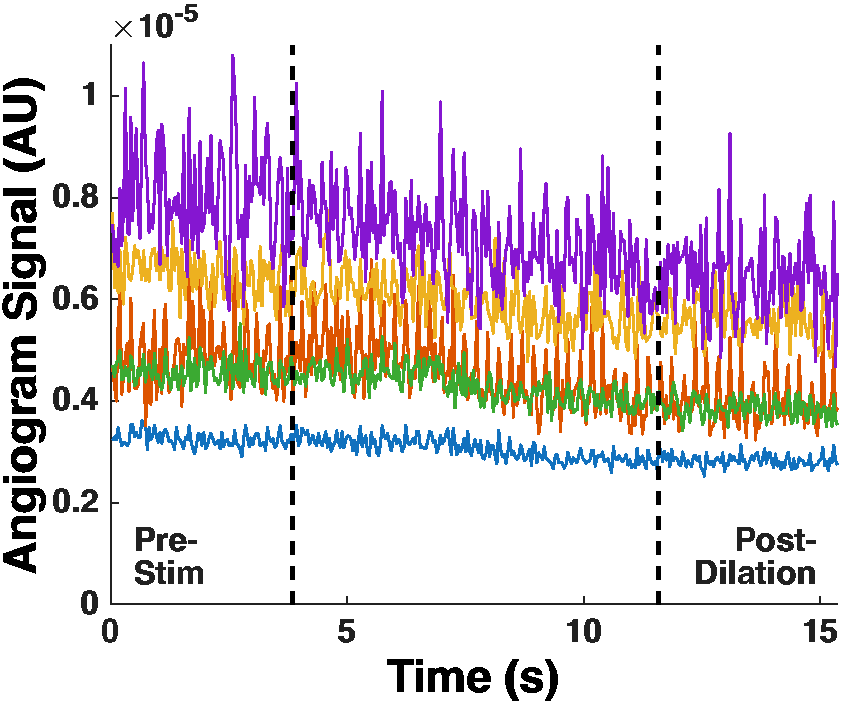
\includegraphics[width=\linewidth]{figures/flicker_g.pdf}\end{subfigure}\hfill%
\begin{subfigure}{0.32\linewidth}\centering\captionsetup{margin={2.70mm,-2.70mm}}\caption{Mean angiogram intensity}\label{fig:flicker_h}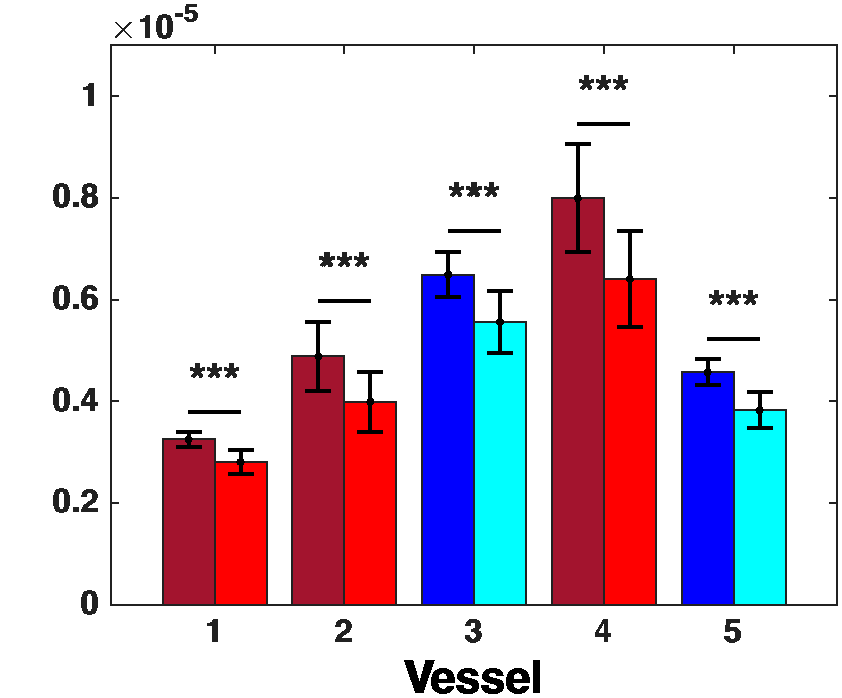
\includegraphics[width=\linewidth]{figures/flicker_h.pdf}\end{subfigure}\hfill%
\begin{subfigure}[t]{0.32\linewidth}\centering\raisebox{14pt}{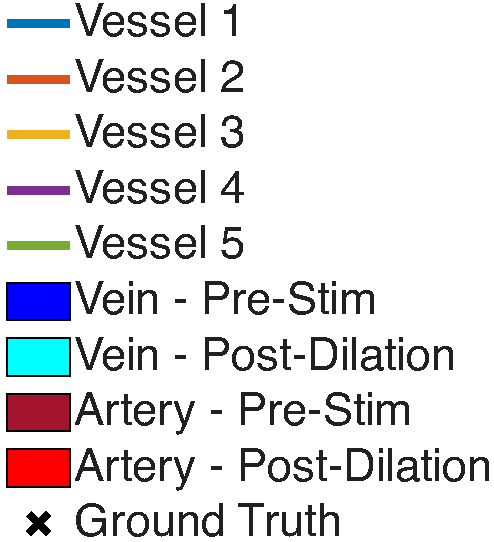
\includegraphics[width=0.6\linewidth]{figures/flicker_legend.pdf}}\end{subfigure}
\caption{Functional flicker stimulation results.~(a--c) Vessel diameter time series pre- and post-stimulation across five vessels.~(d--f) Mean diameter per vessel before (dark bars) and after (light bars) stimulation for each method. Veins are shown in blue/cyan and arteries in dark/light red.~(g) Angiogram intensity time series. (h) Mean angiogram intensity per vessel pre- and post-stimulation. All measurements used MeIP. Crosses $\boldsymbol{(\times)}$ indicate the ground truth diameter for each vessel. Significance levels: $^{*}p < 0.05$, $^{**}p < 0.01$, $^{***}p < 0.001$.}
\label{fig:flicker}
\end{figure}

\begin{figure}[htbp]
\centering
\setlength{\abovecaptionskip}{4pt}\setlength{\belowcaptionskip}{2pt}
\captionsetup[subfigure]{position=top,font=bf,skip=2pt}
\begin{subfigure}{0.32\linewidth}\centering\captionsetup{margin={4.55mm,0mm}}\caption{Gaussian model}\label{fig:scatter_intensity_a}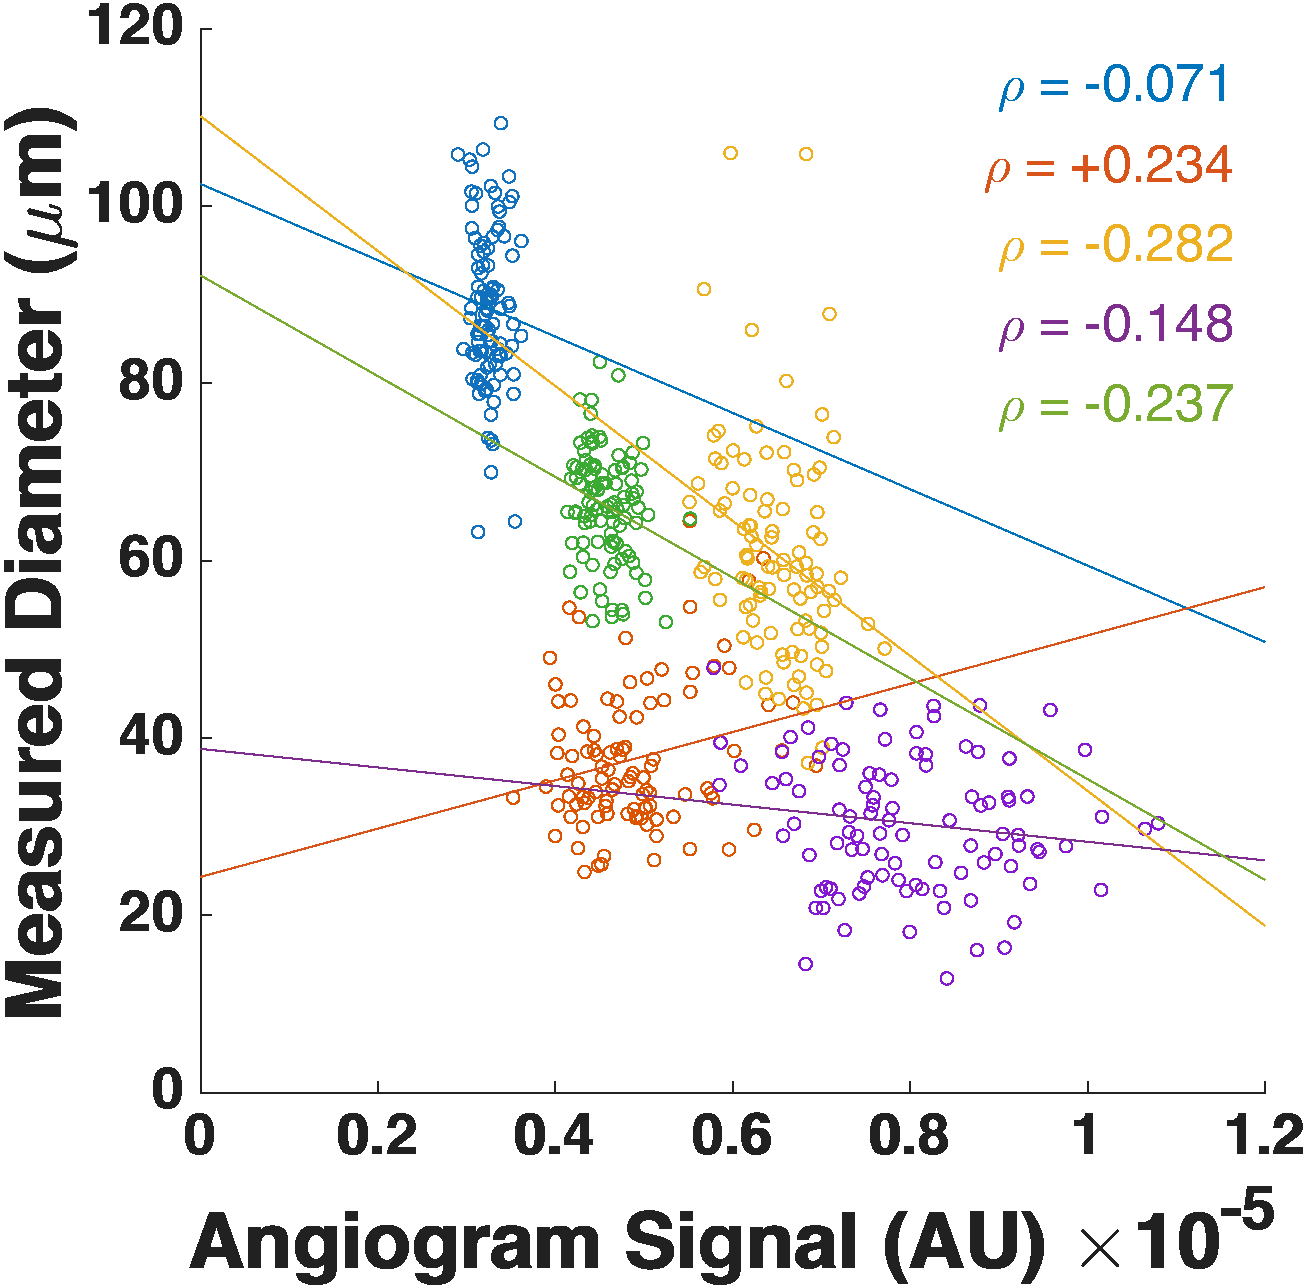
\includegraphics[width=\linewidth]{figures/scatter_intensity_a.pdf}\end{subfigure}\hfill%
\begin{subfigure}{0.32\linewidth}\centering\captionsetup{margin={4.55mm,0mm}}\caption{GG model}\label{fig:scatter_intensity_b}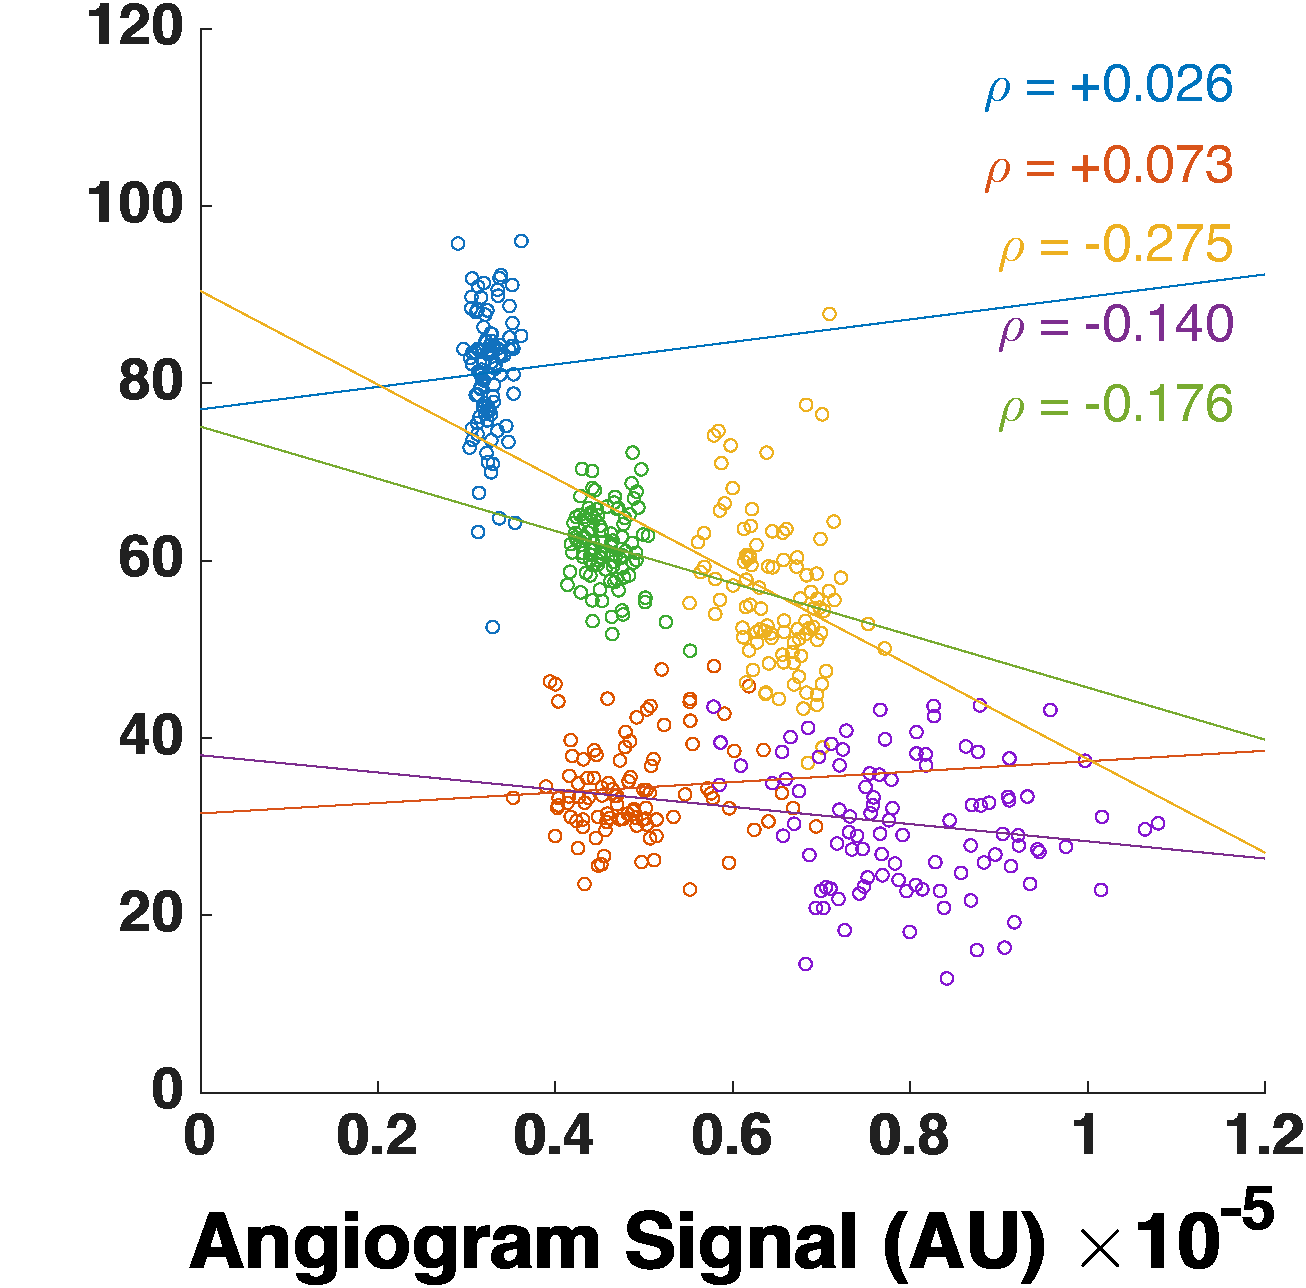
\includegraphics[width=\linewidth]{figures/scatter_intensity_b.pdf}\end{subfigure}\hfill%
\begin{subfigure}{0.32\linewidth}\centering\captionsetup{margin={4.55mm,0mm}}\caption{binary-mask-based}\label{fig:scatter_intensity_c}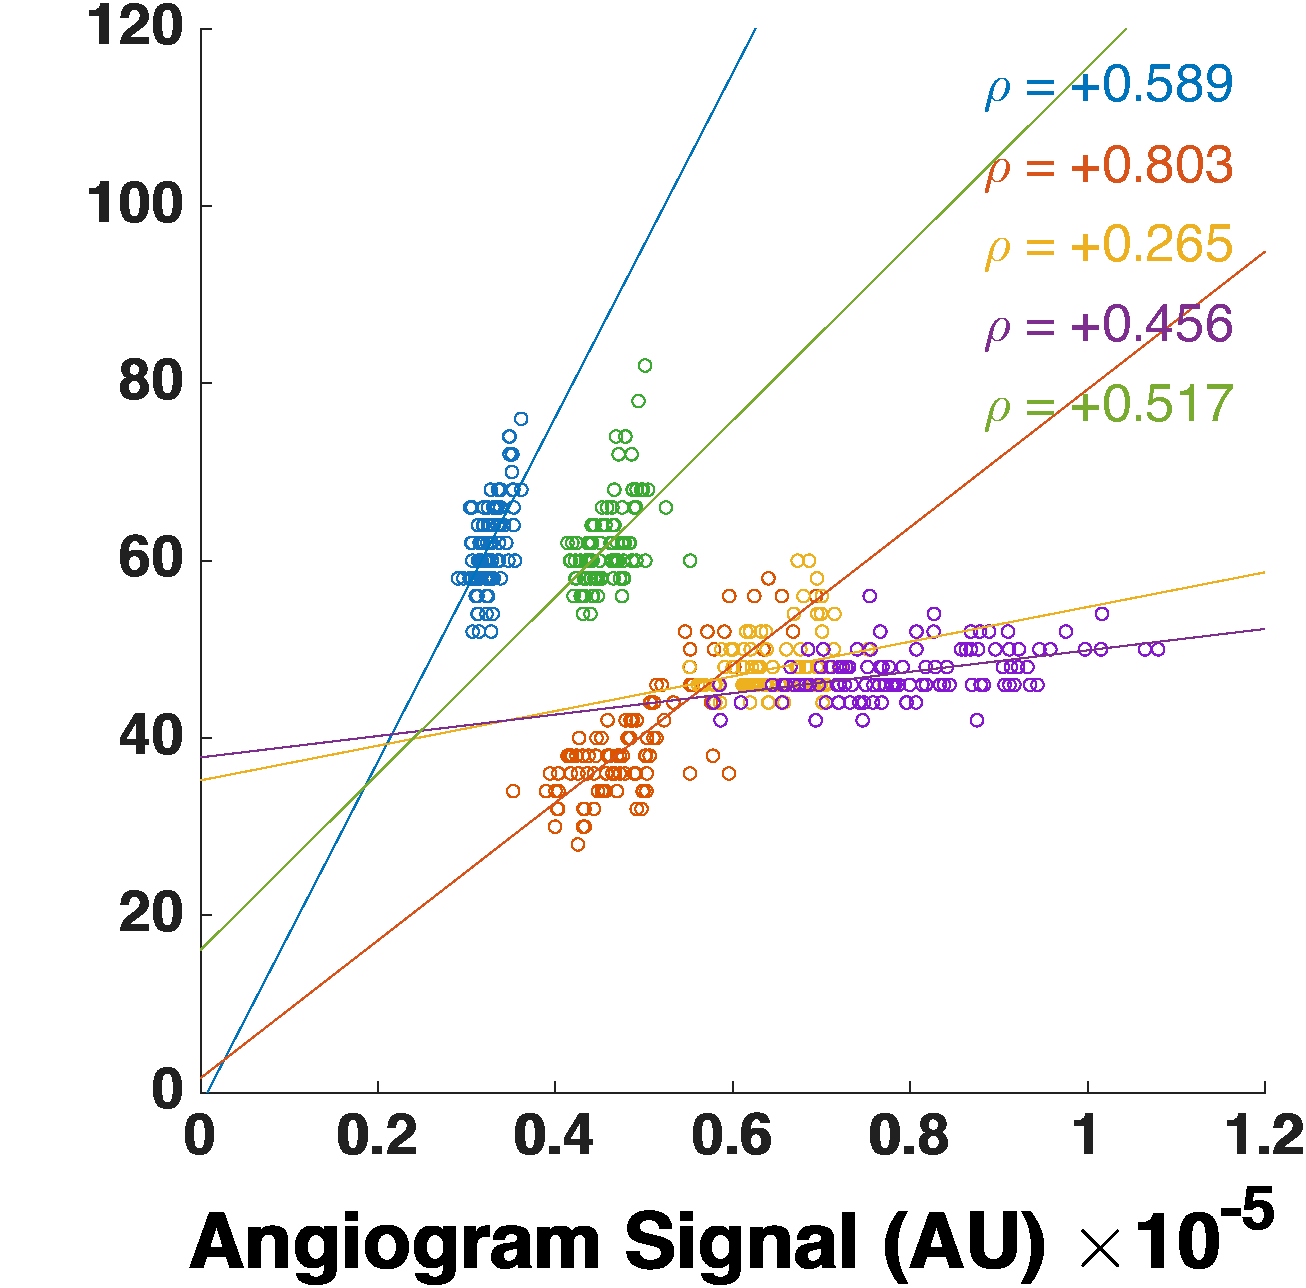
\includegraphics[width=\linewidth]{figures/scatter_intensity_c.pdf}\end{subfigure}
\caption{Measured vessel diameter as a function of angiogram signal intensity during functional flicker stimulation for (a) Gaussian model, (b) generalised Gaussian model, and (c) binary-mask-based method. Each colour represents one of five vessels. $\rho$ denotes the Pearson correlation coefficient.}
\label{fig:scatter_intensity}
\end{figure}

\begin{table}[htb]
\caption{Flicker stimulation results. $\Delta d$: diameter change (\%); $\rho$: Correlation between diameter and angiogram intensity; $\Delta I$: intensity change (\%). Statistically significant values are bold. Significance levels: $^{*}p < 0.05$, $^{**}p < 0.01$, $^{***}p < 0.001$.}
\label{tab:flicker}
\centering
\setlength{\abovecaptionskip}{2pt}\setlength{\belowcaptionskip}{2pt}
\footnotesize
\resizebox{\textwidth}{!}{%
\begin{tabular}{l | c c | c c | c c | c | c}
\hline
 & \multicolumn{2}{c|}{\textbf{Gaussian}} & \multicolumn{2}{c|}{\textbf{GG}} & \multicolumn{2}{c|}{\textbf{Binarised}} & \textbf{Intensity} & \textbf{Ground Truth} \\
 & $\Delta d$ (\%) & $\rho$ & $\Delta d$ (\%) & $\rho$ & $\Delta d$ (\%) & $\rho$ & $\Delta I$ (\%) & $\Delta d$ (\%) \\
\hline
Vessel 1 (Artery) & $\mathbf{+8.2}^{***}$ & $-0.07$ & $\mathbf{+3.5}^{**}$ & $0.03$ & $\mathbf{-12.5}^{***}$ & $\mathbf{0.59}^{***}$ & $\mathbf{-13.6}^{***}$ & $+7.9$ \\
Vessel 2 (Artery) & $\mathbf{+9.9}^{**}$ & $\mathbf{0.23}^{*}$ & $\mathbf{+10.1}^{***}$ & $0.07$ & $\mathbf{-10.2}^{***}$ & $\mathbf{0.80}^{***}$ & $\mathbf{-18.2}^{***}$ & $+21.4$ \\
Vessel 3 (Vein) & $+1.2$ & $\mathbf{-0.28}^{**}$ & $-0.4$ & $\mathbf{-0.28}^{**}$ & $\mathbf{-4.1}^{**}$ & $\mathbf{0.27}^{**}$ & $\mathbf{-14.3}^{***}$ & $+0.0$ \\
Vessel 4 (Artery) & $\mathbf{+28.5}^{***}$ & $-0.15$ & $\mathbf{+28.4}^{***}$ & $-0.14$ & $+1.0$ & $\mathbf{0.46}^{***}$ & $\mathbf{-19.8}^{***}$ & $+12.5$ \\
Vessel 5 (Vein) & $\mathbf{+4.9}^{***}$ & $\mathbf{-0.24}^{*}$ & $\mathbf{+3.1}^{**}$ & $-0.18$ & $\mathbf{-9.3}^{***}$ & $\mathbf{0.52}^{***}$ & $\mathbf{-16.3}^{***}$ & $+7.1$ \\
\hline
Overall $\rho$ & & $-0.101$ & & $-0.098$ & & $0.526$ & & \\
Overall arterial change & $+15.5$ & & $+14.0$ & & $-7.2$ & & $-17.2$ & $+13.9$ \\
Overall venous change & $+3.1$ & & $+1.4$ & & $-6.7$ & & $-15.3$ & $+3.6$ \\
\hline
\end{tabular}%
}
\end{table}

\section{Discussion}
\subsection{Model-based vs. binary-mask-based diameter measurement}
\label{subsec:model_vs_binary}
The model-based and binary-mask-based diameter methods define vessel boundary in fundamentally different ways. Binarisation of the en face maps discards the spatial intensity distribution for a simple binarisation and reduces each pixel to a binary decision. The measured diameter directly depends on the chosen threshold value and on angiogram intensity, both of which may vary across imaging sessions, contrast conditions, and even between vessels within the same scan. Model-based methods fit a parametric model function to the maximum or mean intensity profiles and calculate the diameter from the fitted parameters. As the fit captures the shape of the profile rather than the absolute intensity, it is inherently less sensitive to changes in angiogram signal, and the level at which the diameter is defined is intensity-independent rather than set by the absolute intensity of the image.

A practical consequence of this difference is how correctable each method is. Although both methods take input parameters to determine the measured diameter, the model-based diameter is determined relative to the fitted profile and is therefore intensity-independent. In contrast, the binarisation slope shifts with vessel intensity, so any calibration must also account for the intensity threshold used. Systematic diameter underestimation can be corrected by a fixed proportion using the slope, provided the relationship with the ground truth is strongly linear, but such a rescaling removes only the systematic proportional bias and leaves the scatter about the regression unchanged. Linearity, rather than slope alone, therefore determines how reliably a method can be corrected. Post-contrast every model-based metric reached $R^2 \geq 0.92$, whereas binary-mask-based MIP, which is the most commonly used~\cite{sampsonTowardsStandardizingRetinal2022,untrachtTowardsStandardisingRetinal2024}, ranged from 0.48 at BM-5 to 0.81 at BM-1. The improved linearity of the model-based metrics makes them more predictable/systematic even pre-contrast, where $w_{1/e^2,\mathrm{GG}}$ retained $R^2 = 0.81$ against 0.62 for the best binary-mask-based method.

This difference explains the trends observed in Fig.~\ref{fig:cov_r2} and Table~\ref{tab:accuracy_linearity}. Post-contrast, every model-based metric was more linear than every binary-mask-based method, and the GG $1/e^2$ metric reached near-unity slopes at peak and post-contrast without an intensity threshold parameter to tune, whereas for the binary-mask-based methods linearity was overall lower and depended on threshold using the global thresholding described here. Because the peak angiogram intensity varies between vessels, a fixed threshold removes a different fraction of the cross-section from each one. The measured diameters therefore vary from the ground truth by different amounts, which weakens the linearity. Pre-contrast, the hourglass artefact caused by RBC orientation within vessel lumen suppresses edge signals~\cite{cimallaShearFlowinducedOptical2011,bernucciInvestigationArtifactsRetinal2018}, causing all methods to underestimate diameter. However, model-based methods still retained more of that linearity, producing systematic, predictable underestimation. Binary-mask-based methods, on the other hand, showed weaker linearity in most conditions, potentially because the suppressed edge signals did not consistently exceed the binarisation threshold, and because different vessels have different intensity.

The same mechanism accounts for how each method responded to the change in angiogram intensity from peak to post-contrast. Angiogram intensity is highest as the bolus arrives and then settles to a lower steady state (Fig.~\ref{fig:dycoct}f), so a fixed threshold encloses a smaller fraction of each cross-section post-contrast than at peak, an effect visible in the binarised cross-sections over time (Fig.~\ref{fig:dycoct}d,e). Model-based metrics were largely insensitive to this, changing by at most 0.04 in slope and 0.04 in $R^2$ between the two conditions. Binary-mask-based measurements from MIP degraded progressively with threshold, the slope falling by 0.04 at BM-1 but 0.11 at BM-5, and $R^2$ by 0.07 and 0.30 respectively, while MeIP remained comparatively stable (slope change 0.02--0.03 at every threshold). Model-based methods therefore showed comparable agreement with the ground truth at both peak and post-contrast, whereas the agreement of binary-mask-based method depended on the combination of threshold and contrast condition.

In this study we observed that the generalised Gaussian (GG) model outperformed the standard Gaussian, because the intensity profiles of the vessels were usually not purely Gaussian (Fig.~\ref{fig:gg_model}b). The standard Gaussian cannot capture relatively flat-topped angiogram intensity profiles and tends to fit a narrower curve, whereas the GG model accommodates through the shape parameter $\beta$ (Fig.~\ref{fig:gg_model}b). The flat-topped shapes arise because the measured profile is effectively the vessel's reflectivity profile convolved with the system point spread function. Because the GG reduces to a standard Gaussian when $\beta = 2$ and departs from it only when the data support a flatter profile, a correctly applied GG fit should perform at least as well as the Gaussian, at the cost of additional computation.

Among the width metrics, $w_{fwhm,\,\mathrm{GG}}$ consistently showed the greatest underestimation, although its linearity remained high post-contrast ($R^2$ = 0.96 for MIP and 0.98 for MeIP), indicating that the underestimation is systematic and therefore correctable. Near the half-maximum the profile shape changes rapidly and varies between vessels, from Gaussian to flat-topped, so the width measured at that level is more variable. The $1/e^2$ width captures more of the transition region and so may have provided a more accurate measurement of the vessel diameter. These results suggest that the generalised Gaussian $1/e^2$ metric was the most reliable of the model-based options, showing both the closest agreement with the ground truth, strongest linearity, and highest precision.

\subsection{Maximum vs. mean intensity projection}
\label{subsec:max_vs_mean}
Across nearly all methods and conditions, MeIP outperformed MIP in both accuracy and precision (Table~\ref{tab:accuracy_linearity}). Linearity was the exception. Pre-contrast MIP produced higher $R^2$ than MeIP for all model-based metrics, and MIP also produced higher $R^2$ at the two lowest binarisation thresholds, with MeIP outperforming MIP only post-contrast.  This finding is noteworthy because MIP has been shown to produce higher signal-to-noise ratio (SNR) and contrast in en face OCTA images~\cite{hormelMaximumValueProjection2018}, and is the default in many commercial OCTA systems and analysis pipelines~\cite{sampsonTowardsStandardizingRetinal2022,untrachtTowardsStandardisingRetinal2024}. However, we observed that higher SNR did not necessarily translate to more accurate diameter measurements. The MIP selects the single highest intensity value along each A-scan within the vessel ROI, which makes it inherently sensitive to outliers. MeIP averages all intensity values along each A-scan, which smooths out intensity fluctuations and provides a consistent profile. This averaging could be beneficial for vessel diameter measurement, as the goal is to capture the typical vessel boundary rather than extreme signal events. This trade-off may also explain why linearity behaved differently before and after contrast. Pre-contrast the vessel signal is weakest, and edge suppression by the RBC orientation artefact leaves little margin above the background, so the higher contrast of the MIP helps keep the profile distinguishable across vessels of different size. Once the lumen is filled with contrast agent, signal is no longer limiting and the outlier sensitivity of a maximum statistic may contribute more strongly to the measurement error, so the averaging of the MeIP yields the tighter relationship with the ground truth. Consistent with this, MeIP produced higher $R^2$ than MIP for all three model-based metrics post-contrast, whereas at peak contrast the two projections remained comparable, with MIP higher for two of the three model-based metrics.

The difference between MIP and MeIP was especially apparent in the binary-mask-based results (Table~\ref{tab:accuracy_linearity}). For MeIP, the slope declined more gradually and remained at 0.86 even at BM-5 post-contrast. Whereas for MIP, the slope decreased steeply with increasing threshold, dropping from 0.92 at BM-1 to 0.54 at BM-5 post-contrast. These findings suggest that MeIP produces a more uniform intensity distribution across the vessel profile, making the binarisation result less sensitive to the exact threshold value. The CoV data (Table~\ref{tab:accuracy_linearity}) reinforced this as the MIP-based binary mask CoV increased substantially with threshold, whereas the MeIP-based CoV remained relatively stable. This behaviour follows from how each projection responds to variance in the angiogram signal. Because the MIP keeps only the brightest pixel along each A-scan, it tracks whichever value happens to be largest, so the projected profile fluctuates from one time sample to the next. A threshold applied to a fluctuating profile returns a fluctuating width. How much the width fluctuates depends on where the threshold cuts the profile. A low threshold cuts the steep flanks of the profile, where a change in intensity moves the measured edge only slightly. A high threshold cuts near the flat top, where the same change moves it much further. The CoV therefore grows as the threshold is raised. MeIP averages along each A-scan instead, which suppresses the fluctuation and gives a broader, smoother profile, so its CoV changes little as the threshold increases. For model-based methods, MeIP also showed better performance. The $w_{1/e^2,\,\mathrm{G}}$ using MIP slightly overestimated vessel diameter post-contrast with $m = 1.12$, while MeIP reduced this to $m = 1.04$, a much closer agreement with the ground truth. These results suggest that while MIP may be preferred for visualisation purposes where contrast and SNR are important~\cite{hormelMaximumValueProjection2018}, MeIP should be the preferred projection method for quantitative diameter measurements using the methods evaluated here.

\subsection{Influence of angiogram intensity on diameter measurements}
\label{subsec:influence_of_intensity}
The functional flicker stimulation experiment provided a direct demonstration of how changes in angiogram signal intensity can affect diameter measurements based on the method used. During the DyC-OCT acquisition, the angiogram intensity declined significantly across all five vessels (Fig.~\ref{fig:flicker}g,h), with decreases ranging from $-13.6\%$ to $-19.8\%$ (Table~\ref{tab:flicker}). The cause of this decline was not established with certainty, although inspection of the volumetric data ruled out the most important confounds. There was no obvious out-of-plane motion or breathing artefact, and the image quality was consistent throughout the scan. We suspect a combination of rapid corneal drying and/or cataract formation over the course of the scan could have caused the decline in intensity. More importantly, the cause of the decline does not affect our observation that the intensity decline was associated with changes in the binary-mask-based measurements, while the model-based measurements were less affected. 

The model-based methods correctly detected the expected vasodilation, with the Gaussian model showing significant diameter increases in four of five vessels ($+15.5\%$ overall in the arteries against $+3.1\%$ in the veins) and the GG model showing significant increases in four of five vessels ($+14.0\%$ and $+1.4\%$ respectively; Table~\ref{tab:flicker}). The binary-mask-based method, however, reported significant diameter decreases in four of five vessels, suggesting vasoconstriction which is a paradoxical result. The reason behind this behaviour could be understood by observing how each method responds to declining signal intensity (Fig.~\ref{fig:scatter_intensity}). For the binary-mask-based method, the threshold is fixed and diameter is determined by the number of pixels that exceed this threshold. When the overall angiogram intensity drops, fewer pixels at the vessel edges exceed the threshold, and the vessel appears to shrink even if the physical vessel diameter has increased. This is confirmed by the strong positive correlation between measured diameter and angiogram intensity for the binary-mask-based method ($\rho = 0.526$, $p < 0.0005$). In contrast, the model-based methods showed weak overall correlations with intensity ($\rho = -0.101$ for Gaussian, $\rho = -0.098$ for GG), indicating that the fitted diameter was effectively independent of the signal intensity. Among the methods, the GG model also produced the lowest standard deviations across the five vessels in the flicker experiment (Fig.~\ref{fig:flicker}d--f), consistent with its low CoV post-contrast (Table~\ref{tab:accuracy_linearity}), indicating that it is the most repeatable of the metrics tested. It also showed the closest agreement with ground truth. Together these results demonstrated that the model-based diameter calculation provided more accurate and repeatable measurements, and recovered physiologically meaningful vascular responses that binary-mask-based methods misidentified.

These findings have important implications for longitudinal studies and any experiment where angiogram intensity may vary between or within imaging sessions. In longitudinal mouse eye imaging, the angiogram signal can vary between and within sessions as anaesthesia alters retinal perfusion and ocular physiology~\cite{wormRetinalOCTParameters2026,fengHighresolutionStructuralFunctional2023}, with additional factors such as cataract formation, and corneal drying if tear drops are not applied, further reducing OCT intensity over time~\cite{steinEffectCornealDrying2006,mclellanOpticalCoherenceTomography2012}. If a binary-mask-based method is used under such conditions, observed changes in vessel diameter may reflect intensity fluctuations rather than true vascular changes. In contrast, model-based methods may be less sensitive to these intensity variations, as they characterise the shape of the intensity profile rather than relying primarily on absolute intensity values to define vessel boundaries.

\subsection{Threshold selection}
\label{subsec:threshold_selection}
The results presented here were based on a basic, global threshold for the binarisation of the angiogram data. There are numerous other approaches for binarising the angiogram, which will most likely each behave differently \cite{mehtaImpactBinarizationThresholding2019,rabioloComparisonMethodsQuantify2018,borrelliOPTICALCOHERENCETOMOGRAPHY2021,freedmanImpactImageProcessing2022,arrigoImpactDifferentThresholds2021}. For example, angiogram signals can be enhanced with vesselness filters~\cite{frangiMultiscaleVesselEnhancement1998} and dynamic thresholds can be used to binarise images with varying SNR. When applying a vesselness filter, it is possible to enhance the shape of the angiogram and omit noise, but it is also possible for such enhancement to overcompensate the signal, leading to larger than expected vessel appearance. Measurements obtained with different enhancement filters have been shown to differ substantially and are not interchangeable~\cite{hongEffectVesselEnhancement2020}. Dynamic thresholding can also yield a more uniform angiogram appearance, but similarly risks over- or under-compensating vessels. The threshold chosen is known to alter OCTA quantitative metrics systematically, with automatic thresholds tending to underestimate relative to a fixed threshold~\cite{mehtaImpactBinarizationThresholding2019,arrigoImpactDifferentThresholds2021}. Further analysis of these other methods would be required to determine their efficacy in returning accurate and precise diameter values.

The key observation from the present work is that any thresholding approach, regardless of how the threshold is determined, shares the same fundamental limitation that the measured diameter depends on the absolute signal intensity at the vessel edges. As demonstrated by the flicker stimulation experiment, this intensity dependence can introduce artefactual diameter changes when the angiogram signal varies over time or between sessions. The model-based approach avoids this limitation by deriving diameter from the shape of the intensity profile rather than from an intensity cut-off, making it a fundamentally different and more robust alternative for quantitative diameter analysis.

\subsection{Best choices under different conditions}
\label{subsec:best_choices}
Under the conditions where a contrast agent is available and accuracy is the primary goal, the $w_{1/e^2,\,\mathrm{GG}}$ metric using MeIP provides the best results post-contrast. This combination achieved a slope of $m = 1.001$ with $R^2 = 0.97$ and a CoV of 0.09, yielding the best accuracy, linearity, and precision of all tested methods. If only pre-contrast data is available, the $w_{1/e^2,\,\mathrm{GG}}$ metric still provides the best linearity among all tested methods ($R^2 = 0.81$ for MIP, $R^2 = 0.76$ for MeIP), though the MIP and MeIP slope of $m = 0.64$ and $m = 0.71$ indicates that diameter could be underestimated by approximately 35\% and 30\% respectively. In this case, a correction factor could be applied if absolute diameter values are needed, though relative comparisons between vessels or timepoints may remain valid without correction.

When only MIP data is available, which is the case for many commercial OCTA machines and existing datasets~\cite{sampsonTowardsStandardizingRetinal2022,untrachtTowardsStandardisingRetinal2024}, the $w_{1/e^2,\,\mathrm{GG}}$ still provides good post-contrast accuracy ($m = 1.02$, $R^2 = 0.95$). For binary-mask-based analysis of MIP data, only the lowest threshold (BM-1) post-contrast achieved a slope near unity ($m = 0.92$), and the slope degraded rapidly with increasing threshold values. This highlights that if binarisation must be used with MIP data, a lower threshold value is essential, though this may come at the cost of increased noise sensitivity.

The improved linearity and repeatability of the model-based approaches come at the cost of computation time, as fitting a model is considerably more expensive than binarisation. In our testing, fitting the generalised Gaussian was approximately 40\% slower than the standard Gaussian. This difference is hardware dependent, and because the fits at each cross-section are independent, the computation could be parallelised and accelerated with appropriate hardware. If computation time is a limiting factor and model fitting is not practical, MeIP with a moderate threshold (e.g.\ BM-3) provides a reasonable alternative. At post-contrast, BM-3 using MeIP achieved $m = 0.96$ and $R^2 = 0.81$, which could be acceptable for many applications. MeIP-based binary-mask-based analysis showed more stable CoV values across all thresholds compared to MIP, making the results less sensitive to the exact threshold choice. This stability makes MeIP the preferred projection for binary-mask-based OCTA.

\subsection{Literature comparison}
\label{subsec:literature_comparison}
Hormel et~al.~\cite{hormelMaximumValueProjection2018} showed that MIP produces en face OCTA images with higher SNR and contrast than MeIP, and concluded that MIP should be preferred for OCTA visualisation. Our results reveal a different picture for quantitative vessel diameter measurement. We found that MIP provided better linearity before contrast injection, whereas MeIP performed better after contrast injection (Table~\ref{tab:accuracy_linearity}), although the pre-contrast advantage of MIP came at the cost of repeatability. For the generalised Gaussian $1/e^2$ metric, MeIP gave both a slope closer to unity ($m = 0.71$ against $0.64$) and roughly half the coefficient of variation ($0.13$ against $0.25$) before contrast, so MeIP is arguably preferable even in that condition. These findings suggest that the projection method best suited for visualisation is not necessarily the best suited for quantification, and that the choice of projection should depend on the intended application.

The challenge of standardising OCTA image analysis has been addressed by Sampson et~al.~\cite{sampsonTowardsStandardizingRetinal2022} and Untracht et~al.~\cite{untrachtTowardsStandardisingRetinal2024}, both of whom emphasised the need for transparent, reproducible analysis pipelines. Our findings add to this discussion by showing that the choice of diameter measurement method introduces a source of variability that is at least as significant as the choice of binarisation threshold. The model-based approach presented here offers a path towards more standardised vessel diameter quantification, as it reduces the dependence on selected thresholds and angiogram intensity, and provides measurements that are more robust across imaging conditions.

The RBC orientation artefact and its effect on OCTA vessel appearance have been described by Cimalla et al.~\cite{cimallaShearFlowinducedOptical2011} and Bernucci et~al.~\cite{bernucciInvestigationArtifactsRetinal2018}, who used Intralipid contrast to demonstrate that the hourglass pattern in vessel cross-sections is caused by the directional scattering properties of RBCs rather than by true variations in flow. Our work extends this observation by quantifying the degree to which this artefact affects diameter measurements and by proposing model-based fitting as a practical correction strategy. While contrast enhancement with Intralipid is effective for revealing the true vessel diameter, it requires a contrast injection and is not yet applicable in clinical settings. Using a calibrated model-based approach provides a way to partially recover the underestimated diameter from native OCTA data without the need for a contrast agent. 

In our study, the generalised Gaussian model detected a mean vasodilation of $+14\%$ in the arteries and $+1.4\%$ in the veins (Table~\ref{tab:flicker}). The arteries (Vessels 1, 2, and 4) showed increases of $+3.5\%$, $+10.1\%$, and $+28.4\%$, while the veins (Vessels 3 and 5) showed a smaller response, with $+3.1\%$ in Vessel 5 and no significant change in Vessel 3. The standard Gaussian gave a broadly similar picture, with arterial increases of $+8.2\%$, $+9.9\%$, and $+28.5\%$ and a venous increase of $+4.9\%$ in Vessel 5. These results are comparable to other OCT based rodent studies such as Son et al.~\cite{sonFunctionalOCTReveals2024} and Radhakrishnan and Srinivasan~\cite{radhakrishnanMultiparametricOpticalCoherence2013}. Of these, Son et~al. used the most similar setup to ours, with the same mouse strain (C57BL/6J), the same anaesthetic (ketamine/xylazine), and a comparable flicker stimulus (10~Hz, 504~nm), though a different stimulation period of 5~s~\cite{sonFunctionalOCTReveals2024}. Using functional OCT, they reported that the response is anisotropic, with larger percent changes in the axial direction than in the lateral direction. Because the diameters reported here are lateral, their lateral values offer the closest comparison: $+10.8\%$ in the arteries and $+8.9\%$ in the veins, against $+14.0\%$ and $+1.4\%$ respectively for the GG model in our study. The arterial responses are therefore of comparable magnitude, whereas our venous response is substantially smaller. Whether this asymmetry reflects a genuine feature of the murine flicker response, or the small number of vessels sampled remains to be established. The authors did not describe how vessel diameters were quantified from their B-scans, so it is worth considering whether their lateral measurements may have been affected by the intensity-dependent artefacts characterised here. The study by Radhakrishnan and Srinivasan~\cite{radhakrishnanMultiparametricOpticalCoherence2013} measured arterial dilation in the rat inner retina during a 10~s, 12~Hz light stimulus, reporting a 95\% confidence interval of $+3.3\%$ to $+11.0\%$ ($p < 0.005$) for diameters quantified manually along the arterial tree. Polak et~al.~\cite{polakInfluenceFlickerFrequency2002} showed in humans that the diameter response is relatively stable across flicker frequencies from 4 to 40~Hz, suggesting that frequency differences between studies are unlikely to explain the variation. Vascular response maybe impacted by species, anaesthesia, stimulation frequency and wavelength, stimulus power and delivery method, stimulation duration, dark adaptation period, and imaging modality. 

\subsection{Future directions}
\label{subsec:future_direction}
A future direction of this work is to move towards fully automated segmentation and calculation of vessel diameters from en face angiogram maps. While ROIs were manually selected in this work, it is also possible to automatically segment angiographic data using traditional skeletonisation methods, which are commonly used for automated OCTA analysis~\cite{chuQuantitativeAssessmentRetinal2016,untrachtTowardsStandardisingRetinal2024,weiAutomaticVesselDiameter2020}. From a skeletonised image, vessel angle can be computed for automatic correction of vessel skew or for further interpolation of vascular cross-sections perpendicular to the vessel axis which would eliminate the effects of skew in the imaging plane. These cross-sections could then be processed using the model-based methods described here to enable fully automated analysis of 3D OCTA data sets, rather than the semi-automated approach shown here for 2D OCTA data. This type of model-based approach is particularly important for comparing 3D volumes acquired at different time points in the mouse eye, as there are often intensity losses caused by drying of the eye, cataract formation, etc. As we have shown in this work, even low levels of intensity loss occurring over a short time window can significantly affect the measured vessel diameter when using a binary-mask-based approach, but not when using the model based approach presented here.

Additionally, this work focused on the larger vessels of the superficial vascular plexus. Extending the model-based approach to the intermediate and deep capillary plexuses, where vessels are smaller and signal levels are lower, would be valuable for studying microvascular changes in diseases. For all vessels, the measured OCT intensity profile is a convolution of the true vessel profile with the point spread function (PSF) of the incident beam on the retina. Since the lateral resolution of OCT is typically larger than capillary diameters because it is determined by the beam optics rather than the source bandwidth, this convolution becomes increasingly significant for smaller vessels. If the PSF were known, a deconvolution approach could be used to recover the true vessel profile before model fitting~\cite{abbasiDeconvolutionTechniquesOCT2025}, potentially improving accuracy for capillary-scale vessels. However, characterising the retinal PSF in vivo remains challenging, as it depends on the ocular optics of each individual eye and may vary with retinal depth and eccentricity. The model-based approach may also be applicable to OCTA of other tissues, such as the cortex, in vessels that are larger than the lateral resolution of the system, carry laminar flow and show an hourglass appearance in cross-section~\cite{cimallaShearFlowinducedOptical2011,zhuVisibilityMicrovesselsOptical2020,glandorfBesselBeamOptical2024}. Such applications would require additional validation.

A physical model built from an idealised anatomy and physiology could in theory be used to predict the vessel diameter more accurately than calibration. However, such a model would be significantly more complex than the models presented here. A vessel of circular cross-section carrying a parabolic flow profile could be taken as the starting geometry. The OCTA signal that the system would measure across the vessel could then be calculated, projected, and quantified with the same methods used here, so that the diameter returned by each method would follow from the imaging process itself. This model would have to incorporate the lateral resolution of the system, the RBC orientation artefact~\cite{cimallaShearFlowinducedOptical2011,bernucciInvestigationArtifactsRetinal2018}, the relationship between the scan speed and the blood flow speed on the resulting OCTA signal~\cite{plonerQuantitativeOpticalCoherence2016}, and OCT fringe washout, which varies as a function of RBC velocity~\cite{yunMotionArtifactsOptical2004,waltherSignalPowerDecrease2010}. Further work would be required to develop and validate such a model.

\section{Conclusion}
This study characterised different techniques for quantifying vessel diameter in OCTA and evaluated how underestimation resulting from OCTA artefacts can be corrected. We established ground truth  from manual diameter measurement in the in vivo mouse retina after Intralipid contrast enhancement. Binary-mask-based diameter calculation was then compared against model-based profile fitting on both maximum and mean intensity projections. Every method underestimated vessel diameter before contrast. Under pre-contrast conditions, the generalised Gaussian $1/e^2$ method retained the strongest linear relationship with the ground truth, making the residual underestimation correctable by calibration. Post-contrast, the same method applied to the mean intensity projection provided results closest to the ground truth of all combinations tested, with the highest precision of the model-based methods ($CoV = 0.09$). Binary-mask-based measurements were highly intensity-dependent, with a higher degree of correlation compared to the model-based approaches. The practical consequence of that dependence was demonstrated by the flicker stimulation results. As the angiogram signal declined over the course of the acquisition, binary-mask-based diameters followed it and reported vasoconstriction. The model-based fits were effectively independent of intensity and recovered the expected vasodilation. We therefore recommend a generalised Gaussian fit to the mean intensity projection for quantitative OCTA vessel diameter measurement, with a calibrated correction applied where contrast enhancement is not available.

\section{Back matter}

\begin{backmatter}
\bmsection{Funding}
\noindent This research was funded in whole or in part by the Austrian Science Fund (FWF) [10.55776/P35557] and [10.55776/P25823]. 
This work was also supported by the European Research Council (ERC) under the European Union's Horizon 2020 research and innovation programme (grant agreement No.\ 640396 -- OPTIMALZ, 10.13039/501100000781). For open-access purposes, the author has applied a CC BY public copyright licence to any author accepted manuscript version arising from this submission.

\bmsection{Acknowledgment}
\noindent The authors would like to thank veterinary staff at the Center for Biomedical Research and Translational Surgery, Dr. Gerhard Garh\"ofer at the Department of Clinical Pharmacology, and Quang Nguyen and Rostyslav Samonov at the Center for Medical Physics and Biomedical Engineering at the Medical University of Vienna for their support.

\bmsection{Disclosures}
\noindent The authors declare that there are no conflicts of interest related to this article.

\bmsection{Data Availability Statement}
\noindent Data underlying the results presented in this paper are not publicly available at this time but may be obtained from the authors upon reasonable request.

\end{backmatter}

\bibliography{Merkle_Master_Library,Characterising_correcting_vessel_underestimation}

\end{document}